\documentclass[11pt]{article}
\ifdefined\pdfinfoomitdate\pdfinfoomitdate=1\fi
\ifdefined\pdfsuppressptexinfo\pdfsuppressptexinfo=15\fi
\ifdefined\pdftrailerid\pdftrailerid{}\fi
\usepackage[T1]{fontenc}
\usepackage{lmodern}
\usepackage[margin=1.08in]{geometry}
\usepackage{amsmath,amssymb,amsthm,mathtools}
\usepackage{microtype}
\usepackage{booktabs,array}
\usepackage{tikz}
\usepackage[colorlinks=true,linkcolor=black,citecolor=black,urlcolor=blue]{hyperref}
\usepackage{enumitem}
\hypersetup{pdftitle={An unconditional first moment for cubic Gauss sums},
 pdfauthor={OpenAI},
 pdfsubject={The first moment over all primary Eisenstein primes}}
\setlist{itemsep=3pt,topsep=5pt}
\newtheorem{theorem}{Theorem}[section]
\newtheorem{proposition}[theorem]{Proposition}
\newtheorem{lemma}[theorem]{Lemma}
\newtheorem{corollary}[theorem]{Corollary}
\theoremstyle{definition}
\newtheorem{definition}[theorem]{Definition}
\theoremstyle{remark}
\newtheorem{remark}[theorem]{Remark}
\numberwithin{equation}{section}
\DeclareMathOperator{\Tr}{Tr}
\DeclareMathOperator{\Rea}{Re}
\DeclareMathOperator{\supp}{supp}
\DeclareMathOperator{\Res}{Res}
\allowdisplaybreaks[2]
\setlength{\emergencystretch}{1.5em}

\title{An unconditional first moment for cubic Gauss sums}
\author{OpenAI}
\date{September 25, 2026}

\begin{document}
\maketitle
\begin{abstract}
We prove Patterson's first-moment conjecture for normalized cubic
Gauss sums over all primary Eisenstein primes, unconditionally. The sharp-cutoff main
term is $(6/5)c_*X^{5/6}/\log X$, where
$c_*=(2\pi)^{2/3}/(3\Gamma(2/3))$.
For every fixed nonzero angular Fourier mode of the prime argument,
we also prove cancellation at the first-moment scale.
\end{abstract}

\section{Introduction}
Let $\omega=e^{2\pi i/3}$ and $\mathcal O=\mathbb Z[\omega]$.
Write $N(z)=z\bar z=|z|^2$, $e(x)=e^{2\pi i x}$, and
$\Tr(z)=z+\bar z$. An element prime to $3$ is called primary when it
is congruent to $1$ modulo $3$. Every ideal prime to $3$ has exactly
one primary generator. In particular, both conjugate prime ideals
above a split rational prime are counted.
For primary $b$, let $\chi_b$ be the cubic residue symbol with
denominator $b$, extended by zero on nonunits modulo $b$, and put
\begin{equation}\label{eq:gauss-definition}
 G(b)=\frac{1}{\sqrt{N(b)}}\sum_{v\bmod b}\chi_b(v)
           e\bigl(\Tr(v/b)\bigr),
 \qquad c_* = \frac{(2\pi)^{2/3}}{3\Gamma(2/3)}.
\end{equation}

\begin{theorem}[First moment over primary primes]\label{thm:main}
As $X\longrightarrow\infty$,
\begin{equation}\label{eq:main}
 \sum_{\substack{N\pi\le X\\\pi\equiv1\pmod3\ \mathrm{prime}}}G(\pi)
 =\frac65c_*\frac{X^{5/6}}{\log X}
   +o\!\left(\frac{X^{5/6}}{\log X}\right).
\end{equation}
The sum is over all primary primes in $\mathcal O$.
\end{theorem}

Theorem~\ref{thm:angular} compares $G(\pi)$ with the elementary
model $c_*N(\pi)^{-1/6}$ after inserting $(\pi/|\pi|)^\ell$,
for every fixed integer $\ell$.
For $\ell\ne0$ both the model and the twisted Gauss-sum moment are
$o_\ell(X^{5/6}/\log X)$. The dependence on a fixed mode is essential;
no uniformity in a growing angular parameter is asserted.
The cubic Gauss-sum identity then gives cancellation at this same
scale for every fixed power $G(\pi)^k$ with $3\nmid k$ and
$|k|>1$; see \eqref{eq:gauss-power-cancellation}.

Partial summation also gives the logarithmically weighted form
\begin{equation}\label{eq:log-weighted-main}
 \sum_{\substack{N\pi\le X\\\pi\equiv1\pmod3\ \mathrm{prime}}}
       G(\pi)\log N\pi
 =\frac65c_*X^{5/6}+o(X^{5/6}).
\end{equation}
Indeed, if $A(y)$ denotes the sum in \eqref{eq:main}, then the weighted
sum is $A(X)\log X-\int_2^X A(y)\,dy/y$; the integral is
$O(X^{5/6}/\log X)$.

Theorem~\ref{thm:main} is the asymptotic displayed after Equation~(1.8) of
Dunn--Radziwi\l\l~\cite{DR2024}. Equivalently, it is the
rational-prime formulation stated by Wan~\cite[Conjecture~4.13]{Wan2021},
as the conversion below shows. Thus Theorem~\ref{thm:main}
resolves positively Patterson's first-moment conjecture in these
explicit normalizations. Patterson's complementary conjecture predicts
$o(X^{5/6}/\log X)$ for the sum of $G(\pi)^k$ for every fixed integer
$k\notin\{0,\pm1\}$; see \cite[Equation (1.9)]{DR2024}.
The fixed-power consequence above establishes the part with $3\nmid k$;
nonzero multiples of three require stronger information about angular
Hecke prime sums. The error here is little-oh at the first-moment
scale. The distinction between the primary-prime and rational-prime
normalizations is addressed below.

\subsection{History and significance}
For a rational prime $p\equiv1\pmod3$, Kummer's sum is
\[
 S_p=\sum_{x\bmod p}e(x^3/p).
\]
Kummer's numerical observations~\cite{Kummer1846} suggested a bias
toward positive values. Heath-Brown and Patterson~\cite{HBP1979}
proved equidistribution of the normalized cubic Gauss sums on the unit
circle. This controls the
distribution on the prime-counting scale $X/\log X$, and is compatible
with a smaller persistent first moment. Patterson~\cite{Patterson1978}
predicted a bias on the scale $X^{5/6}/\log X$. Heath-Brown's cubic
large sieve gave the unconditional upper bound
$O_\epsilon(X^{5/6+\epsilon})$~\cite{HB2000}. His metaplectic
mean-square estimate, recalled in Theorem~\ref{thm:hb-height}, is
also essential here: it controls Type~I sums averaged over Mellin height.

The analytic continuation behind these estimates comes from cubic
theta series. Within Kubota's metaplectic theory, Patterson computed
their coefficients and developed the relevant functional equation
\cite{Patterson1977}; Yoshimoto studied character twists by related
functional-equation methods~\cite{Yoshimoto1987}.
Dunn and Radziwi\l\l{} extended these calculations to a level-aspect
Voronoi formula~\cite[Section 1.3 and Proposition 5.3]{DR2024}.
Together with corrected dispersion, they proved a smoothed first-moment
asymptotic under the Generalized Riemann Hypothesis for Hecke
$L$-functions. The correction retains a main term from nonzero cube
frequencies in Poisson summation before estimating the other frequencies.
Their level formula itself is unconditional and is our exact imported
input; their GRH-dependent cancellation estimates are not used.

The new cancellation needed here is confined to structured prime
polynomials. We do not improve the cubic large sieve for arbitrary
coefficients. Instead, moments at several lengths reduce a
putative large contribution to a range in which a Gram-matrix
estimate is strictly stronger. Two further points are important.
An exact bin-based stopping rule gives independent coefficients
without a coupled least-prime cutoff, and localization in both
norm variables recovers enough diagonal saving at large Mellin
heights to remove the smooth weight. These arguments may be useful
in other first-moment problems where a structured dual family and
a narrow product transition occur together.

\subsection{The rational-prime convention}\label{sec:normalization}
The exact conversion is
\begin{equation}\label{eq:pairing}
 G(\pi)+G(\bar\pi)=\frac{S_p}{\sqrt p},
 \qquad p=\pi\bar\pi\equiv1\pmod3.
\end{equation}
Indeed cubic reciprocity and conjugation give
\[
 \chi_\pi(\bar\pi)=\chi_{\bar\pi}(\pi)
     =\overline{\chi_\pi(\bar\pi)},
\]
so this cube root of unity is $1$. Via the isomorphism
$\mathbb Z/p\mathbb Z\simeq\mathcal O/(\pi)$, the additive
coefficient in $e(\Tr(v/\pi))$ is $\bar\pi\bmod\pi$.
It can therefore be removed without changing the cubic Gauss
sum. Counting cube roots in $\mathbb F_p$ gives the sum of the
two conjugate cubic Gauss sums, proving \eqref{eq:pairing}.
The conjugacy assertion also follows directly from the definition,
since $\chi_\pi(-1)=1$. Inert primes have norm $p^2$ and contribute
$O(\sqrt X)$ in total. Consequently Theorem~\ref{thm:main} gives
\begin{equation}\label{eq:rational-main}
 \sum_{\substack{p\le X\\p\equiv1\pmod3}}
       \frac{S_p}{2\sqrt p}
\sim \frac35c_*\frac{X^{5/6}}{\log X}
 =\frac{(2\pi)^{2/3}}{5\Gamma(2/3)}\frac{X^{5/6}}{\log X}.
\end{equation}
This is precisely the coefficient in \cite[Conjecture~4.13]{Wan2021}.
That formulation sums over all rational primes; the primes
$p\equiv2\pmod3$ have $S_p=0$ because cubing permutes $\mathbb F_p$,
and $p=3$ does not affect the asymptotic.

\begin{remark}[Scope of the historical identification]\label{rem:normalization}
The version of \cite{DR2024} cited here prints the coefficient
$(6/5)c_*$ both in its rational-prime Conjecture~1, whose summand is
$S_p/(2\sqrt p)$, and in its all-primary-prime display after
Equation~(1.8). These two displays cannot be equivalent under
\eqref{eq:pairing}. We use the latter display to identify the precise
conjectural statement proved here; the rational consequence is
\eqref{eq:rational-main}. We do not silently identify the conflicting
normalizations or claim to have settled which printed historical
coefficient is authoritative.
\end{remark}

\subsection{The argument and its inputs}
The analytic target is a comparison with the elementary model
$c_*N(\pi)^{-1/6}$ on each dyadic prime interval. Its sum has the
required constant by the prime ideal theorem and partial summation.
The difficulty is to make that comparison with a sharp upper limit:
smoothing the interval at a sufficiently fine scale introduces Mellin
heights up to $X^{1/6+\rho}$ for a small fixed $\rho>0$.

At low heights, the level Voronoi formula gives the Type~I comparison.
For bilinear sums, Poisson summation has nonzero frequencies that are
cubes. These frequencies produce precisely the model term, rather than
an error. Corrected dispersion subtracts that term. The remaining
frequencies are controlled by large sieves except in two conductor-length
configurations. Section~\ref{sec:dual} treats these configurations by
moments of several lengths and an off-diagonal Gram estimate. The
coefficients there are independent smooth convolutions of prime
sequences; this restriction is retained at every application.

An exact prime decomposition must therefore preserve coefficient
independence. The stopping rule in Section~\ref{sec:decomposition}
orders norm bins and counts the selected factors in the final bin.
A binomial weight then separates the two sides exactly. This also
isolates the only logarithmic transition, a product of three primes
of nearly equal norm. Prime sparsity supplies enough saving there.
At large heights the Gauss-sum term is treated without subtracting its
model. Localizing \emph{both} norm variables gives a smaller diagonal
near the product boundary; away from that boundary, oscillation in
height supplies the saving. Figure~\ref{fig:proof-map} records these joins.

\begin{figure}[ht]
\centering
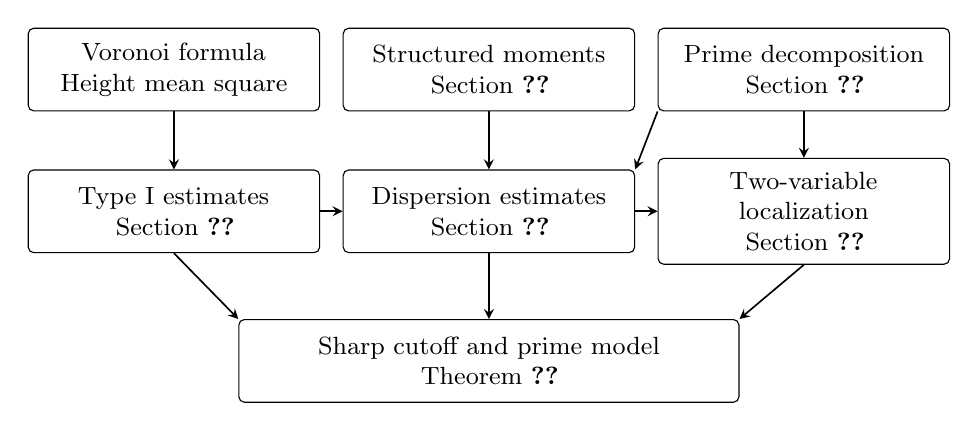
\begin{tikzpicture}[x=1cm,y=1cm,
 box/.style={draw,rounded corners=2pt,align=center,font=\small,
             text width=3.35cm,minimum height=1.05cm,inner sep=5pt},
 arrow/.style={->,>=stealth,semithick}]
\node[box] (level) at (-4,3.4) {Voronoi formula\\Height mean square};
\node[box] (moments) at (0,3.4) {Structured moments\\Section~\ref{sec:dual}};
\node[box] (decomp) at (4,3.4) {Prime decomposition\\Section~\ref{sec:decomposition}};
\node[box] (typei) at (-4,1.6) {Type~I estimates\\Section~\ref{sec:typeI}};
\node[box] (low) at (0,1.6) {Dispersion estimates\\Section~\ref{sec:dispersion}};
\node[box] (high) at (4,1.6) {Two-variable localization\\Section~\ref{sec:perron}};
\node[box,text width=6cm] (end) at (0,-.3) {Sharp cutoff and prime model\\Theorem~\ref{thm:main}};
\draw[arrow] (level)--(typei);
\draw[arrow] (moments)--(low);
\draw[arrow] (typei)--(low);
\draw[arrow] (decomp)--(high);
\draw[arrow] (decomp.south west)--(low.north east);
\draw[arrow] (low)--(high);
\draw[arrow] (typei.south)--(end.north west);
\draw[arrow] (low)--(end);
\draw[arrow] (high.south)--(end.north east);
\end{tikzpicture}

\caption{The proof of the sharp first moment. Solid arrows indicate
uses of proved estimates. The exact prime decomposition supplies the
coefficient classes required by both bilinear branches.}
\label{fig:proof-map}
\end{figure}

Section~\ref{sec:background} states the public arithmetic and analytic
inputs, and Section~\ref{sec:typeI} derives the two Type~I estimates.
The structured moments of Section~\ref{sec:dual} enter the dispersion
estimates of Section~\ref{sec:dispersion}. The exact decomposition is
proved in Section~\ref{sec:decomposition};
Section~\ref{sec:perron} assembles all the estimates, fixes the order of
parameters, and removes the smooth cutoff.
Appendix~\ref{sec:angular} proves the fixed-angular extension, including
the shifted Hecke input, the angular Type~I estimates and the required
twisted sequence condition.

The formal literature inputs are cubic reciprocity and its supplementary
laws; the functional equation, prime ideal theorem, and logarithmic
conductor prime estimates for Hecke characters; Heath-Brown's cubic
large sieve and metaplectic height mean square; and the unconditional
level Voronoi formula and residue of Dunn and Radziwi\l\l.
Their normalizations and uniformity are stated where used. The ordinary
character sieve, the nonsquarefree extensions of the cubic sieve, and
all further cancellation and decomposition arguments are proved here.
In particular, no GRH-dependent cancellation result is an input.

\section{Arithmetic and analytic preliminaries}
\label{sec:background}
\label{sec:preliminaries}

Write $K=\mathbb Q(\omega)$, $\mathcal O=\mathbb Z[\omega]$, and
$\lambda=\sqrt{-3}$, where $\omega=e^{2\pi i/3}$.
An element is \emph{primary} if it is congruent to $1$ modulo $3$.
Every nonzero ideal prime to $3$ has a unique primary generator.
Unless specified otherwise, sums over $a,b,c,d,r,u$ and their divisors
are over these generators. In contrast, Poisson frequencies range over
the full lattice indicated in the formula. We use
\[
 N(z)=|z|^2,\qquad \operatorname{Tr}(z)=z+\overline z,
 \qquad e(x)=\exp(2\pi i x).
\]
The functions $\mu$, $\tau$, and $\varphi$ are the ideal Mobius, divisor,
and Euler functions; thus $\varphi(r)=\#(\mathcal O/(r))^\times$.
The ideal von Mangoldt function is $\Lambda(n)=\log N\pi$ when
$n=\pi^k$ for a prime $\pi$ and $k\ge1$, and is zero otherwise.
We write $\Omega(n)$ for the number of prime factors counted with
multiplicity. The arithmetic function $\Lambda(n)$ is distinguished
by its argument from a completed $L$-function $\Lambda(s,\chi)$.


For a primary prime $\pi$, the cubic residue symbol
$\chi_\pi(v)$ is the element of $\{1,\omega,\omega^2\}$ congruent to
$v^{(N\pi-1)/3}$ modulo $\pi$ when $(v,\pi)=1$, and is zero otherwise.
Extend it multiplicatively in its lower argument. Put
\[
 G(b)=\frac{1}{\sqrt{Nb}}\sum_{v\bmod b}
       \chi_b(v)e\bigl(\operatorname{Tr}(v/b)\bigr),
 \qquad c_* =\frac{(2\pi)^{2/3}}{3\Gamma(2/3)}.
\]
Cubic reciprocity and its supplementary laws, in these conventions,
give $\chi_b(a)=\chi_a(b)$ for primary $a,b$.
The characters $b\mapsto\chi_b(\zeta\lambda^j)$, with $\zeta$ a unit,
have bounded conductor supported above $3$ and trivial infinite
parameter. We use these standard laws in the form recorded in
\cite[Section 2]{DR2024}.

Complete Gauss-sum evaluation and the Chinese remainder theorem give
\begin{equation}
 |G(a)|=\mu^2(a),\qquad
 G(ab)=G(a)G(b)\overline{\chi_b(a)}.
 \label{eq:mult}
\end{equation}
For completeness, the additive character is primitive away from $3$.
At a squarefree modulus the multiplicative character is primitive as
well, so the unnormalized sum has absolute value $\sqrt{Na}$.
At a repeated prime, summation over the final additive lift vanishes,
whereas the multiplicative character is inflated from a smaller modulus.
For coprime $a,b$, the two Chinese-remainder factors give
$\chi_b(a)\chi_a(b)=\overline{\chi_b(a)}$ by reciprocity.
If $(a,b)\ne1$, both sides of the second identity vanish.

For $h\ne0$ that is not a cube in $K$, the character
$b\mapsto\chi_b(h)$ is nonprincipal. Indeed it is the cubic character
of the nontrivial Kummer extension $K(\sqrt[3]{h})/K$.
The splitting criterion at unramified primes, together with the prime
ideal theorem for that extension, proves nontriviality.
Passing to the associated primitive character or adding coprimality
restrictions does not alter this assertion. Since $\mathcal O$ is
integrally closed, an element of $\mathcal O$ that is a cube in $K$
is already a cube in $\mathcal O$.

\subsection{Uniform conventions and classical inputs}

Throughout the proof, $X$ tends to infinity and $L=\log X$.
Lengths refer to norms. All dyads have fixed bounded endpoint ratios;
bounded lengths are allowed. All variables and reciprocal scale
parameters under consideration are bounded by fixed powers of $X$.
A sequence is \emph{divisor-bounded} if its absolute value is at most
$L^C\tau(n)^C$ for some fixed $C$.
Every fixed moment of this majorant on a norm dyad of length $B$ is
$O(BL^{C'})$, with $C'$ fixed. The same assertion holds after collecting
elements having the same rational norm: the number of ideals of norm
$m$, and their divisor multiplicities, are bounded by fixed powers of
the ordinary divisor function. These bounds follow from Euler products
and the usual mean estimates for fixed divisor functions.

The constants in $\ll_\epsilon$ may depend on all fixed support,
smoothness, and coefficient parameters. Each use of $X^\epsilon$ permits
an arbitrarily small positive exponent, chosen after those parameters.
We will explicitly retain logarithmic bounds when a small power loss
would not suffice.

We use Mellin inversion with the convention
\[
 \mathcal MW(s)=\int_0^\infty W(v)v^s\,\frac{dv}{v},\qquad
 W(v)=\frac{1}{2\pi i}\int_{(\sigma)}\mathcal MW(s)v^{-s}\,ds.
\]
Smooth functions in products or ratios of norm variables can consequently
be separated on fixed dyads. At fixed smoothness scale the Mellin
integrands decrease faster than every power of their imaginary
variables. A fixed number of derivatives bounded by powers of $L$
gives corresponding logarithmic costs. Derivative scales smaller than
one will be tracked when they are introduced.

The classical analytic inputs are the functional equation for primitive
Hecke characters, the prime ideal theorem and its Siegel--Walfisz form
over the fixed field $K$, and the ordinary mean-value inequality for
Dirichlet polynomials; see, for general analytic background,
\cite{IwaniecKowalski2004}. For the precise finite-order completion,
see \cite[Section 3.6]{Watkins2011}, and for entireness see
\cite[Section 2C]{ThornerZaman2019}. More precisely, if $\chi$ is primitive with
trivial infinite parameter and conductor norm $D$, then
\[
 \Lambda(s,\chi)
 =\left(\frac{\sqrt{3D}}{2\pi}\right)^s\Gamma(s)L(s,\chi),
 \qquad
 \Lambda(s,\chi)=\varepsilon_\chi\Lambda(1-s,\overline\chi),
 \quad |\varepsilon_\chi|=1.
\]
The field has discriminant $-3$ and one complex place. The complex
gamma factor in \cite{Watkins2011} is
$2(2\pi)^{-s}\Gamma(s)$; dividing the completion by the constant $2$
gives exactly this convention. For a nonprincipal character the
completed function is entire.
For every fixed $A,M>0$, nonprincipal cubic characters with primitive
conductor norm at most $(\log x)^A$ satisfy, uniformly,
\begin{equation}
 \sum_{N\pi\le x}\chi(\pi)\ll_{A,M}x(\log x)^{-M}.
 \label{eq:hecke-sw}
\end{equation}
Here is an explicit route to this uniformity. Apply
\cite[Theorem 1.4]{ThornerZaman2019} to the cyclic cubic extension of
$K$ cut out by $\chi$. Its three characters are
$1,\chi,\overline\chi$, and both nontrivial conductors have norm $D$.
The parameters of that theorem are $n_K=2$, $D_K=3$, and $Q=D$.
Weighting the three Frobenius-class counts by $\chi$ cancels their
principal terms. The possible exceptional character is real; in a
cyclic group of order three it must be trivial, so its term also
cancels. The resulting error is at most a constant times
\[
 \operatorname{Li}(x)\left\{
   \exp\!\left(-\frac{c\log x}{\log(12D)}\right)
       +\exp(-c\sqrt{\log x})\right\}+O(\log(2D)).
\]
For $D\le(\log x)^A$, the theorem's threshold
$x\ge(12D)^{c_2}$ holds eventually, and this error gives
\eqref{eq:hecke-sw} for every fixed $M$. The same theorem for a fixed
extension gives the prime ideal theorem and the nonprincipality test
used above. Standard partial summation gives the smooth and interval
versions of \eqref{eq:hecke-sw}. Any additional omitted Euler factors
will be accounted for through their deleted primes at the point of use.
For coefficients indexed by rational integers we use the classical
mean-value estimate of Montgomery and Vaughan~\cite{MontgomeryVaughan1974},
\begin{equation}
 \int_I\left|\sum_{n\le Z}v_n n^{it}\right|^2dt
 \ll (|I|+Z)\sum_{n\le Z}|v_n|^2,
 \label{eq:ordinary-mean-value}
\end{equation}
where $I$ is any interval. An arbitrary fixed translation of the height
is absorbed into the coefficients.

\subsection{Two large sieves}

\begin{theorem}[Heath-Brown's cubic large sieve]
\label{thm:cls}
Let $A,B\ge1$, and let $(u_b)$ be supported on primary squarefree
elements with $Nb\asymp B$. Then, for every $\epsilon>0$,
\[
 \sum_{Na\asymp A}\mu^2(a)
 \left|\sum_b u_b\chi_a(b)\right|^2
 \ll_\epsilon (AB)^\epsilon
 \bigl(A+B+(AB)^{2/3}\bigr)\sum_b|u_b|^2.
\]
The same assertion holds with upper cutoffs in place of dyads.
\end{theorem}

This is \cite[Theorem 2]{HB2000}. Its squarefree hypotheses apply to
both arguments, and will not be discarded without the following
explicit extensions.

The underlying planar large sieve is the number-field inequality
associated with Huxley~\cite{Huxley1968}; its exact $Z+Q^2$ scale
is also recorded in \cite[Equation (1.2)]{GaoZhao2022}. We give the
primitive-character argument needed here, including the absence of a
small-power conductor loss.

\begin{lemma}[The ordinary character large sieve]
\label{lem:ordinary-sieve}
For distinct primitive ray characters of trivial infinite parameter,
with conductor norm at most $Q$ and with conductor above $3$ dividing
a fixed modulus, and coefficients supported on a norm dyad of length
$Z$, one has
\[
 \sum_\chi\left|\sum_n v_n\chi(n)\right|^2
 \ll (Z+Q^2)\sum_n|v_n|^2.
\]
The implied constant is uniform when a fixed additional modulus above
$3$ is allowed. In particular, the bound applies to the cubic characters
indexed by coprime primary squarefree $p,q$ through
$b\mapsto\chi_b(pq^2)$, whose conductor away from $3$ is $pq$.
There is no $Q^\epsilon$ loss.
\end{lemma}

\begin{proof}
Fixing one of the finitely many classes at the bounded modulus above
$3$ reduces the claim to primitive group characters modulo a primary
$r$, with $Nr\ll Q$.
Let $S(y)=\sum_n v_n e(\operatorname{Tr}(ny))$.
Primitive Gauss-sum expansion and character orthogonality give
\[
 \sum_{\chi\bmod r}^{\mathrm{primitive}}
       \left|\sum_n v_n\chi(n)\right|^2
 \le \frac{\varphi(r)}{Nr}
       \sum_{\substack{h\bmod r\\(h,r)=1}}|S(h/r)|^2
 \le \sum_{\substack{h\bmod r\\(h,r)=1}}|S(h/r)|^2.
\]
Fixed factors arising from the trace-dual lattice are immaterial.
Distinct reduced fractions with denominator norms $O(Q)$ are separated
by $\gg Q^{-1}$ on the dual torus: their difference, after a lattice
translation, has a nonzero integral numerator and denominator of
absolute value $O(Q)$.

The planar additive large sieve for such a separated set has bound
$O(Z+Q^2)$. Here is the usual smoothing argument.
Take a nonnegative Schwartz majorant of the disk containing the support
of $(v_n)$, at scale $\sqrt Z$.
By duality and Poisson summation the resulting Gram matrix has entries
bounded by
\[
 C_N Z\sum_{\ell}(1+\sqrt Z\,|y-y'+\ell|)^{-N}.
\]
Packing a $Q^{-1}$-separated set in successive planar annuli bounds
each row sum by $O(Z+Q^2)$, for a fixed sufficiently large $N$.
The operator norm has the same bound, proving the assertion.
The exponents $1$ and $2$ at the primes dividing $pq$ distinguish the
cubic characters in the last assertion; bounded ramified factors only
introduce a bounded multiplicity.
\end{proof}

\begin{lemma}[Extensions of the cubic large sieve]
\label{lem:cubic-extensions}
The following estimates allow an arbitrarily small $X^\epsilon$ loss.
First, for divisor-bounded coefficients $(v_n)$ of norm length $Z$,
without a squarefree restriction,
\begin{equation}
 \sum_{Na\asymp P}\mu^2(a)
       \left|\sum_n v_n\chi_a(n)\right|^2
 \ll_\epsilon X^\epsilon Z
       \bigl(P+Z+(PZ)^{2/3}\bigr).
 \label{eq:inner-extension}
\end{equation}
Second, for coefficients $(u_b)$ on primary squarefree elements of
norm length $P$,
\begin{equation}
 \sum_{Na\asymp J}\left|\sum_b u_b\chi_b(a)\right|^2
 \ll_\epsilon X^\epsilon
       \bigl(J+(JP)^{2/3}+J^{1/3}P\bigr)\sum_b|u_b|^2.
 \label{eq:outer-extension}
\end{equation}
The latter also holds when $a$ ranges over all nonzero elements of
$\mathcal O$ of norm $\asymp J$. If $J\gg P$, its last term is
absorbed by $(JP)^{2/3}$.
\end{lemma}

\begin{proof}
For the first estimate write uniquely $n=s t^2 c^3$, with $s,t$
coprime and squarefree. Restrict their norms to dyads $S,V,C$, so that
$SV^2C^3\asymp Z$.
For each fixed $t,c$, the factors involving them have modulus at most
one on the outer variable. Apply Theorem~\ref{thm:cls} to the $s$ sum
and then use the triangle inequality in the outer squared-sum norm.
The squared norm of the restricted coefficient sequence is
$O_\epsilon(X^\epsilon S)$.
There are $O(VC)$ choices of $t,c$, and the resulting bound is
\begin{equation}
 X^\epsilon (VC)^2S
       \bigl(P+S+(PS)^{2/3}\bigr).
 \label{eq:inner-extension-dyad}
\end{equation}
Since $(VC)^2S\ll Z$ and $S\ll Z$, summing the logarithmically many
dyads proves \eqref{eq:inner-extension}. We retain
\eqref{eq:inner-extension-dyad} when a restriction makes $S$ shorter.

For the second estimate factor the outer argument in the same way.
Fixing $t,c$ when $S\ge V$, and applying Theorem~\ref{thm:cls} to $s$,
costs
\[
 X^\epsilon VC\bigl(S+P+(SP)^{2/3}\bigr)\sum_b|u_b|^2.
\]
Fixing $s,c$ when $S<V$ gives instead
\[
 X^\epsilon SC\bigl(V+P+(VP)^{2/3}\bigr)\sum_b|u_b|^2,
\]
with character conjugation if necessary.
Using $SV^2C^3\ll J$ and the indicated order of $S,V$, each expression
is bounded by the right side of \eqref{eq:outer-extension}.
The coprimality restriction imposed by $c$ is simply a restriction of
the coefficients for each fixed $c$.
For a full-lattice argument write
$a=\zeta\lambda^i s t^2 c^3$, $i\in\{0,1,2\}$, allowing powers of
$\lambda$ in $c$. The finitely many unit and residual ramified factors
are coefficient twists. The same proof applies.
\end{proof}

\subsection{The unconditional level input}

We use only the unconditional summation formula of Dunn and Radziwill,
not their subsequent estimates that assume GRH. To identify the exact
input, equation numbers in the following statement refer to
\cite[arXiv version 3, Proposition 5.3]{DR2024}.

\begin{theorem}[Level Voronoi formula, the required form]
\label{thm:voronoi-background}
Let $r$ be primary and squarefree, and let $W$ be smooth and compactly
supported in $(0,\infty)$. Put $R=Nr$ and
$A_0=(2\pi)^{5/3}/(3^{7/2}\Gamma(2/3))$.
The completed sum
\[
 \mathcal C_r(V;W)=
 \sum_{\substack{d,u\\(d,r)=1}}|d|G(ur)
             W\left(\frac{N(ud^3)}{V}\right)
\]
has main term
$A_0\mathcal MW(5/6)V^{5/6}\varphi(r)R^{-7/6}$.
Its remaining term is
\[
 \frac{R^{1/2}}{3^{7/2}(2\pi)^2}
 \sum_{\substack{0\ne\nu\in\lambda^{-1}\mathcal O, d\\(d,r)=1}}
 \frac{a_r(\nu)b_r(\nu)}{N\nu\,(Nd)^{5/2}}
 \check W\left(\frac{(2\pi)^4N(d^3\nu)V}{R^2}\right),
\]
where, for sufficiently small $\sigma>0$,
\[
 \check W(v)=\frac{1}{2\pi i}\int_{(-\sigma)}v^z
 \frac{\Gamma(5/6-z)\Gamma(7/6-z)}
      {\Gamma(z-1/6)\Gamma(z+1/6)}\mathcal MW(z)\,dz.
\]
The coefficients depend only on $r$ and $\nu$, independently of $V$
and $W$. They vanish outside representations
\[
 \nu=\lambda^j\zeta h w(h')^3,\quad j\ge-1,\quad
 h,h'\mid r^\infty,\quad (w,r)=1,\quad \mu^2(hw)=1,
\]
where $h,h',w$ are primary and $\zeta$ is a unit.
On this support, they are
\[
 a_r(\nu)=a^\star(\lambda^{-3}\nu),\qquad
 b_r(\nu)=\mu\left(\frac{r}{(\lambda\nu,r)}\right)
          \frac{\varphi(r)}{\varphi\left(r/(\lambda\nu,r)\right)},
\]
where $a^\star$ is the theta coefficient in
\cite[Equation (5.74)]{DR2024}; the second formula is its
Equation (5.68). The index $\lambda^{-3}\nu$ is the one supplied
by its coefficient identity (5.79).
They satisfy
\[
 |a_r(\nu)|\ll 3^{\max(j,0)/3}|h'|,
 \qquad |b_r(\nu)|\le N((\lambda\nu,r)).
\]
In particular, if $V,V^{-1},R\ll X^{C_0}$ for fixed $C_0$, $W$ is
supported in a fixed compact subinterval of $(0,\infty)$, and each
fixed derivative bound is at most a fixed logarithmic power, then
\begin{equation}
 \mathcal C_r(V;W)=
 A_0\mathcal MW(5/6)V^{5/6}\frac{\varphi(r)}{R^{7/6}}
 +O_\epsilon(X^\epsilon R^{1/2}).
 \label{eq:voronoi}
\end{equation}
\end{theorem}

\begin{proof}[Derivation of the stated consequence]
The summation formula and coefficient information are the cited
background theorem, with Equations (5.7), (5.13)--(5.14),
(5.74), and (5.79)--(5.81). In particular, the dual theta coefficient
is read from the proof formula (5.79), where its index is
$\lambda^{-3}\nu$; this avoids the repeated ramified exponent in
the printed (5.67). The theta formulas give
$|a_r(\nu)|\ll3^{\max(j,0)/6}|h'|$, which implies the stated
weaker bound; the finitely many exceptional ramified cases have bounded
factors. Multiplying the original summation formula by $G(r)$ uses
$G(r)\overline{g(r)}=R^{1/2}$, where $g(r)=\sqrt R\,G(r)$.
This proves the displayed normalization of both terms.

We give the absolute convergence argument for \eqref{eq:voronoi}.
On $\operatorname{Re}z=-\sigma$, rapid Mellin decay and Stirling's
formula bound the transform by
\[
 X^{O(\sigma)}L^{O(1)}
              \bigl(N(d^3\nu)\bigr)^{-\sigma}.
\]
For a prime of norm $p$ dividing $r$, the exponents in $h,h'$ are
$e\in\{0,1\}$ and $k\ge0$. Its absolute local sum is bounded by
\[
 \sum_{e=0}^1\sum_{k\ge0}
 p^{1_{e+k>0}}p^{k/2}p^{-(e+3k)(1+\sigma)}
 =1+p^{-\sigma}+O_\sigma(p^{-3/2-3\sigma}).
\]
For every fixed $\eta>0$, the product over $p\mid r$ is
$O_{\sigma,\eta}(R^\eta)$: separate the finitely many small primes,
then bound each remaining factor by $p^\eta$.
The free $w$ sum converges at $1+\sigma$, the ramified sum is dominated
by $\sum_{j\ge0}3^{-j(2/3+\sigma)}$, and the $d$ sum converges at
$5/2+3\sigma$.
Choosing $\sigma$ and $\eta$ sufficiently small in terms of the final
$\epsilon$ proves \eqref{eq:voronoi}.
\end{proof}

\begin{theorem}[The metaplectic mean-square input]
\label{thm:hb-height}
For primary squarefree $r$, the Dirichlet series
\[
 f_r(s)=\sum_u G(ru)(Nu)^{-s},\qquad \operatorname{Re}s>1,
\]
continues meromorphically to $\operatorname{Re}s>1/2$, with at most
a simple pole at $5/6$. It has polynomial growth in closed strips
there, away from its pole. For sufficiently small $\epsilon>0$ and
every $T\ge1$,
\begin{equation}
 \int_{-T}^T|f_r(1/2+\epsilon+it)|^2dt
 \ll_\epsilon (Nr)^{1/2+4\epsilon}T^2.
 \label{eq:hb-mean-square}
\end{equation}
Its residue $\rho_r$ satisfies $|\rho_r|\ll (Nr)^{-1/6}$.
\end{theorem}

The mean-square assertion is \cite[Section 3, Lemma 3]{HB2000}, with
angular index zero; the series there is exactly $f_r$ in this
normalization. We spell out the other analytic properties separately.
Multiplicativity identifies $f_r$ with $G(r)$ times the series in
\cite[Proposition 5.2]{DR2024}. Its completion includes the factor
$\sum_{(d,r)=1}(Nd)^{-(3s-1/2)}$, whose Euler product is nonzero for
$\Rea s>1/2$. Thus division introduces no further pole in this
half-plane. The residue is

\begin{equation}
 \rho_r=A_0\frac{\varphi(r)}{(Nr)^{7/6}}
       \left(\sum_{(d,r)=1}(Nd)^{-2}\right)^{-1}.
 \label{eq:typeI-residue}
\end{equation}
The last sum is at least one, proving the bound without a small power
loss in the level.

For the growth needed in a contour shift, put $R=Nr$. In the notation
of \cite[Section 3, Equation (14)]{HB2000}, write
$Z(q,z)=\zeta_K(3z-2;1_3)\psi(q,z)$, where $1_3$ denotes omission
of the prime above $3$. Equation (19) there bounds this function at
large height by
\[
 |Z(q,\alpha+iy)|\ll_e
 (Nq)^{(3/2+e-\alpha)/2}(1+y^2)^{3/2+e-\alpha},
 \qquad \tfrac12\le\alpha\le\tfrac32.
\]
Only $|y|\ge1$ is used, away from the possible pole. The finite-divisor
identity at the end of that section gives
$f_r(s)=R^s\psi_r(1,s+1/2)$ and, for $\Rea z\ge1+\delta$,
\[
 |\psi_r(1,z)|\ll_\delta R^{-1/2}
       \sum_{d\mid r}(Nd)^{-1/2}|\psi(r/d,z)|.
\]
The inverse zeta factor and the finite Euler factors in this identity
are bounded by absolutely convergent products in that region.
Consequently, for $1/2+\delta\le\sigma\le.9$, $|t|\ge1$, and any
fixed $e,\nu>0$,
\[
 |f_r(\sigma+it)|\ll_{\delta,e,\nu}
 R^{\sigma/2+e/2+\nu}(1+t^2)^{1+e-\sigma}.
\]
Here the divisor sum costs at most $\tau(r)\ll_\nu R^\nu$.

To cover the rest of a strip, set
$S_r(U)=\sum_{Nu\le U}G(ru)$. For $U\ge R^2$,
\cite[Lemma 1]{HB2000}, with its parameter $1/12$, applies because
$R\le(RU)^{1/3}$ and gives
\[
 |S_r(U)|\ll R^{-1/6}U^{5/6}+R^{1/4}U^{3/4}
           \ll R^{1/3}U^{5/6}.
\]
For $1\le U<R^2$ the same final bound follows from the trivial bound
$O(U)$. Abel summation now gives, for $\Rea s>5/6$,
\[
 f_r(s)=s\int_1^\infty S_r(y)y^{-s-1}\,dy,
 \qquad
 |f_r(s)|\ll R^{1/3}\frac{|s|}{\Rea s-5/6}.
\]
This proves polynomial growth on $\Rea s\ge.9$, overlapping the
previous range. Bounded heights away from the pole follow from
meromorphy for each fixed level. These bounds justify the contour
shifts below; their quantitative height estimate is
\eqref{eq:hb-mean-square}.


\section{Type I estimates}
\label{sec:typeI}

The Type I sums have arbitrary coefficients in the level $r$
and a smooth unrestricted sum over $u$. The level formula evaluates
this inner sum after completion by cubes. We remove that completion by
M\"obius inversion: its residue gives the squarefree model, while the
discarded cube divisors are bounded by counting at small levels and by
the cubic large sieve at the remaining levels. At large Mellin heights
we instead estimate the Gauss-sum term directly from the metaplectic
mean square.

\begin{proposition}[Type I comparison]
\label{prop:typeI}
Suppose $RU\asymp X$ and $1\le R\ll X^{.51}$.
Let $(a_r)$ be divisor-bounded and supported on $Nr\asymp R$.
Let $W_r$ have support in a fixed compact subinterval of $(0,\infty)$,
with each fixed derivative bounded by a fixed power of $L$, uniformly
in $r$. Then
\[
 \sum_r a_r\sum_u
 \left(G(ru)-c_*\frac{\mu^2(ru)}{N(ru)^{1/6}}\right)W_r(Nu/U)
 \ll X^{5/6-\eta}
\]
for some fixed $\eta>0$. One may take $\eta=1/100$, with constants
depending on the stated fixed parameters.
\end{proposition}

\begin{proof}
Nonsquarefree $r$ contribute zero to both terms. For squarefree $r$,
invert cube completion by the exact identity
\begin{equation}
 \sum_uG(ru)W_r(Nu/U)
 =\sum_{(c,r)=1}\mu(c)|c|\,
       \mathcal C_r(U/(Nc)^3;W_r).
 \label{eq:inverse-completion}
\end{equation}
Indeed the coefficient at a cube $e^3$ is
$|e|\sum_{c\mid e}\mu(c)$, equal to zero unless $e=1$.
All sums in this identity are finite at the given compact support.
Use \eqref{eq:voronoi} for $Nc\le C_*$, where
\[
 C_*=
 \begin{cases}
 X^{.13},& R\le X^{.40},\\
 X^{.02},& R>X^{.40}.
 \end{cases}
\]
After summing $r$, the total error is
\begin{equation}
 \ll X^\epsilon R^{3/2}C_*^{3/2}\ll X^{.795+\epsilon}.
 \label{eq:short-completion-error}
\end{equation}
The main term, completed to all $c$, is
\begin{equation}
 A_0\mathcal MW_r(5/6)U^{5/6}
 \frac{\varphi(r)}{(Nr)^{7/6}}
 \sum_{(c,r)=1}\frac{\mu(c)}{(Nc)^2}.
 \label{eq:typeI-main}
\end{equation}
Its omitted tail, after summing $r$, is
$O(X^{5/6+\epsilon}C_*^{-1})$.

We compare \eqref{eq:typeI-main} with the model directly.
The coset $1+3\mathcal O$ has Euclidean area density $2/(9\sqrt3)$,
hence radial density $2\pi/(9\sqrt3)$ in the norm variable.
Square-divisor and coprimality inversion show, for a log-smooth
weight $W$, that
\[
 \sum_{(u,r)=1}\mu^2(u)W(Nu/U)
 =\frac{2\pi U}{9\sqrt3}\mathcal MW(1)
       \frac{\varphi(r)}{Nr}
       \sum_{(c,r)=1}\frac{\mu(c)}{(Nc)^2}
       +O_\epsilon(X^\epsilon\sqrt U).
\]
To justify the error, truncate square divisors at $Nc\ll\sqrt U$.
Each relevant sublattice count differs from its area by at most a
constant times one plus its scaled radius. Summing these errors and
the divisors of $r$ costs only $X^\epsilon\sqrt U$; completing the
area term has the same error.
Apply this formula to $v^{-1/6}W_r(v)$ and use
\[
 c_*\frac{2\pi}{9\sqrt3}=A_0.
\]
The model therefore equals \eqref{eq:typeI-main}, with total error
over $r$ bounded by
\begin{equation}
 X^\epsilon R^{5/6}U^{1/3}
 \asymp X^{1/3+\epsilon}R^{1/2}
 \ll X^{.589+\epsilon}.
 \label{eq:typeI-lattice-error}
\end{equation}

It remains to bound the omitted part of \eqref{eq:inverse-completion}.
Combine $c,d$ into $e=cd$, and restrict $Ne$ to a dyad of length
$E\gg C_*$. Its coefficient is divisor-bounded times $E^{1/2}$;
the restriction $(e,r)=1$ may be kept in the outer coefficient.
Trivial counting gives
\begin{equation}
 \ll X^{1+\epsilon}E^{-3/2}.
 \label{eq:typeI-trivial-tail}
\end{equation}
When $R\le X^{.40}$ this is $O(X^{.805+\epsilon})$.

For the other range fix $e$ and put $U_e=U/E^3$.
Using \eqref{eq:mult}, Cauchy in $r$, and
Theorem~\ref{thm:cls}, the bilinear sum in $r,u$ costs
\[
 \ll X^\epsilon\sqrt{RU_e}
       \bigl(R+U_e+(RU_e)^{2/3}\bigr)^{1/2}.
\]
The automatic vanishing restricts both variables to squarefree elements.
Mellin inversion separates the weights; the arbitrary dependence of
$W_r$ on $r$ changes only the outer coefficients and a common
integrable majorant. Summing the absolute $e$ coefficients on the dyad
costs $O(X^\epsilon E^{3/2})$. Thus the tail on that dyad is
\begin{equation}
 \ll X^{1/2+\epsilon}
       \left(R+U/E^3+(X/E^3)^{2/3}\right)^{1/2}.
 \label{eq:typeI-sieve-tail}
\end{equation}
For $X^{.40}<R\ll X^{.51}$ and $E\gg X^{.02}$, its three terms
have exponents at most
\[
 .755,\qquad .77,\qquad
 \frac12+\frac{1-.06}{3}=\frac56-\frac1{50}.
\]
The same last upper exponent bounds the omitted main-term tail in
this range. Equations \eqref{eq:short-completion-error}--
\eqref{eq:typeI-sieve-tail}, with logarithmically many dyads and
sufficiently small epsilon losses, prove the assertion with
$\eta=1/100$.
\end{proof}

\begin{proposition}[Type I at large Mellin heights]
\label{prop:typeIheight}
Suppose $RU\asymp X$, and let $(a_r)$ be divisor-bounded on
$Nr\asymp R$. Suppose the smooth compactly supported weights $W_r$
have fixed support ratios and uniformly bounded derivatives,
independently of $X$. For $T\ge2$ and every fixed $D>0$,
\begin{align}
 &\int_{|t|\asymp T}\sum_{Nr\asymp R}|a_r|
       \left|\sum_uG(ru)(Nu)^{it}W_r(Nu/U)\right|\frac{dt}{T}
 \notag\\
 &\hspace{12mm}\ll_\epsilon
       X^{1/2+\epsilon}R^{3/4}T^{1/2}
       +O_D\bigl(X^{5/6}L^{C}T^{-D}\bigr),
 \label{eq:typeI-height}
\end{align}
where $C$ depends only on the coefficient bounds.
\end{proposition}

\begin{proof}
Again only squarefree $r$ contribute.
For each such $r$, Mellin inversion on a line to the right of one gives
\[
 \sum_uG(ru)(Nu)^{it}W_r(Nu/U)
 =\frac{1}{2\pi i}\int_{(2)}
       \mathcal MW_r(s)U^s f_r(s-it)\,ds.
\]
Shift to $\sigma=1/2+\epsilon'$, with $\epsilon'>0$ small.
Theorem~\ref{thm:hb-height} and rapid Mellin decay justify this shift.
The residue is
\[
 \rho_r U^{5/6+it}\mathcal MW_r(5/6+it)
 \ll_D U^{5/6}R^{-1/6}(1+|t|)^{-D}.
\]
For the new integral use Minkowski and Cauchy in $t$.
For every real $v$, \eqref{eq:hb-mean-square}, applied on a symmetric
interval of radius $O(T+|v|+1)$, gives
\[
 \left(\int_{|t|\asymp T}
       |f_r(\sigma+i(v-t))|^2\frac{dt}{T}\right)^{1/2}
 \ll_{\epsilon'}R^{1/4+2\epsilon'}
              \frac{T+|v|+1}{\sqrt T}.
\]
Since $\mathcal MW_r(\sigma+iv)$ decreases rapidly, uniformly in $r$,
the mean absolute value of the new integral is
\[
 \ll_{\epsilon'} U^{1/2+\epsilon'}R^{1/4+2\epsilon'}\sqrt T.
\]
Finally $\sum_{Nr\asymp R}|a_r|\ll RL^C$.
Summing the last bound and the residues, and taking $\epsilon'$
sufficiently small in terms of $\epsilon$, proves
\eqref{eq:typeI-height}.
\end{proof}

The two applications of Proposition~\ref{prop:typeIheight} are
\[
 R\le X^{.40},\quad T\ll X^{.01},
 \qquad\text{and}\qquad
 R\le X^{1/3-\kappa/2},\quad T\ll X^{1/6+\rho}.
\]
The respective first-term exponents are at most $.805+\epsilon$ and
$5/6-3\kappa/8+\rho/2+\epsilon$.
Both have a fixed power gap when $\rho$ is sufficiently small in terms
of $\kappa$. Above a sufficiently large fixed power of $L$, the pole
term has any prescribed logarithmic saving by choosing $D$ large.

\section{Character moments at the two exceptional configurations}
\label{sec:dual}

This section supplies the power saving needed at the two boundary
configurations of the dispersion argument.  The coefficients have a
restricted but important form: they are convolutions of a bounded number
of prime sequences with independently specified smooth norm weights.
There is no sharp condition coupling the prime factors.

Fix a positive constant $c$, a positive integer $k_0$, and fixed support
and smoothness bounds.  An admissible prime convolution at length $Y$ is
\begin{equation}
 \beta(b)=\mu^2(b)
 \sum_{b=\pi_1\cdots\pi_k}
       \prod_{j=1}^k w_j\bigl(N(\pi_j)/F_j\bigr),
 \qquad 1\le k\le k_0,\qquad \prod_{j=1}^k F_j\asymp Y,
 \label{eq:prime-convolution}
\end{equation}
where the primes are primary, the tuple is ordered, every supported prime
has norm at least $Y^c$, and the $w_j$ have compact support in fixed
subintervals of $(0,\infty)$.  Each fixed derivative is bounded by a fixed
power of $\log Y$, uniformly over the family under consideration.  These
bounds imply fixed divisor bounds for all coefficients below.

For sums $\sum_b\beta(b)\chi_b(pq^2)$, with $p,q$ coprime and
squarefree of norm lengths $P,Q$, the two sieves reach the same bound
at different configurations. At $(P,Q)=(Y,1)$,
Theorem~\ref{thm:cls} gives, up to an arbitrarily small power loss,
the second-moment bound
\[
 Y\bigl(Y+Y+Y^{4/3}\bigr)\ll Y^{7/3}.
\]
At $P=Q=Y^{1/3}$ the conductor norm is $O(PQ)=O(Y^{2/3})$, so
Lemma~\ref{lem:ordinary-sieve} gives $Y(Y+Y^{4/3})\ll Y^{7/3}$,
again up to an arbitrarily small power loss. These are the two
configurations left by the dispersion argument below. The convolution
structure permits a fixed power saving in neighborhoods of both.

\begin{proposition}[The exceptional character moments]
\label{prop:dual}
There are constants $\delta,\eta>0$, depending only on the fixed data in
\eqref{eq:prime-convolution}, with the following property.  Let
$v,e\in\mathcal O\setminus\{0\}$ satisfy
$N(v),N(e)\le Y^\delta$, and let $1+|u|\le Y^{0.36}$.  Put
\[
 A(p,q)=\sum_{(b,e)=1}\beta(b)N(b)^{iu}\chi_b(vpq^2).
\]
If $p,q$ run through coprime primary squarefree elements of respective
norm lengths $P,Q\ge1$, and either
\[
 \left|\frac{\log P}{\log Y}-1\right|\le\delta,
 \qquad 0\le\frac{\log Q}{\log Y}\le\delta,
\]
or
\[
 \left|\frac{\log P}{\log Y}-\frac13\right|\le\delta,
 \qquad
 \left|\frac{\log Q}{\log Y}-\frac13\right|\le\delta,
\]
then
\begin{equation}
 \sum_{p,q}|A(p,q)|^2\ll Y^{7/3-\eta}.
 \label{eq:exceptional-moment}
\end{equation}
The implied constant is uniform for the specified support and
smoothness bounds.
\end{proposition}

The short convolution identity used in the proof replaces each prime
sum by products of truncated Mobius sums and full smooth sums.
A factor of essentially full length is shortened by the functional
equation. Otherwise, moments of products with factors repeated or
omitted rule out the second configuration and force a precise relation
between factor length and value in the first. There the off-diagonal
Gram estimate supplies the final contradiction. We first prove the two
analytic estimates needed for these alternatives. Throughout, the
unrestricted-inner form of Lemma~\ref{lem:cubic-extensions} permits
divisor-bounded coefficients that need not be squarefree.

In the next lemma a full sum means the complete ideal sum of the
primitive Hecke $L$-function. A restriction excluding primes above $3$,
or other missing Euler factors, is first removed by inclusion--exclusion;
this is carried out explicitly in the dominant-full-sum argument below.

\begin{lemma}[A full smooth sum and its dual]
\label{lem:smooth-character-duality}
Let $\chi$ be a primitive nonprincipal Hecke character of trivial
infinite parameter and conductor norm $D$. Let $W$ be smooth and supported in a
fixed compact subinterval of $(0,\infty)$, with each fixed derivative
bounded by a fixed power of $\log Y$. The full sum
$\sum_n W(N(n)/Z)\chi(n)N(n)^{it}$ admits a decomposition into dual
norm dyads
\[
 J\ll Y^\epsilon D(1+|t|)^2/Z
\]
with amplitude $O(Y^\epsilon\sqrt{Z/J})$.  The coefficients in a dual
dyad are divisor-bounded, and its character is $\overline\chi$.
All additional norm shifts can be integrated against a common
conductor-independent $L^1$ majorant of mass $O(Y^\epsilon)$.
The omitted tail is smaller than any prescribed negative power of $Y$,
provided the lengths and heights are bounded by fixed powers of $Y$.
\end{lemma}

\begin{proof}
Write
$\widetilde W(s)=\int_0^\infty W(x)x^s\,dx/x$.  Fixed logarithmic
factors in the coefficients can be included in $W$.
Mellin inversion expresses the sum as
\[
 \frac1{2\pi i}\int \widetilde W(s)Z^s L(s-it,\chi)\,ds.
\]
The character is nonprincipal, so shifting the contour to the left
crosses no pole of the $L$-function.  Up to fixed field constants, its
functional equation is
\[
 L(s,\chi)=\epsilon(\chi)D^{1/2-s}
       \frac{\Gamma(1-s)}{\Gamma(s)}L(1-s,\overline\chi),
 \qquad |\epsilon(\chi)|=1.
\]
On a sufficiently far-left line the dual Dirichlet series is absolutely
convergent.  Partition it into smooth norm dyads there.  Stirling's
formula and the rapid decay of $\widetilde W$ show that dyads beyond
$Y^\epsilon D(1+|t|)^2/Z$ have an arbitrarily small total tail.
This truncation is performed before moving the retained, finite dyads
back to the line $\Re s=1/2$.

On that line, with $s=1/2+i\tau$, the integrand for a retained dyad is
$\sqrt Z\,\widetilde W(1/2+i\tau)$ times
\begin{equation}
 \epsilon(\chi)D^{i(t-\tau)}Z^{i\tau}
 \frac{\Gamma(1/2-i(\tau-t))}
      {\Gamma(1/2+i(\tau-t))}
 \sum_{N(n)\asymp J}
       \overline\chi(n)N(n)^{-1/2+i(\tau-t)}w_J(N(n)/J).
 \label{eq:symmetry-line-character}
\end{equation}
The multiplier preceding the polynomial has absolute value one.
In particular, its conductor and root-number dependence is a scalar
for each character, not a change in the coefficients of the polynomial.
The gamma poles lie to the right of this move.  Extracting $J^{-1/2}$
from the polynomial proves the amplitude assertion.  Rapid Mellin
decay gives a common $L^1$ majorant in $\tau$, including any fixed
logarithmic derivative costs.  Minkowski's inequality in a square-sum
norm over characters therefore applies with the same shifts for every
character.  A common cutoff based on the largest conductor in the
average is permissible by the earlier far-left tail estimate.
\end{proof}

\begin{lemma}[An off-diagonal Gram estimate]
\label{lem:character-gram}
Let $p$ be primary squarefree with $N(p)\asymp P$, and let $W$ be a
fixed smooth radial norm weight of compact support in $(0,\infty)$.
For primary squarefree $p'$ of the same norm length put
\[
 T_{p,p'}=\sum_{n\equiv1\, (3)}
     W(N(n)/Z)\chi_p(n)\overline{\chi_{p'}(n)}.
\]
For $Z\ge1$ and every $\epsilon>0$,
\begin{equation}
 \sum_{p'\ne p}|T_{p,p'}|^2
 \ll_\epsilon (PZ)^\epsilon
      Z\left(P+(P^3/Z)^{2/3}\right).
 \label{eq:near-orthogonality}
\end{equation}
The same bound holds with a subset of the available $p'$.
\end{lemma}

\begin{proof}
Fix $k=(p,p')$, put $K=N(k)$, and write $p=ka$, $p'=kb$.
The remaining moduli $a,b$ are coprime and squarefree.  The common
factor contributes the restriction $(n,k)=1$.  Remove this restriction
by summing over $m\mid k$ with coefficient $\mu(m)$, and put $M=N(m)$.
After $n=mx$, the character is
$\psi(x)=\chi_a(x)\overline{\chi_b(x)}$, apart from a scalar of
absolute value one.  It is primitive modulo $ab$ and nonprincipal:
the only principal case would be $a=b=1$, contrary to $p'\ne p$.

Apply Poisson summation on $x\equiv1\pmod3$ modulo $3ab$.
The zero frequency vanishes.  Primitive Gauss evaluation gives
amplitude
\[
 \asymp\frac{Z}{M\sqrt{N(ab)}}\asymp\frac{ZK}{MP},
\]
and natural dual norm length
\[
 J_0\asymp\frac{N(ab)M}{Z}
       \asymp\frac{P^2M}{K^2Z}.
\]
For clarity about the subsequent sieve application, the complete
Gauss factor and CRT unit factors are independent of the frequency.
They are scalars for each $b$.  The frequency character is
$\overline{\chi_a(h)}\chi_b(h)$, and the primary residue condition
adds only a fixed bounded-modulus phase.  The Fourier transform is
radial, so its remaining dependence on $b$ is through its norm.

More explicitly, set $c=ab$ and
$g(\psi)=\sum_{x\bmod c}\psi(x)e(\operatorname{Tr}(x/c))$.
Writing the primary residue classes as $x=c+3s$ gives the complete
finite Fourier coefficient
\[
 e\left(\operatorname{Tr}\frac{h}{3\lambda}\right)
       \psi(3\lambda)\overline{\psi(h)}g(\psi)
 =e\left(\operatorname{Tr}\frac{h}{3\lambda}\right)
       \overline{\psi(h)}g(\psi),
\]
because $3\lambda=(-\lambda)^3$. This also displays directly why
no varying-modulus factor remains inside the frequency coefficients.

On a frequency dyad $N(h)\asymp J$, Mellin separation in the compact
scaled variables $N(h)/J$ and $N(b)/(P/K)$ gives coefficients
independent of $b$, integrated against a rapidly decreasing common
majorant.  For every fixed $A>0$ its mass is
$O_A((1+J/J_0)^{-A})$; derivatives have the same property after
adjusting $A$.  Units and exact powers of the ramified prime in $h$
can be separated first.  Their character values are again rowwise
scalars, and the number of cases costs an arbitrarily small power.
The extension with unrestricted inner coefficients in
Lemma~\ref{lem:cubic-extensions} now bounds this dyad, after squaring
and summing over $b$, by
\[
 (PZ)^\epsilon
 \left(\frac{ZK}{MP}\right)^2
 J\left(\frac PK+J+(PJ/K)^{2/3}\right)
 (1+J/J_0)^{-A}.
\]
The restrictions on $b$ may be dropped in this upper bound.

Sum the frequency dyads, retaining the rapid decay also when
$J_0<1$.  The three powers of $J$ are $1,2,5/3$; for $A$ sufficiently
large their dyadic sums are bounded by the corresponding powers of
$J_0$.  Substitution gives the three terms
\[
 \frac{ZP}{MK},\qquad \frac{P^2}{K^2},\qquad
 \frac{P^2Z^{1/3}}{K^2M^{1/3}}.
\]
Since $Z,K,M\ge1$, their sum is
$O(ZP+P^2Z^{1/3})$.  There are only a divisor-bounded number of
choices $k\mid p$ and $m\mid k$.  Cauchy's inequality over those
choices, with a rechoice of $\epsilon$, proves
\eqref{eq:near-orthogonality}.
\end{proof}

\begin{proof}[Proof of Proposition~\ref{prop:dual}]
We use a limiting-exponent contradiction, and give the uniformity
argument explicitly at the end.  Thus suppose that along a sequence
$Y\to\infty$ the extra twist and exclusion norms are $Y^{o(1)}$,
the pair of length exponents tends to $(1,0)$ or $(1/3,1/3)$, and
the moment is at least $Y^{7/3-o(1)}$.  Throughout this proof, a
subpower loss means a bound with an arbitrarily small fixed positive
power loss; it is never used as a logarithmic saving.

\smallskip
\noindent\emph{Prime powers and repeated factors.}
First remove the squarefree restriction in
\eqref{eq:prime-convolution}, and replace each prime weight by its
smooth $\Lambda/\log N$ counterpart.  The resulting discrepancy has
divisor-bounded coefficients on a set of size $O(Y^{1-\theta})$ for
some fixed $\theta>0$.  Indeed every discrepancy contains either a
repeated prime of norm at least $Y^c$, or a prime power of exponent
at least two and norm at least $Y^c$.  In either case its squareful
part has positive-power norm.  In the canonical factorization
$b=st^2d^3$, with $s,t$ coprime squarefree, this also implies
$N(s)\le Y^{1-\theta'}$ for some fixed $\theta'>0$.
To include prime powers with a small base, if $\pi^j$ has $j\ge2$
and $N(\pi^j)\ge Y^c$, then
$N(b/s)\ge N(\pi^j)^{1/2}\ge Y^{c/2}$.
Also $b$ is divisible by the square of
$\pi^{\lfloor j/2\rfloor}$, whose norm is at least $Y^{c/4}$.
Summing $O(Y/N(d)^2)$ over square divisors with $N(d)\ge Y^{c/4}$
gives support size $O(Y^{1-c/4})$. Repeated large primes satisfy the
same bounds, with room to spare.

In the first configuration fix $q$, at a subpower cost. In the
factorization $b=st^2d^3$, let $S,V,C$ be the dyadic norms of $s,t,d$.
Then $SV^2C^3\asymp Y$ gives $(VC)^2S\ll Y$, while
$S\ll Y^{1-\theta'}$. Substituting these
two bounds in \eqref{eq:inner-extension-dyad}, and summing the dyads,
bounds the discrepancy moment by
\[
 Y^{1+o(1)}
 \left(Y+Y^{1-\theta'}+Y^{(4-2\theta')/3}\right),
\]
which saves a power.  In the second configuration, square the
discrepancy polynomial.  Its support has size at most
$Y^{2-2\theta}$ and its coefficients remain divisor-bounded.
The ordinary character sieve, at polynomial length $Y^2$ and
conductor norm at most $Y^{2/3+o(1)}$, therefore bounds its fourth
moment by $Y^{4-2\theta+o(1)}$.  Cauchy's inequality over
$Y^{2/3+o(1)}$ characters gives a second moment at most
$Y^{7/3-\theta+o(1)}$.  The fixed extra character and exclusions are
part of the coefficients in these applications.  Hence both
discrepancies can be discarded.

\smallskip
\noindent\emph{A short convolution identity.}
Here $*$ denotes Dirichlet convolution on ideals and $1$ is the
constant-one arithmetic function. For a prime-polynomial dyad with
upper endpoint $F'$, let
$m=\mu\,1_{N\le\sqrt{F'}}$ and let $\mathbf1_*$ denote the
convolution identity.  The function $\mathbf1_*-m*1$ vanishes up to
norm $\sqrt{F'}$, so its convolution square vanishes up to norm
$F'$.  Convolving with $\Lambda$ and using $1*\Lambda=\log N$
gives, on the dyad,
\begin{equation}
 \Lambda=(2m-m*m*1)*\log N.
 \label{eq:short-mobius-identity}
\end{equation}
Apply this identity to every factor, insert smooth norm dyads, and
separate the original product weights by Mellin inversion.  The
number of pieces and the $L^1$ costs are subpower.  Rapid Mellin
decay permits truncation of additional shifts at $Y^\epsilon$;
the tails are negligible by trivial bounds.  Minkowski's inequality
permits fixing the same shifts across each character average.

It follows that some product of a bounded number of divisor-bounded
character polynomials still has second moment
$Y^{7/3-o(1)}$.  Pass to a subsequence on which their length
exponents tend to
\[
 a_i\ge0,\qquad \sum_i a_i=1.
\]
The common norm twists and fixed character factors can be distributed
multiplicatively over these polynomials.  Every truncated Mobius
factor has length at most $Y^{1/2+o(1)}$.  Thus, if an $a_i$ is one,
that factor is a full smooth sum, with logarithmic factors allowed,
and with twist height at most $Y^{0.37}$.

\smallskip
\noindent\emph{A dominant full sum.}
Suppose that $a_i=1$.  All other factors have subpower trivial size.
The character in the full sum is nonprincipal.  Its conductor away
from the fixed ramified part agrees with $pq$ except at primes
dividing the subpower extra twist or exclusion number.  Partition
according to the part of $pq$ at those primes and their local
character values, and remove missing Euler factors by
inclusion-exclusion.  There are subpowerly many possibilities.
For each one the rescaled full-sum length is still $Y^{1+o(1)}$;
outside the fixed small parts, the variable character is the original
cubic character or its conjugate.  Exact powers of the ramified
prime can likewise be separated on the dual side.
In detail, let $S$ be the primes dividing $3ve$, fix the $S$ parts
of $p,q$, and fix the resulting primitive local character $\psi_S$.
There are $Y^{o(1)}$ choices, since the product of the relevant small
prime norms is subpower. The remaining primitive character is
$\psi_S\chi_{p_0}\chi_{q_0}^2$, with $(p_0q_0,S)=1$.
Inclusion-exclusion for missing Euler factors rescales by a fixed
subpower divisor before the functional equation is applied.
On the dual side $\overline{\psi_S}$ is a fixed coefficient twist;
its root number and conductor phase are rowwise scalars as in
\eqref{eq:symmetry-line-character}. The surviving $p_0$, or $p_0q_0$,
has positive-power norm, so this primitive character is nonprincipal.

Apply Lemma~\ref{lem:smooth-character-duality}.  In the second
configuration the conductor is at most $Y^{2/3+o(1)}$, so the trivial
dual estimate is
\[
 |\text{full sum}|\ll Y^{1/3+0.37+o(1)}.
\]
Summing squares over the available characters has exponent at most
$2/3+2(1/3+0.37)<7/3$.  In the first configuration fix $q$ and the
small parts.  The variable squarefree conductor has length
$Y^{1+o(1)}$, and the dual polynomial has length
$J\le Y^{0.74+o(1)}$, allowing an arbitrarily small fixed power
loss.  The cubic sieve with unrestricted inner coefficients gives
\[
 Y^{1+o(1)}\left(Y+J+(YJ)^{2/3}\right)
 \le Y^{2.16+o(1)}.
\]
Both estimates contradict the unsaved moment.  The averaging here is
legitimate precisely because the conductor-dependent factors in
\eqref{eq:symmetry-line-character} are outside each polynomial.

\smallskip
\noindent\emph{Moments of different lengths.}
We may now assume that every $a_i<1$.  Pigeonhole the absolute values
of the individual polynomials.  Values smaller than a sufficiently
large fixed negative power of $Y$ can be discarded using the trivial
bounds for the other factors and the number of characters.  After a
further subsequence, there is a set of $R$ rows on which their
absolute values are $Y^{v_i+o(1)}$, where $v_i\le a_i$, and
\begin{equation}
 r:=\lim\frac{\log R}{\log Y}\ge\frac73-2v,
 \qquad v=\sum_i v_i.
 \label{eq:dual-large-values}
\end{equation}

In the second configuration, cardinality gives $r\le2/3$.
The ordinary sieve applied to the square of the full product gives
$r+4v\le4$.  Together with \eqref{eq:dual-large-values}, these imply
$v=5/6$ and $r=2/3$.  There is therefore an index with
$0<a_i<1$ and $v_i\ge5a_i/6$.  Multiply the full product by this
additional factor, and put $z=1+a_i\in(1,2)$.  Its value on the
chosen rows has exponent at least $5z/6$.  The ordinary sieve yields
\[
 r\le \max(4/3,z)+z-5z/3
      =\max(4/3,z)-2z/3<2/3,
\]
a contradiction.

In the first configuration fix $q$ without changing the limiting
inequality \eqref{eq:dual-large-values}.  The rows are now distinct
squarefree $p$ of length $Y^{1+o(1)}$.  Put
$d_i=v_i-5a_i/6$.  For any fixed nonnegative integer multiplicities
$k_i$ such that $z=\sum_i k_i a_i\in[1/2,2]$, the corresponding
product is a divisor-bounded polynomial of length $Y^{z+o(1)}$.
The unrestricted-inner cubic sieve gives
\begin{equation}
 r\le \frac23-2\sum_i k_i d_i.
 \label{eq:dual-multiplicity}
\end{equation}
Here we used
\[
 z+\max\{1,z,2(1+z)/3\}=\frac23+\frac{5z}{3}
 \qquad (1/2\le z\le2).
\]
The all-ones multiplicity vector makes the right side of
\eqref{eq:dual-multiplicity} equal to the lower bound in
\eqref{eq:dual-large-values}.  Increasing any one multiplicity
therefore proves $d_i\le0$.  Decreasing it proves $d_i\ge0$ whenever
$a_i\le1/2$.  Thus all short factors have $d_i=0$, including factors
with $a_i=0$.

There is at most one index with $a_i>1/2$.  If there is one, remove
it and use copies of a positive short factor to obtain a length
exponent in $[1/2,2]$.  Such a short factor exists because no $a_i$
is one.  Equation~\eqref{eq:dual-multiplicity} then gives
$r\le2/3$, forcing the remaining $d_i\ge0$ as well.  Consequently
all $d_i=0$ and $r=2/3$.

Choose a positive short exponent $a\le1/2$.  Some fixed integer
multiple of $a$ lies strictly between $4/3$ and $2$, since the
width of that interval exceeds $a$.  Taking the corresponding
copies produces a divisor-bounded polynomial of length
$Z=Y^{z+o(1)}$, with $4/3<z<2$, whose values are
$Y^{5z/6+o(1)}$ on at least $Y^{2/3-o(1)}$ distinct squarefree rows.
The integer multiplicity is fixed after passing to the subsequence;
it does not grow with $Y$, even when the limiting $a$ is small.

\smallskip
\noindent\emph{Near orthogonality.}
Choose a nonnegative smooth radial weight equal to at least one on
the support of this last polynomial.  Weighted Cauchy and the
row-sum bound for its Gram matrix give the classical
Bombieri--Hal\'asz--Montgomery inequality; see
\cite[Theorem~1, equation~(1)]{HarcosBHM} for this Hilbert-space step.
In the present notation it gives
\[
 RY^{5z/3+o(1)}
 \le ZY^{o(1)}
       \left(O(Z)+\max_p\sum_{p'\ne p}|T_{p,p'}|\right).
\]
The support ratio is fixed, since the number of copied factors is
fixed.  Lemma~\ref{lem:character-gram}, with
$P=Y^{1+o(1)}$, bounds each squared off-diagonal row sum by
\[
 Y^{o(1)}Z\left(Y+(Y^3/Z)^{2/3}\right).
\]
After dividing the Gram inequality by $ZR$, the left side has
exponent $2z/3$.  The diagonal has exponent at most $z-2/3$, and
Cauchy's inequality bounds the off-diagonal average by exponent
\[
 \frac{z+\max(1,2-2z/3)-2/3}{2}.
\]
Both are strictly less than $2z/3$: the diagonal gap is $(2-z)/3$;
the other gap is $(3z-4)/6$ for $z\le3/2$, and $(z-1)/6$ for
$z\ge3/2$.  These positive gaps absorb every arbitrarily small
fixed power loss and give the final contradiction.

\smallskip
\noindent\emph{Uniform neighborhoods.}
If the proposition failed for every positive neighborhood size and
power saving, choose successively shrinking neighborhood sizes and
savings, and then arbitrarily large counterexamples.  A diagonal
sequence would have extra twist and exclusion norms $Y^{o(1)}$,
length exponents tending to one of the specified pairs, and moment
at least $Y^{7/3-o(1)}$.  There are only boundedly many factors, and
their length exponents lie in a compact simplex.  The preceding
pigeonholing also confines all relevant value exponents to a fixed
compact interval.  The proof therefore applies to a subsequence of
these counterexamples.  Every selected multiplicity and every
small power loss is fixed before taking the limit.  The resulting
contradiction proves the existence of fixed $\delta,\eta>0$ and
the asserted uniform bound.
\end{proof}

\section{Corrected dispersion}
\label{sec:dispersion}

The correction in this section is the cubic-frequency term in Poisson
summation. This is the dispersion mechanism used by Dunn and
Radziwi\l\l~\cite[Section 9, Propositions 9.1--9.2]{DR2024}.
Their squarefree majorant and cube-frequency correction guide the
argument. The noncube estimates and the Type~I mixed-term comparison
are proved here with the unconditional inputs of the preceding sections.
We keep track of the coefficient restrictions
and the frequency ranges needed here; the two exceptional ranges will be
handled by Proposition~\ref{prop:dual}.

Throughout the section, put
\begin{equation}
 AB\asymp X,\qquad X^{0.32}\le B\ll X^{1/2},\qquad
 H=\frac{B^2}{A},\qquad \mathcal Q=ABH^{1/3},\qquad L=\log X.
 \label{eq:dispersion-scales}
\end{equation}
All sums over letters denoting ideals use primary generators prime to
$3$, unless a full lattice is expressly specified. Let $\beta_b$ be
divisor-bounded, supported on squarefree $b$ with $Nb\asymp B$. When
$B>X^{0.40}$, suppose in addition that $\beta$ is a squarefree-restricted
convolution of a fixed number of prime sequences of the kind in
Proposition~\ref{prop:dual}, each prime having norm at least $X^c$ for
some fixed $c>0$. The weights on the individual prime dyads are smooth;
there is no additional cutoff coupling their products. Set
\begin{equation}
 \begin{aligned}
 \beta_b(u)&=\beta_b(Nb)^{iu},&
 S(u)&=\sum_b\beta_b(u)(Nb)^{-1/6},\\
 F_u(a)&=\sum_b\beta_b(u)G(b)\overline{\chi_b(a)}.
 \end{aligned}
 \label{eq:dispersion-polynomials}
\end{equation}
Let $W$ be a nonnegative radial smooth function, bounded in absolute
value and supported in a fixed annulus in $\mathbb C$, and write
$W_A(a)=W(a/\sqrt A)$.

The low-height assertion uses the following property of $\beta$:
\begin{quote}
\emph{(SW)} For every fixed conductor log-power and every fixed
norm-height log-power, the sum of $\beta_b$ against a nonprincipal cubic
Hecke character of the indicated conductor, with a norm twist of the
indicated height, is $O_D(BL^{-D})$ for every $D>0$. The same assertion
holds after imposing coprimality to any specified element of norm
$X^{O(1)}$.
\end{quote}
The implied constants are uniform in these characters, twists, and
exclusions. The fixed powers in the divisor bounds are chosen before any
roughness parameter below.

\begin{proposition}[Dispersion estimates]
\label{prop:dispersion}
Under the preceding hypotheses the following assertions hold.
\begin{enumerate}
\item If $H\gg1$ and $|u|\le X^{0.17}$, and the derivatives of $W$ are
bounded independently of $X$, then
\[
 \sum_a W_A(a)|F_u(a)|^2\ll \mathcal Q L^{O(1)}.
\]
\item Suppose $|u|\le L^{O(1)}$, $H\gg1$, and $\beta$ has property
\emph{(SW)} and is supported on elements all of whose prime factors have
norm greater than $L^{C_r}$. For every fixed $K>0$, if $C_r,C_g$ are
sufficiently large, then for $H\ge L^{C_g}$,
\begin{equation}
 \sum_a\mu^2(a)W_A(a)
 \left|F_u(a)-c_*\overline{G(a)}(Na)^{-1/6}S(u)\right|^2
 \ll \mathcal Q L^{-K}.
 \label{eq:dispersion-corrected}
\end{equation}
For $1\ll H<L^{C_g}$ one has the uncorrected estimate
\begin{equation}
 \sum_a W_A(a)|F_u(a)|^2
 \ll A\sum_b|\beta_b|^2+
 \mathcal Q\left\{\left(B^{-1}\sum_b|\beta_b|\right)^2+L^{-K}\right\}.
 \label{eq:dispersion-short}
\end{equation}
Here $1\ll H$ means only that $H$ is bounded below by a positive
constant. In these low-height assertions the derivatives of $W$ are
bounded independently of $X$.
\item Suppose $u=\pm t+u_0$, $T\le |t|\le2T$,
$2T+|u_0|\le X^{0.17}$, and
$|\partial^jW|\ll_j L^{Cj}$ for fixed $C$. For every fixed $K>0$, if
$T\ge L^{C_t}$ with $C_t$ sufficiently large, then
\begin{equation}
 \int_{T\le|t|\le2T}\sum_a W_A(a)|F_{\pm t+u_0}(a)|^2\frac{dt}{T}
 \le \int_{T\le|t|\le2T}\mathcal D_W\frac{dt}{T}
       +O(\mathcal Q L^{-K}),
 \label{eq:dispersion-height}
\end{equation}
where the exact diagonal is
\[
 \mathcal D_W=\sum_b|\beta_b|^2
                  \sum_{(a,b)=1}W_A(a).
\]
No lower bound on $H$ is required here. When $B\le X^{0.40}$ the
restriction on $u_0$ can be omitted.

There is also an absolute sufficiently small $\gamma>0$ such that, when
$B\le X^{0.40}$, $T\gg X^{0.01}$, and
$|\partial^jW|\ll_j X^{j\gamma}$, the corresponding estimate is
\begin{equation}
 \int_{T\le|t|\le2T}\sum_a W_A(a)|F_{\pm t+u_0}(a)|^2\frac{dt}{T}
 \le \int_{T\le|t|\le2T}\mathcal D_W\frac{dt}{T}
       +O(\mathcal Q X^{-10\gamma}).
 \label{eq:dispersion-power}
\end{equation}
This $\gamma$ is independent of the fixed powers in the divisor bounds.
In the last two estimates, a radial support of width $O(J^{-1})$ gives
\[
 \mathcal D_W\ll \frac AJ\sum_b|\beta_b|^2
\]
for $J\le L^{O(1)}$, or $J\le X^\gamma$, respectively. In particular,
when $B\le X^{0.40}$, the coefficients may be restricted sharply to any
norm cell without changing these assertions.
\end{enumerate}
\end{proposition}

\begin{proof}
Opening the second moment isolates its diagonal; Poisson summation
expresses the off-diagonal part in frequencies.
For \eqref{eq:dispersion-corrected}, the cube
contributions identified below produce the model square, while the
noncube contribution is small. The Type~I comparison supplies the
matching mixed term, giving cancellation in the corrected square.
For the height averages, averaging makes the cube contributions small
as well, leaving the exact diagonal needed for norm localization.
We establish the shared frequency bounds before evaluating the cube
main term and completing that cancellation.

All arbitrarily small power losses below come from Heath-Brown's cubic large
sieve~\cite{HB2000}, in the forms of
Theorem~\ref{thm:cls} and Lemma~\ref{lem:cubic-extensions}; they will be
chosen smaller than the fixed power gaps. For logarithmic savings at
small conductors we instead use Lemma~\ref{lem:ordinary-sieve}, with no
such loss.

\paragraph{Squarefree majorization.}
Only for \eqref{eq:dispersion-corrected}, majorize the squarefree weight
in the positive $|F_u(a)|^2$ term by
\begin{equation}
 \mu^2(a)\le
 \left(\sum_{\substack{c^2\mid a\\Nc\le L^{D_0}}}\mu(c)\right)^2
 =\sum_{d^2\mid a}\lambda_d.
 \label{eq:dispersion-sieve}
\end{equation}
The inequality is equality on squarefree $a$. Expanding the square shows
that $d$ is squarefree, $Nd\le L^{2D_0}$,
$|\lambda_d|\le\tau(d)^2$, and $\lambda_d=\mu(d)$ for $Nd\le L^{D_0}$.
For the uncorrected estimates take only $d=1$, with coefficient one.
The mixed and model terms of the corrected square will retain their
true squarefree weights.

The diagonal is $\mathcal D_W$ when $d=1$. In the sieved case it is
$O(AB L^{O(1)})$: for example, sum
$|\lambda_d|A/(Nd)^2$ and use the coefficient second moment. This is
$O(\mathcal Q L^{-K})$ once $H\ge L^{C_g}$ with $C_g$ large enough.

\paragraph{Poisson summation.}
For an off-diagonal pair write
\[
 f=(b_1,b_2),\qquad b_i=fp_i,\qquad F=Nf,
\]
so that $p_1,p_2$ are coprime, squarefree, prime to $f$, and have norm
$\asymp B/F$. The summand vanishes unless $(b_1b_2,d)=1$. Remove the
remaining restriction $(a,f)=1$ by Mobius inversion, and write
\[
 a=d^2mx,\qquad m\mid f,\qquad M=Nm,\qquad D_d=Nd.
\]
Use normalized plane measure and Fourier transform
\[
 d\mathfrak m(z)=\frac2{\sqrt3}\,d\Re z\,d\Im z,
 \qquad
 \widehat W(y)=\int_{\mathbb C}W(z)e(-\operatorname{Tr}(zy))
                                      \,d\mathfrak m(z).
\]
Poisson summation gives, for this pair and these $d,m$, the following
expression, to be multiplied by $\lambda_d\mu(m)$:
\begin{equation}
\begin{split}
 &\frac{A}{9D_d^2M}
  \frac{\beta_{fp_1}(u)\overline{\beta_{fp_2}(u)}}{|p_1p_2|}
  \sum_{\substack{h\in\mathcal O\\h\ne0}}
  e\left(\operatorname{Tr}\frac{h}{3\lambda}\right)
  \widehat W\left(
    \frac{h\sqrt A}{3\lambda D_d\sqrt M\,p_1p_2}\right)\\
 &\hspace{35mm}\cdot
  \chi_{p_1}\bigl(dh(fm)^{-1}\bigr)
  \overline{\chi_{p_2}\bigl(dh(fm)^{-1}\bigr)}.
\end{split}
\label{eq:poisson}
\end{equation}
The inverses here and below are residue-class notation.

Here are the arithmetic details of this identity. The trace-dual lattice
of $\mathcal O$ is $\lambda^{-1}\mathcal O$. Thus the modulus
$3p_1p_2$ has index $9N(p_1p_2)$, and the dilation contributes
$A/(D_d^2M)$. Since $d,m$ are primary, $x$ must be primary. Put
$q=p_1p_2$ and represent this coset by $x=q+3s$, $s$ modulo $q$.
Its additive factor is
\[
 e\left(\operatorname{Tr}\frac{h}{3\lambda}\right)
 e\left(\operatorname{Tr}\frac{sh}{\lambda q}\right).
\]
The local Gauss sums have magnitude $|q|$. Their normalized factors
cancel those in $G(fp_1)\overline{G(fp_2)}$, by \eqref{eq:mult}.
The CRT factors at $p_1$ and $p_2$ cancel by reciprocity, and the factor
$3\lambda=(-\lambda)^3$ is a cube. What remains from $f$, $m$, and
$d^2$ is exactly
$\chi_{p_1}(dh/(fm))\overline{\chi_{p_2}(dh/(fm))}$, since
$\overline{\chi(d^2)}=\chi(d)$. The common local factors at $f$ were
the indicator $(a,f)=1$, explaining its Mobius removal. At frequency
zero at least one nontrivial character modulo $p_i$ has zero sum,
because the original pair was unequal. Finally, radiality permits the
complex dilation by $d^2m$ to be replaced by its absolute value.

\paragraph{Discarding large common divisors.}
Fix a sufficiently small positive $\delta$, to be specified after the
frequency estimates, and first remove $F\ge X^\delta$. The natural
dual norm scale in \eqref{eq:poisson} is
\begin{equation}
 H'=\frac{HD_d^2M}{F^2}.
 \label{eq:dispersion-dual-scale}
\end{equation}
If $H<X^{\delta/2}$, then $M\le F$ gives
$H'\le X^{-\delta/2+o(1)}$. Every nonzero frequency is in a rapidly
decreasing Fourier tail, so the contribution is power-negligible. This
remains so for the power-width weights after choosing $\gamma$
sufficiently small in terms of $\delta$.

If $H\ge X^{\delta/2}$, invert the function
$1_{N(b_1,b_2)\ge X^\delta}$ on the divisor lattice. Its divisor
coefficients are bounded by $\tau(e)$ and vanish for $Ne<X^\delta$.
For each fixed $e$, the resulting full form is bounded by a sum of
squares with inner length $B/Ne$: the common factor
$\chi_e(a)$ drops out in absolute value, and \eqref{eq:mult} merely
rephases the coefficients. The sieve weight costs at most a small power.
By \eqref{eq:outer-extension}, a dyad $Ne\asymp E$ therefore costs
\[
 X^\epsilon E\left(A+(AB/E)^{2/3}\right)\frac BE
 =X^\epsilon\left(AB+\mathcal Q E^{-2/3}\right).
\]
Here $A\gg B/E$ allows the last term of
\eqref{eq:outer-extension} to be absorbed. Relative to $\mathcal Q$,
the first term saves $H^{-1/3}\le X^{-\delta/6}$ and the second saves
$E^{-2/3}\le X^{-2\delta/3}$. Removing a diagonal costs at most
$X^\epsilon AB$, with the same saving. Summing the logarithmically many
dyads proves the required power saving.

\paragraph{Separating the remaining pairs.}
For $F<X^\delta$, both $p_i$ are nontrivial. In
\eqref{eq:poisson} remove their mutual coprimality by
$\sum_{l\mid(p_1,p_2)}\mu(l)$, and set
\[
 p_i=ln_i,\qquad V_l=Nl,\qquad B'=B/(FV_l).
\]
For clarity, we extend the \emph{displayed expression} in
\eqref{eq:poisson} to all pairs before this Mobius inversion; we do not
assert the original Poisson identity for artificial noncoprime pairs.
The inversion returns precisely the original coprime pairs. Squarefree
support forces $(l,n_i)=1$. The common character factors then multiply
to $|\chi_l(dh/(fm))|^2$, an exclusion on $h$ alone. All other fixed
coprimality conditions may be put into the individual coefficients.
Artificial equal pairs cancel in the exact Mobius identity; the only
exceptional pair $p_1=p_2=1$ is impossible in this range.

On a frequency dyad $Nh\asymp J$, put $k=J/H'$. Mellin separation of
the radial transform and the norm denominators, followed by Cauchy in
$h$, reduces the estimate to shifted squares
\begin{equation}
 \sum_{\substack{h\in\mathcal O\\Nh\asymp J}}
 \left|\sum_n\beta_{fln}(Nn)^{iu'}
             \chi_n\bigl(dh(fm)^{-1}\bigr)\right|^2,
 \label{eq:dispersion-separated}
\end{equation}
with fixed exclusions understood. The shift $u'$ is $u$ plus a Mellin
variable. A smooth cutoff equal to one on all possible scaled norm
ratios lets us place every additional smooth factor into the separated
kernel. Thus at $f=l=1$ no new cutoff on the prime products is imposed:
both the prime-convolution hypothesis and (SW) are preserved.

We record the transform cost explicitly. On the compact sets of positive
scaled norms, integration by parts in the plane Fourier transform and
then in the two log-norm variables gives, for arbitrary fixed $R,M_0$,
a separated-kernel bound of the form
\[
 C_{R,M_0}(W)(1+k)^{-R}
 (1+|v_1|+|v_2|)^{-M_0}.
\]
Here $C_{R,M_0}(W)$ is bounded by finitely many derivative seminorms of
$W$. It is a fixed log-power for log-scale weights and $X^{O(\gamma)}$
for power-width weights. We can truncate $k$ and all shifts at
$X^{\delta'}$, for any sufficiently small fixed $\delta'>0$, with
power-negligible tails, choosing finitely many integrations by parts
first and $\gamma$ afterwards. Inside the truncation we retain these
decaying factors, so their integrals, even with fixed polynomial
weights in $k$ and the shifts, cost only log-powers or $X^{O(\gamma)}$.
All shifts are independent of the averaging variable $t$. Different
shifts on the two sides of Cauchy present no problem. There are $O(L)$
frequency dyads.

Use $J^{1/3}B'^2$ as a benchmark for
\eqref{eq:dispersion-separated}. The prefactor in
\eqref{eq:poisson} has size $AF/(D_d^2MB)$. Dividing its product with
this benchmark by $\mathcal Q$ gives
\begin{equation}
 \frac{AF}{D_d^2MB}\frac{J^{1/3}B'^2}{\mathcal Q}
 =k^{1/3}D_d^{-4/3}M^{-2/3}F^{-5/3}V_l^{-2}.
 \label{eq:dispersion-benchmark}
\end{equation}
The $f$ sum with $m\mid f$, and the $d$ sum with its divisor-bounded
sieve coefficients, converge with these powers.

First discard $V_l\ge X^\delta$.
Equation~\eqref{eq:outer-extension} bounds the square by
\[
 X^\epsilon\bigl(J+(JB')^{2/3}+J^{1/3}B'\bigr)B'.
\]
Its ratios to the benchmark are $J^{2/3}/B'$, $(J/B')^{1/3}$, and $1$.
On the retained transforms,
$J\ll X^{2\delta'}B/F$, since $H\ll B$, $M\le F$, and $D_d$ is
polylogarithmic. Also $B/F\gg X^{0.3}$. After summing the $l$ in a
dyad, the respective costs from the $V_l^{-2}$ factor in
\eqref{eq:dispersion-benchmark} are bounded, up to small powers, by
\[
 X^{4\delta'/3}(B/F)^{-1/3},\qquad
 X^{2\delta'/3}V_l^{-2/3},\qquad V_l^{-1}.
\]
Choose $\delta'$ sufficiently small relative to $\delta$. Each term
then saves a fixed power, including after all divisor and dyadic sums.

\paragraph{The large-conductor frequency ranges.}
For the remaining $l$, factor a nonzero frequency as
\[
 h=\zeta\lambda^i p q^2 j^3,\qquad i\in\{0,1,2\},
\]
where $p,q$ are coprime squarefree primary elements. A fixed convention
on units makes the multiplicity bounded; the cube part may contain
powers of $\lambda$. In dyads put $Np\asymp P$, $Nq\asymp Q$.
Then $PQ^2\ll J$ and $Nj\asymp(J/(PQ^2))^{1/3}$, up to bounded
factors. For each fixed $j$ the relevant benchmark is
\begin{equation}
 B'^2(PQ^2)^{1/3}.
 \label{eq:dispersion-pq-benchmark}
\end{equation}
The number of $j$ restores the benchmark $J^{1/3}B'^2$. The cube part
only excludes $(n,j)>1$; the other fixed symbols are coefficient
twists. The inverse twist can, if desired, be written using $(fm)^2$
on its coprime support.

We claim a fixed power saving over
\eqref{eq:dispersion-pq-benchmark} whenever $PQ^2\ge X^{0.003}$.
Here is the full limiting-exponent check. Let $\delta,\delta'$ shrink
to zero along a hypothetical sequence without a power saving. Then
$B'=B^{1+o(1)}$ and $PQ^2\le B^{1+o(1)}$. If $P$ has larger limiting
exponent than $Q$, fix $q$ and use Theorem~\ref{thm:cls} on $p$.
The bound $QB(P+B+(PB)^{2/3})$, divided by
$B^2(PQ^2)^{1/3}$, has the three ratios
\begin{equation}
 \frac{P^{2/3}Q^{1/3}}B,\qquad
 (Q/P)^{1/3},\qquad (PQ/B)^{1/3}.
 \label{eq:dispersion-p-dominant}
\end{equation}
Under $PQ^2\le B^{1+o(1)}$, all save unless
$P=B^{1+o(1)}$, $Q=B^{o(1)}$. If $Q$ has larger exponent, reverse
the roles, conjugating the cubic character as necessary. The ratios are
\begin{equation}
 \frac{P^{2/3}Q^{1/3}}B,\qquad
 (P/Q)^{2/3},\qquad (P^2/B)^{1/3},
 \label{eq:dispersion-q-dominant}
\end{equation}
all with strict gaps. If the exponents agree, write
$P=Q=B^{v+o(1)}$. Lemma~\ref{lem:ordinary-sieve} gives the bound
$(B+(PQ)^2)B$, whose ratio is
\[
 B^{-v+o(1)}+B^{3v-1+o(1)}.
\]
Since $0<v\le1/3$, this saves unless $v=1/3$; the endpoint $v=0$
is ruled out by $PQ^2\ge X^{0.003}$.

The two exceptional configurations are exactly those of
Proposition~\ref{prop:dual}. Both force $PQ^2=B^{1+o(1)}$, hence
$J\ge B^{1-o(1)}$, $H\ge B^{1-o(1)}$, and
$B=X^{1/2+o(1)}$. Thus the required prime-convolution hypothesis is
available. Since every supported prime has norm at least $X^c$, choosing
$\delta<c$ forces $f=l=1$ eventually in this limiting test.
The remaining $d$, cube part $j$, and fixed twists or exclusions have
subpower norm. Moreover
\[
 1+|u'|\le X^{0.17}+X^{\delta'}+1\le B^{0.36}
\]
eventually. Proposition~\ref{prop:dual} therefore supplies the missing
strict power saving. To check the normalization of this saving, write
$\delta_D,\eta_D$ for the constants in that proposition and choose an
exceptional exponent radius $h_0<\min(\delta_D/4,\eta_D/4)$.
In either such neighborhood,
$B^2(PQ^2)^{1/3}\ge B^{7/3-h_0}$.
Thus the bound $B^{7/3-\eta_D}$ still saves at least
$B^{3\eta_D/4}$ relative to the local benchmark; the allowed extra
twists and exclusions are restricted to the same smaller neighborhood.
Its fixed-neighborhood interpretation and
compactness of the exponent region yield one positive saving for some
fixed sufficiently small $\delta,\delta'$. The arbitrary small-power
losses are chosen after this gap.

If $B\le X^{0.40}$, the two exceptional configurations cannot occur:
$H=B^3/X\le X^{0.20}$, whereas $B\ge X^{0.32}$, so $H$ cannot be
$B^{1-o(1)}$. Consequently the gaps in this range are absolute. We may
choose $\delta,\delta'$, and subsequently $\gamma$, separately for
this range, independently of the prime-convolution parameters or of
the fixed divisor exponents. No restriction on the norm twists is
needed in this case.

\paragraph{Small conductors and averaging in height.}
Suppose now that $PQ^2<X^{0.003}$. The primitive characters indexed by
the coprime squarefree pair $(p,q)$ have conductor away from $3$ equal
to $pq$, and the two exponents distinguish them. All fixed symbols and
exclusions can be put into the coefficients. Since
$(PQ)^2\le X^{0.006}\ll B'$, Lemma~\ref{lem:ordinary-sieve} bounds
the ratio to \eqref{eq:dispersion-pq-benchmark} by
\begin{equation}
 L^{O(1)}\tau(fl)^{O(1)}(PQ^2)^{-1/3}.
 \label{eq:dispersion-small-conductor}
\end{equation}
The divisor factor is summable against
\eqref{eq:dispersion-benchmark}. This gives any desired log saving
once $PQ^2$ exceeds a sufficiently large fixed log-power. Without any
improvement for the smaller $P,Q$, it gives a log-power bound throughout.
Together with the preceding power-saving ranges and the diagonal, this
proves the coarse assertion when $H\gg1$.

For the height average, fix one character row and collect equal norms
in its inner polynomial. Divisor moments bound the squared coefficient
sum by $B'L^{O(1)}\tau(fl)^{O(1)}$. The ordinary mean-value inequality
therefore gives
\[
 \int_{T\le|t|\le2T}|\text{inner polynomial}|^2\frac{dt}{T}
 \ll (B'+B'^2/T)L^{O(1)}\tau(fl)^{O(1)}.
\]
After summing the $O(PQ)$ rows, the ratio to
\eqref{eq:dispersion-pq-benchmark} is
\begin{equation}
 L^{O(1)}\tau(fl)^{O(1)}P^{2/3}Q^{1/3}
       \left(T^{-1}+B'^{-1}\right).
 \label{eq:dispersion-height-small}
\end{equation}
Use \eqref{eq:dispersion-small-conductor} above a sufficiently large
log-power of $PQ^2$, and \eqref{eq:dispersion-height-small} below it.
Taking $C_t$ large absorbs all fixed logarithmic output and transform
costs, proving \eqref{eq:dispersion-height}.

For \eqref{eq:dispersion-power}, throughout this small-conductor range
\[
 P^{2/3}Q^{1/3}\le(PQ^2)^{2/3}<X^{0.002},\qquad
 T^{-1}\ll X^{-0.01},\qquad B'^{-1}\ll X^{-0.3}.
\]
There is thus an absolute power gap, at least $0.008$ before arbitrarily
small losses, in \eqref{eq:dispersion-height-small}. The other frequency
ranges already have absolute gaps when $B\le X^{0.40}$. Choose
$\gamma$ small enough that these gaps absorb all the finitely many
transform seminorm costs and the requested factor $X^{10\gamma}$.
Fixed divisor powers are harmless because their losses can be taken
arbitrarily small. This proves \eqref{eq:dispersion-power}.

Neither argument used $H\gg1$: if $H'$ is small, the nonzero frequency
dyads merely have large $k=J/H'$ and are in the Fourier tail. In
particular, no cube lattice asymptotic is used for the height averages.
For $B\le X^{0.40}$ only coefficient moments and large sieves were
used, which proves the asserted freedom of cell restrictions and of
$u_0$. Finally an annulus of radial width $O(J^{-1})$ contains
$O(A/J+\sqrt A+1)$ lattice points. Since $A\gg X^{1/2}$ and $\gamma$
is small, this is $O(A/J)$ in the stated ranges, proving the localized
diagonal bound.

\paragraph{Low-height nonprincipal frequencies.}
We now assume roughness and (SW). If $f$ or $l$ is nonunit, its norm
exceeds $L^{C_r}$. The convergent tails in
\eqref{eq:dispersion-benchmark}, with the fixed divisor factors, give
$O(\mathcal Q L^{-K'})$ for every desired $K'$ by taking $C_r$ large.
For example, the $f$ tail decays as $F^{-2/3}$ and the $l$ tail as
$V_l^{-1}$ on dyads, up to fixed divisor powers. The transform and
coefficient complexity costs do not grow with $C_r$.

It remains to consider $f=l=m=1$. Exclude precisely the frequencies
for which $dh$ is a cube. If $PQ^2$ is bounded by a fixed log-power,
the remaining character $n\mapsto\chi_n(dh)$ is nonprincipal, with
primitive conductor bounded by a fixed log-power. The cube part only
adds the exclusion $(n,j)=1$, permitted in (SW). Hence (SW) gives any
required log saving in \eqref{eq:dispersion-pq-benchmark}, taking its
exponent large enough to absorb the number of rows and the other
logarithmic costs. For Mellin shifts beyond a sufficiently large
log-power use rapid transform decay and the coarse bounds already
proved for the separated squares. Together with
\eqref{eq:dispersion-small-conductor} and the large-conductor power
savings, this leaves only the cube frequencies, with error
$O(\mathcal Q L^{-K'})$.

\paragraph{The cube frequencies and their constant.}
Since $d$ is squarefree, $dh$ is a cube exactly when
\[
 h=d^2j^3,\qquad j\in\mathcal O\setminus\{0\}.
\]
Every such $h$ has exactly three preimages, from the three cube roots
of unity. The additive phase in \eqref{eq:poisson} is one: a cube in
$\mathcal O$ is congruent modulo $3$ to a rational integer, and
$d\equiv1\pmod3$. Choose $C_r>2D_0$, so $d$ is coprime to every
supported $b$.

Temporarily discard $(j,b_1b_2)=1$. Substituting $h=d^2j^3$ into
\eqref{eq:poisson} cancels the magnitude of $d^2$ against $D_d$ in
the Fourier argument. A rotation is immaterial by radiality. The cube
frequency sum, counting each frequency once, is therefore
\begin{equation}
 \frac13\left(\frac{27N(b_1b_2)}A\right)^{1/3}
       \int_{\mathbb C}\widehat W(z^3)\,d\mathfrak m(z)
       +O(H^{1/6}+1).
 \label{eq:dispersion-cube-lattice}
\end{equation}
Indeed the lattice radius is comparable to $H^{1/6}$, and
$z\mapsto\widehat W(z^3)$ is Schwartz. The elementary lattice
Riemann-sum error is $O(H^{1/6}+1)$; deleting the origin costs $O(1)$.
For $H\ge L^{C_g}$ this is a relative $O(H^{-1/6})$ saving.
For any prime $\pi$, rapid decay bounds the nonzero multiples of $\pi$
in this lattice sum by $O(H^{1/3}/N\pi)$, also when the lattice
spacing exceeds the radius. Restoring coprimality thus costs
\[
 O\left(H^{1/3}\sum_{\pi\mid b_1b_2}\frac1{N\pi}\right),
\]
which saves arbitrarily many log-powers by roughness. For
\eqref{eq:dispersion-short}, with $d=1$, only the absolute bound
$O(H^{1/3})$ for this sum is needed. Its contribution is directly
\[
 \ll \frac AB H^{1/3}\left(\sum_b|\beta_b|\right)^2
 =\mathcal Q\left(B^{-1}\sum_b|\beta_b|\right)^2.
\]
Together with the diagonal and the already bounded noncube terms, this
proves \eqref{eq:dispersion-short}.

We evaluate the integral in \eqref{eq:dispersion-cube-lattice} exactly.
The cubing map has Jacobian $9|z|^4$ and generic multiplicity three, so
\[
 \int\widehat W(z^3)\,d\mathfrak m(z)
 =\frac13\int\widehat W(y)|y|^{-4/3}\,d\mathfrak m(y).
\]
For the trace Fourier pairing its Riesz-kernel constant, including
$1/3$, is
\[
 \frac13\frac2{\sqrt3}\pi(2\pi)^{-2/3}
       \frac{\Gamma(1/3)}{\Gamma(2/3)}
 =\frac{(2\pi)^{4/3}}{9\Gamma(2/3)^2}=c_*^2.
\]
For completeness, represent $|y|^{-4/3}$ as a Gamma integral of
Gaussians and apply the two-dimensional Gaussian Fourier integral;
the pairing $\operatorname{Tr}(zy)=2\Re(zy)$ replaces the ordinary
Fourier frequency by twice a reflected vector, while
$d\mathfrak m=(2/\sqrt3)\,d\Re y\,d\Im y$ supplies the other factor.
The last equality uses
$\Gamma(1/3)\Gamma(2/3)=2\pi/\sqrt3$. Gaussian regularization
justifies the interchange, since the singularity at zero is locally
integrable and $\widehat W$ is rapidly decreasing. We conclude that
\begin{equation}
 \int\widehat W(z^3)\,d\mathfrak m(z)
 =c_*^2\int W(y)|y|^{-2/3}\,d\mathfrak m(y).
 \label{eq:dispersion-riesz}
\end{equation}

Combining \eqref{eq:dispersion-cube-lattice} with the prefactor in
\eqref{eq:poisson} gives the scaled factor
\[
 \frac{A^{2/3}}{9D_d^2}(Nb_1Nb_2)^{-1/6}.
\]
Moreover,
\[
 \sum_d\frac{\lambda_d}{(Nd)^2}
 =\sum_d\frac{\mu(d)}{(Nd)^2}+O(L^{-D_0/2}),
\]
by $\lambda_d=\mu(d)$ up to $L^{D_0}$ and absolute convergence with
the divisor bound. The primary coset has density $1/9$. Ordinary
squarefree lattice counting, by square-divisor inversion, therefore
identifies the total cube term as
\begin{equation}
 c_*^2|S(u)|^2\sum_a\mu^2(a)W_A(a)(Na)^{-1/3}
       +O(\mathcal Q L^{-K'}),
 \label{eq:dispersion-cube-main}
\end{equation}
on taking $D_0,C_r,C_g$ sufficiently large. The counting error is a
power saving: a smooth annular squarefree count has error
$O_\epsilon(A^{1/2+\epsilon})$, and the extra weight contributes
$A^{-1/3}$ instead of the main scale $A^{2/3}$.

\paragraph{Cancellation in the corrected square.}
Open the square in \eqref{eq:dispersion-corrected}. The preceding work
bounds its positive $|F_u|^2$ part by the main term in
\eqref{eq:dispersion-cube-main} and $O(\mathcal Q L^{-K'})$.
For its mixed term retain the true squarefree weight and use
\eqref{eq:mult}:
\[
 \sum_a\mu^2(a)W_A(a)(Na)^{-1/6}G(a)F_u(a)
 =\sum_{a,b}\beta_b(u)W_A(a)(Na)^{-1/6}G(ab).
\]
Apply Proposition~\ref{prop:typeI} at $R=B$, $U=A$, which is allowed
since $B\ll X^{1/2}<X^{0.51}$. It replaces this by
\[
 c_*\sum_{a,b}\beta_b(u)\mu^2(ab)
                  W_A(a)(Na)^{-1/3}(Nb)^{-1/6},
\]
with error $O(A^{-1/6}X^{5/6-\eta})$. Since
$|S(u)|\ll B^{5/6}L^{O(1)}$, multiplication by $\overline{S(u)}$
leaves error
\[
 A^{-1/6}B^{5/6}X^{5/6-\eta}L^{O(1)}
 =\mathcal Q X^{-\eta}L^{O(1)}.
\]
In the model sum, remove the mutual coprimality of $a,b$ at logarithmic
cost. A shared prime has norm greater than $L^{C_r}$, and the unweighted
pair count saves a factor bounded by
$\sum_{N\pi>L^{C_r}}(N\pi)^{-2}$; coefficient moments and Cauchy
retain an arbitrarily large log saving as $C_r$ grows. Thus the mixed
main term, after multiplication by $c_*\overline{S(u)}$, is exactly
the main term in \eqref{eq:dispersion-cube-main}, within the desired
error. The model square has that same main term because
$|G(a)|^2=1$ on squarefree $a$. Its coefficients in the expanded
corrected square are consequently $1,-2,1$, which cancel.

Choose $D_0$ first, then $C_r$ large enough for roughness and the sieve
coprimality, and $C_g$ large enough for the diagonal and lattice errors;
use (SW) with the finitely many required conductor, twist, and saving
powers. This proves \eqref{eq:dispersion-corrected} and completes the
proof of all assertions.
\end{proof}

\begin{remark}[The logarithmic transition]
\label{rem:dispersion-transition}
The uncorrected estimate retains the useful prime sparsity. If $b$ is
one prime and $a$ is a product of two primes, each in its specified dyad
of length $X^{1/3}L^{O(1)}$, bounded weights give a bilinear bound
$O(X^{5/6}L^{-3/2})$ for $H\gg1$. Proposition~\ref{prop:bilinear-low}
will derive this from \eqref{eq:dispersion-short}, retaining the
different prime-density factors on the two sides. This half-power
of logarithmic saving beyond $X^{5/6}/L$ is what allows the
three-prime transition to survive a fixed power of $\log L$ in the
number of pieces. No power saving at that transition is required.
\end{remark}

\section{An exact decomposition of the prime sum}
\label{sec:decomposition}

All factorizations in this section are factorizations of ideals prime to
$3$, written using their primary generators.  In particular, prime
factors of the same norm are still regarded as distinct when their
ideals are distinct.  Write $L=\log X$, and let $V$ be a fixed smooth
function supported in a compact subinterval of $(0,\infty)$.
We consider sums with the envelope $V(N(n)/X)$.  Constants below may
depend on its support and on fixed smoothness bounds.

Fix sufficiently small positive constants $\kappa,\rho$, with
$\rho$ sufficiently small in terms of $\kappa$, and then fix
\[
 0<\xi<\kappa/10,\qquad w=X^\xi,\qquad z=X^{.40}.
\]
The choice of $\kappa$ relative to the power-width constant in
Proposition~\ref{prop:dispersion} will be made in the next section.
We call a height block \emph{ordinary} when $T\ll X^{.01}$, including
bounded heights, and \emph{upper} when $T\gg X^{.01}$.  The upper
blocks used below have $T\ll X^{1/6+\rho}$.

The construction reflects the two coefficient regimes in dispersion.
For bilinear norm lengths $AB\asymp X$, with $B\ll\sqrt X$,
the range $B>X^{.40}$ requires independently weighted smooth prime
convolutions; the range $B\le X^{.40}$ permits sharp restrictions on
divisor-bounded coefficients.  We first expose a bounded tuple of
primes with norms between $w$ and $2z$.  If its product scale is large,
we expand the remaining factors into bounded prime tuples and group
their fixed scales.  If that scale is small, we use Mobius inversion
and stop a product of small primes in norm bins.  This second
construction must separate the two coefficients exactly.  On ordinary
blocks it must also retain roughness and \textup{(SW)}, apart from a
sparse family whose contribution can be bounded directly.

\begin{proposition}[Prime decomposition]\label{prop:decomposition}
For either kind of height block, the prime sum with envelope $V$ has
an exact decomposition into a number of Type~I and bilinear terms
bounded by a fixed power of $L$.  This decomposition is valid with
either kernel
\[
 G(n)N(n)^{it}
 \quad\hbox{or}\quad
 c_*\mu^2(n)N(n)^{-1/6+it},
\]
and uses the same coefficients for the two kernels.  The coefficients
are independent of $t$, divisor-bounded, and have all fixed absolute
moments of the usual size $Y L^{O(1)}$ on a norm dyad of length $Y$.
The resulting terms have the following properties.
\begin{enumerate}
\item Type~I terms have an unrestricted inner variable $u$ and an outer
variable $r$ with
\[
 N(r)\asymp R,\qquad
 R\le X^{.40}\quad\hbox{on ordinary blocks},\qquad
 R\le X^{1/3-\kappa/2}\quad\hbox{on upper blocks}.
\]
Their inner weight is a smooth envelope at length $X/R$, with fixed
derivative bounds, depending permissibly on $r$.
\item Bilinear terms have independent coefficients $\alpha_a,\beta_b$,
may be restricted individually to squarefree $a,b$, and satisfy
\[
 N(a)\asymp A,\quad N(b)\asymp B,\quad AB\asymp X,\quad B\ll\sqrt X.
\]
On ordinary blocks, $B\ge cX^{1/3}$ for some fixed $c>0$; on upper
blocks, $B\ge X^{1/3-3\kappa}$.  Whenever $B>X^{.40}$, the $b$
coefficient is a squarefree-restricted convolution of a bounded number
of prime sequences on independent smooth norm dyads, each prime
having norm at least a fixed positive power of $X$.  There is no
additional cutoff coupling those prime dyads.
\item On ordinary blocks, apart from the sparse terms in part~(5),
the $b$ coefficient is supported on numbers all of whose prime factors
have norm greater than $L^{C_r}$ and satisfies the property
\textup{(SW)} required in Proposition~\ref{prop:dispersion}.
Here $C_r$ is any fixed constant chosen sufficiently large later.
\item For any fixed $C_g$, the ordinary bilinear terms with
\[
 1\ll H:=B^2/A<L^{C_g}
\]
consist of precisely three primes: one prime on the $b$ side and two
specified prime dyads on the $a$ side.  All three scales are
$X^{1/3}L^{O(1)}$, their weights and multiplicities are bounded, and
the number of these terms is $O((1+\log L)^{O(1)})$.  In each such
term,
\begin{equation}\label{eq:decomposition-triple-moments}
 \sum_a|\alpha_a|^2\ll A/L^2,
 \qquad
 \sum_b|\beta_b|^2+\sum_b|\beta_b|\ll B/L.
\end{equation}
All other nonsparse ordinary bilinear terms have $H\ge L^{C_g}$
for sufficiently large $X$.
\item The remaining ordinary terms have $X^{.35}\ll B<X^{.40}$
and a sparse $b$ support.  Their total contribution, for either kernel
and uniformly in $t$, is $O(X^{5/6-\eta})$ for some $\eta>0$ depending
on the fixed parameters.
\end{enumerate}
The exponents in the number of terms and in the divisor bounds can be
chosen independently of $C_r$ and $C_g$.  All asserted identities
hold before estimating either kernel.
\end{proposition}

\subsection{Prime detection and bounded prime tuples}

Take a fixed smooth function $\psi$ with values in $[0,1]$, equal to
$1$ on $(0,1]$ and to $0$ on $[2,\infty)$, and put
\[
 \psi_y(\pi)=\psi(N(\pi)/y),\qquad
 \mathcal F_y(n)=\prod_{\pi\mid n}(1-\psi_y(\pi)).
\]
Both kernels in Proposition~\ref{prop:decomposition} vanish on
nonsquarefree arguments.  We may therefore use identities only on
squarefree $n$ throughout this section.

\begin{lemma}[Exact prime detector]\label{lem:prime-detector}
For squarefree $n$ on the envelope support and sufficiently large $X$,
\begin{equation}\label{eq:prime-detector}
 \boldsymbol 1_{\{n\ {\mathrm{prime}}\}}
 =\mathcal F_z(n)-
  \boldsymbol 1_{\{\Omega(n)=2\}}\mathcal F_z(n).
\end{equation}
Moreover, $\mathcal F_z(n)$ is an exact sum of bounded-length
distinguished prime tuples
\begin{equation}\label{eq:distinguished-tuples}
 \mathcal F_z(n)=
 \sum_{i\ge0}\frac1{i!}
 \sum_{n=\pi_1\cdots\pi_i h}
 \mathcal F_w(h)\prod_{j=1}^i
       (\psi_w(\pi_j)-\psi_z(\pi_j)).
\end{equation}
Only boundedly many $i$ contribute, and the distinguished primes
have norms in $[w,2z]$.
\end{lemma}

\begin{proof}
Nonvanishing of $\mathcal F_z(n)$ requires every prime factor to have
norm greater than $z$.  Three factors would give $N(n)>X^{1.20}$,
outside the fixed envelope.  On a prime in that envelope the factor
$\mathcal F_z$ is exactly $1$.  This proves
\eqref{eq:prime-detector}.

Expand, independently at every prime factor,
\[
 1-\psi_z=(1-\psi_w)+(\psi_w-\psi_z).
\]
The chosen factors in the second summand form an unordered subset;
ordering them and dividing by $i!$ gives
\eqref{eq:distinguished-tuples}.  The difference of cutoffs vanishes
below $w$ and above $2z$.  Since the total norm is $O(X)$ and every
chosen prime has norm at least $X^\xi$, their number is bounded in
terms of $\xi$.  The same bound applies to the number of prime factors
of $h$ when $\mathcal F_w(h)\ne0$.
\end{proof}

The two-prime correction in \eqref{eq:prime-detector} is an ordered
pair sum with scalar $1/2$.  Smooth dyadic partitions place its two
prime norms between constant multiples of $X^{.40}$ and $X^{.60}$.
Taking the shorter scale for $B$ gives all the required bilinear
properties, with $H$ a fixed positive power of $X$.

In \eqref{eq:distinguished-tuples}, put $r=\pi_1\cdots\pi_i$ and
insert smooth norm dyads on the distinguished primes.  Let $R$ be
the product of their scales, with $R=1$ when $i=0$.  Thus $N(r)\asymp R$,
with a fixed support ratio.  Set
\[
 s_0=.345\quad\hbox{on ordinary blocks},\qquad
 s_0=1/3-2\kappa\quad\hbox{on upper blocks}.
\]

Suppose first that $R\ge X^{s_0}$.  Expand $h$ by its bounded number
of prime factors, divide the ordered factorization by its factorial,
and insert independent smooth prime dyads.  All prime norms are at
least $w$ and at most a constant times $X^{1-s_0}$.  The distinguished
ones also have norm at most $2z$.  A configuration of scales can be
discarded when it is disjoint from the envelope, but no product or
partial-product cutoff is inserted into its coefficients.

\begin{lemma}[Grouping prime factors]\label{lem:prime-grouping}
The prime factors just obtained can be grouped into scales $A,B$,
with $AB\asymp X$ and $B\ll\sqrt X$, as follows.  On ordinary blocks
either $B\ge X^{1/3+\delta_1}$ for some fixed $\delta_1>0$, or there
are exactly three prime factors with exponents close to $1/3$, and
$B$ is the largest of their three scales.  On upper blocks one can
always arrange $B\ge X^{1/3-3\kappa}$.
\end{lemma}

\begin{proof}
Normalize the logarithms of the prime scales by the logarithm of their
product.  In any limiting configuration they are positive, sum to $1$,
and are bounded below in terms of $\xi$.  On ordinary blocks no part
reaches $2/3$, since every part is at most $1-.345=.655$.

We claim that a positive partition of $1$, with every part less than
$2/3$, has a subset sum in $(1/3,2/3)$ unless it is
$(1/3,1/3,1/3)$.  If there is no such subset, every individual part
is at most $1/3$.  If a part $a<1/3$ exists, start with it and add
parts until the sum first exceeds $1/3$.  The resulting sum is at
most $2/3$.  Equality would require both the preceding sum and the
last added part to be $1/3$; but then $a$ together with that last part
is a subset sum in $(1/3,2/3)$.  Thus equality is also impossible.
The only remaining partition has all parts equal to $1/3$.

There are finitely many possible factor counts.  On the compact sets
of their allowed exponent vectors, outside a fixed small neighborhood
of the exceptional three-part vector, an interior subset has a
uniform distance from both endpoints.  Group that subset and its
complement and call the shorter group $B$.  The fixed support ratios
can be absorbed by reducing the uniform gap, giving the claimed
$\delta_1$.  In the exceptional neighborhood, take the largest prime
scale for $B$; make the neighborhood small enough that $B<X^{.40}$
and $B\ll\sqrt X$.

For upper blocks, a part exceeding $2/3$ can only come from $h$,
and its complement has limiting exponent at least $s_0$.
If no part exceeds $2/3$, a subset sum in $[1/3,2/3]$ exists by the
same successive-sum argument.  Fixed support ratios and limiting
errors are absorbed by the spare $\kappa$ in the asserted lower bound.
\end{proof}

For three factors, their largest scale satisfies $B\ge cX^{1/3}$.
If $H=B^2/A\asymp B^3/X<L^{C_g}$, then $B\ll X^{1/3}L^{C_g/3}$.
Since the product of all three scales is comparable to $X$ and each
is at most $B$, each is also at least $X^{1/3}$ times a fixed negative
power of $L$.  Thus only $O((1+\log L)^3)$ triples of dyads occur.
Their roles in \eqref{eq:distinguished-tuples} and their orderings
have bounded multiplicity.  The prime ideal theorem, or its upper
bound alone, gives \eqref{eq:decomposition-triple-moments}.
This proves the exceptional assertions of the proposition in this branch.

\subsection{Stopping without coupled coefficients}

It remains to treat $R<X^{s_0}$.  Exact Mobius expansion gives
\begin{equation}\label{eq:rough-mobius-expansion}
 \mathcal F_w(h)=
 \sum_{mu=h}\mu(m)\prod_{\pi\mid m}\psi_w(\pi).
\end{equation}
The $m$ primes have norm at most $2w$, whereas $u$ is unrestricted.
Partition their possible prime norms into $O(L)$ bins, in descending
order, each with upper/lower ratio at most $1+\delta_0$.  Here
$\delta_0>0$ is fixed sufficiently small in terms of $\kappa$.
On ordinary blocks include $L^{C_r}$ as a boundary.  Endpoints can
be assigned consistently to either adjacent bin; use the lower side
at this particular boundary.

If a prime lies in a bin of lower endpoint $\ell$, replace its norm
by $\ell$ when forming a \emph{surrogate product}, denoted $S$.
There are $O(L)$ factors in any nonzero term on the envelope.
Consequently $\delta_0$ can be chosen so that
\begin{equation}\label{eq:surrogate-norm}
 S(m')\le N(m')\le X^{\kappa/4}S(m')
\end{equation}
for every selected subproduct $m'$.
Start the running surrogate at the exact value $N(r)$.

On ordinary blocks process first the bins above $L^{C_r}$ and stop
on first reaching $X^{.36}$.  If these bins are exhausted without
a stop, process the remaining bins, now stopping on first reaching
$X^{.38}$.  On upper blocks process all bins with the single stopping
threshold $X^{1/3-\kappa}$.  Since $N(r)\asymp R<X^{s_0}$, the
initial value lies below every applicable first threshold for large $X$.

If there is no stop, then $N(r)S(m)<Z$, where the final threshold
$Z$ is $X^{.38}$ on ordinary blocks and $X^{1/3-\kappa}$ on upper
blocks.  All predicates involve $r,m$ alone.  Grouping
by dyads of $N(rm)$ therefore gives Type~I coefficients, with $u$
unrestricted.  By \eqref{eq:surrogate-norm},
$N(rm)\le X^{\kappa/4}N(r)S(m)<X^{\kappa/4}Z$.
Thus the outer norm is less
than $X^{.38+\kappa/4}<X^{.40}$ on ordinary blocks, and less than
$X^{1/3-3\kappa/4}<X^{1/3-\kappa/2}$ on upper blocks.
For outer variable $v=rm$ on a dyad of length $R'$ the inner weight is
$V(N(v)U x/X)$, where $U=X/R'$.  Its derivatives are bounded uniformly
in $v$, as required in Propositions~\ref{prop:typeI} and
\ref{prop:typeIheight}.

For stopped terms write $m=m_+m_-$ and set
\[
 b=rm_+,\qquad a=m_-u.
\]
The crossing prime has norm at most $2X^\xi$.  Thus ordinary stopped
terms have
\[
 X^{.36}\le N(b)\ll X^{.38+\xi+\kappa/4}<X^{.40},
\]
and upper stopped terms have
\[
 X^{1/3-\kappa}\le N(b)
 \ll X^{1/3-\kappa+\xi+\kappa/4}<X^{.40}.
\]
Sharp norm dyads may now be inserted separately on $a,b$; prime-polynomial
structure is not required in this range.

\begin{lemma}[Exact separation at the stopping bin]
\label{lem:stopping-separation}
The stopped terms are exact sums with independent coefficients on
$a$ and $b$.  The number of additional outer indices is a fixed
power of $L$, and the coefficients have fixed divisor bounds
independent of $C_r$.
\end{lemma}

\begin{proof}
Fix the last bin, its lower endpoint $\ell$, and the numbers $k_+\ge1$
and $k_-\ge0$ of selected and remaining factors in this bin.
All factors in earlier bins belong to $m_+$ and all factors in later
bins to $m_-$.  If $Z$ is the applicable threshold, the crossing
predicate is
\begin{equation}\label{eq:crossing-predicate}
 N(r)S(m_+)/\ell<Z\le N(r)S(m_+).
\end{equation}
For an ordinary stop below the roughness boundary, additionally require
$N(r)S(m_+^{>})<X^{.36}$, where $m_+^{>}$ contains the factors above
that boundary.  Every factor in those earlier bins is already on
the selected side.  Hence both predicates depend only on the
$b$-side variables.

The surrogate uses the same $\ell$ for every prime in the final bin.
For a fixed original squarefree $m$, exactly
$\binom{k_++k_-}{k_+}$ selections have the stated counts, and either
all or none satisfy the crossing test.  Give each selection the scalar
\begin{equation}\label{eq:stopping-scalar}
 \binom{k_++k_-}{k_+}^{-1}.
\end{equation}
Their sum restores the original coefficient exactly.  The Mobius
factor and all prime weights split multiplicatively between $m_+$
and $m_-$.  Once the last bin and its two counts have been fixed,
the $b$ coefficient sums only over $r,m_+$, and the $a$ coefficient
only over $m_-,u$.

More explicitly, let $v(r)$ denote the weighted distinguished tuple
sum, including its factor $1/i!$, and put
$q(d)=\mu(d)\prod_{\pi\mid d}\psi_w(\pi)$.
If $j$ is the last bin and $\mathcal C_{j,k}(r,d)$ is the crossing
condition with exactly $k$ factors of $d$ in bin $j$ and no factors
in later bins, define
\[
 \beta_{j,k}(b)=\sum_{rd=b}v(r)q(d)
                    \boldsymbol1_{\mathcal C_{j,k}(r,d)},
 \qquad
 \alpha_{j,l}(a)=\sum_{eu=a}q(e)
   \boldsymbol1_{\substack{e\text{ has factors only in bins }j,j+1,\ldots\\
                           e\text{ has exactly }l\text{ factors in bin }j}}.
\]
Then the stopped sum against any squarefree-supported kernel $K$ is
exactly
\[
 \sum_{j,k\ge1,l\ge0}\binom{k+l}{k}^{-1}
       \sum_{a,b}\alpha_{j,l}(a)\beta_{j,k}(b)K(ab).
\]
Here $K$ includes the product envelope, and the notation
$\mathcal C_{j,k}$ includes the failed first-stage test when needed.

One may enlarge these independent sums by allowing overlaps among
$r,m_+,m_-,u$.  Each added tuple has nonsquarefree total product and
is individually annihilated by both kernels, before coefficient
collection.  After collection, $a,b$ can be restricted separately
squarefree; a remaining cross-side common prime is killed by
$G(ab)$ and by $\mu^2(ab)$.  Thus independence does not require an
unaccounted coprimality restriction.

The bin groups are unordered divisors.  Only the already bounded
distinguished tuple is ordered.  Their multiplicities are therefore
bounded by fixed powers of $\tau(a),\tau(b)$, and the scalar
\eqref{eq:stopping-scalar} is at most $1$.  There are $O(L)$ choices
for the final bin and $O(L)$ for each of its two counts.  The complete
bin occupancy vector is not an outer index: all other bin conditions
remain inside the respective coefficient.  Adding the boundary
$L^{C_r}$ adds at most one bin and changes none of these powers.
\end{proof}

\subsection{Sparse late stops}

For an ordinary stop using a prime of norm at most $L^{C_r}$,
the high-bin running surrogate is less than $X^{.36}$, while the
final surrogate is at least $X^{.38}$.  Thus $b$ has a divisor $d$
with
\[
 N(d)\ge X^{.02},\qquad
 N(\pi)\le L^{C_r}\quad(\pi\mid d).
\]
For fixed $C_r$, choose a fixed $\sigma>0$ with $C_r\sigma<1$.
Rankin's inequality gives
\begin{align}
 \sum_{\substack{N(d)\ge X^{.02}\\
                  N(\pi)\le L^{C_r}\ (\pi\mid d)}}\frac1{N(d)}
 &\le X^{-.02\sigma}
 \prod_{N(\pi)\le L^{C_r}}
       (1-N(\pi)^{-1+\sigma})^{-1}
 \label{eq:late-stop-rankin}\\
 &\le X^{-.02\sigma+o(1)}.\notag
\end{align}
Indeed the logarithm of the product is $O(L^{C_r\sigma})=o(L)$,
using the prime ideal counting upper bound.  The number of multiples
of $d$ on a dyad of length $B$ is $O(B/N(d))$ when $N(d)\ll B$;
it follows that the allowed $b$ have cardinality $O(BX^{-\delta})$
for some $\delta>0$.  Fixed divisor bounds preserve a smaller positive
power saving in $\sum_b|\beta_b|^2$.

Here $X^{.35}\ll B<X^{.40}$ and $A\asymp X/B$, so
$A+B+(AB)^{2/3}\ll X^{2/3}$.  Cauchy's inequality and the cubic
large sieve yield
\[
 \left|\sum_{a,b}\alpha_a\beta_bG(ab)N(ab)^{it}
                 V(N(ab)/X)\right|
 \ll X^{5/6-\eta}
\]
for a fixed $\eta>0$.  The envelope separates by smooth Mellin
inversion.  The model has the same saving by direct sparse counting,
since $N(ab)^{-1/6}\asymp X^{-1/6}$.  Norm twists have modulus $1$.
This proves part~(5) of Proposition~\ref{prop:decomposition}, even
after summing the polynomially many pieces.

\subsection{Coefficient moments and the Siegel--Walfisz condition}

All coefficients constructed above satisfy fixed divisor bounds.
For completeness, these give the requisite moment estimates also
after collecting equal norms.  The number of ideals of norm $m$ is
at most the ordinary divisor function $d(m)$, and the ideal divisor
function of any such ideal is at most $d(m)^2$.  Each fixed power
of $d(m)$ is bounded by a higher divisor function, whose sum up to
$Y$ is $O(Y(\log(2Y))^C)$.  Thus every fixed coefficient moment
on a dyad has the claimed bound.  This reasoning also bounds the
total absolute multiplicity of complementary factorizations below.

The nonsparse stopped ordinary coefficients are rough: distinguished
primes have norm at least $w$, and selected bin primes exceed
$L^{C_r}$.  Pure prime-tuple coefficients are rough as well, since
all factors exceed $w$.

\begin{lemma}[The sequence condition]\label{lem:decomposition-sw}
Every nonsparse ordinary $b$ coefficient satisfies \textup{(SW)}:
against any nonprincipal cubic Hecke character of the indicated
trivial infinite parameter and primitive conductor of fixed
polylogarithmic norm, its sum is $O_D(BL^{-D})$ for every fixed $D$.
This remains true with the permitted polynomial-norm coprimality
exclusions and fixed-polylogarithmic norm twists.
\end{lemma}

\begin{proof}
First discard terms all of whose prime factors have norm at most
$y=\exp(\sqrt L)$.  Apply Rankin's inequality with
$\sigma=1/\sqrt L$.  Fixed divisor multiplicities can be included in
the Euler product; its logarithm is $O(\log L)$, since
\[
 \sum_{N(\pi)\le y}N(\pi)^{-1+1/\sqrt L}=O(\log L).
\]
As $B$ is a fixed positive power of $X$, the resulting total absolute
weight is at most $B\exp(-c\sqrt L)L^C$.  This gives every desired
logarithmic saving.

In the remaining terms select a largest prime, breaking ties by a
fixed order.  Fix its role, its norm dyad $P$, and all other factors.
There are boundedly many distinguished roles and one unordered
selected-bin role; no permutation of a bin product is introduced.
We have $P\gg\exp(\sqrt L)$.

Refine its range by the bins.  If the variable prime lies in $m_+$,
all surrogate data are constant within its bin.  If it lies in $r$,
then $N(r)$ is a fixed multiple of its norm.  Accordingly,
\eqref{eq:crossing-predicate}, the possible failed first-stage test,
the final $b$ dyad, and the largest-prime condition each give an
interval restriction in its norm.  Their intersection has only
polynomially many interval pieces as the bin varies.  After the
other factors are fixed, the Mobius sign is constant, and the remaining
prime weights are smooth with bounded scaled derivatives.

The prime ideal Siegel--Walfisz estimate from the background inputs
applies on this prime range.  A conductor bound $L^C$ is a bound
$(\log P)^{2C+O(1)}$, and arbitrary powers of $\log P$ give arbitrary
powers of $L$ in the saving.  Partial summation absorbs the smooth
weights and any fixed-polylogarithmic norm twist.  It applies to
arbitrary subintervals by subtracting two initial-interval estimates.

Tie decisions and distinctness cause no loss: in this quadratic field
there are at most two prime ideals of any prime norm, and at most one
of an inert prime-square norm.  Once the other factors are fixed,
tie rules affect only endpoint norms.  Coprimality to a number of
polynomial norm removes $O(L)$ additional primes.  These deletions
are negligible relative to $P L^{-D}$, since
$P\gg\exp(\sqrt L)$.

For a fixed dyad $P$, the total absolute weight of complementary
factorizations is at most $(B/P)L^{O(1)}$, by the fixed divisor
multiplicity bounds.  Summing the prime cancellation over these
choices, over roles, and over the polynomially many dyads and interval
pieces proves the assertion.  The argument for pure prime-tuple
coefficients is the same, without the surrogate restrictions.
\end{proof}

\begin{proof}[Completion of Proposition~\ref{prop:decomposition}]
The identities \eqref{eq:prime-detector},
\eqref{eq:distinguished-tuples}, and \eqref{eq:rough-mobius-expansion}
are exact on squarefree numbers.  Lemma~\ref{lem:prime-grouping}
treats the large-$R$ branch, and Lemma~\ref{lem:stopping-separation}
treats the small-$R$ branch.  The actual norm ranges proved above
give parts~(1) and~(2).  Lemma~\ref{lem:decomposition-sw} gives
part~(3), and the three-prime counting argument gives part~(4).
Ordinary stopped terms have $H\gg X^{.08}$, so no additional
small-$H$ configuration is omitted.  The sparse estimate gives
part~(5).

The total number of pieces is a fixed power of $L$: the distinguished
tuple has bounded length, the bin and endpoint-count indices have
polynomially many choices, and the side dyads add only polynomial
factors.  No full occupancy vector of the bins is enumerated.
The exponents in this complexity and in the divisor bounds are
independent of $C_r,C_g$; those parameters affect only fixed constants
in the exceptional triple count, not its polynomial dependence on
$\log L$.

The parameter choices are therefore noncircular.  First fix the
absolute power-width constant for $B\le X^{.40}$ in
Proposition~\ref{prop:dispersion}; then fix $\kappa,\rho,\xi$ and
the resulting bounded tuple complexity.  Choose the logarithmic
output and localization savings, and the large-height threshold
power, after that complexity.  Finally choose $C_g,C_r$ and the
needed SW saving powers.  The large-$B$ prime-polynomial estimates
may depend on the now fixed tuple complexity and $\xi$; they do not
determine the earlier absolute power-width constant.
\end{proof}

\section{Bilinear sums and the sharp prime cutoff}
\label{sec:perron}

We now assemble the estimates, keeping track of the losses needed to pass
from smooth weights to the interval indicator. Throughout this section,
\(L=\log X\), \(AB\asymp X\),
\[
 H=\frac{B^2}{A},\qquad \mathcal Q=ABH^{1/3},
 \qquad A\mathcal Q=(AB)^{5/3}\asymp X^{5/3}.
\]
All support ratios are fixed. Coefficients are divisor-bounded, and their
fixed moment bounds may contribute fixed powers of \(L\). Write
\[
 \mathcal D(n)=G(n)-c_*\frac{\mu^2(n)}{N(n)^{1/6}}.
\]
Both terms vanish unless \(n\) is squarefree. Thus separate squarefree
restrictions may always be imposed on the two variables in a sum of
\(\mathcal D(ab)\); common factors are still permitted, since the complete
summand then vanishes. Let \(V\) denote a fixed smooth compactly supported
function on \((0,\infty)\).

The assembly uses the three ranges in Table~\ref{tab:height-ranges}.
The low range compares the Gauss sum with its model; the high ranges
treat the Gauss sum alone, after removing the undecomposed prime model.
The small constants and logarithmic powers are chosen below in an
explicit order.
\begin{table}[ht]
\centering
\small
\begin{tabular}{@{}lll@{}}
\toprule
Height range & Type I outer length & Type II shorter length\\
\midrule
$|t|\le L^{C_t}$ & $R\le X^{.40}$ & $cX^{1/3}\le B\ll X^{1/2}$\\[3pt]
$L^{C_t}\le T\ll X^{.01}$ & $R\le X^{.40}$ & $cX^{1/3}\le B\ll X^{1/2}$\\[3pt]
$X^{.01}\ll T\ll X^{1/6+\rho}$ & $R\le X^{1/3-\kappa/2}$
 & $X^{1/3-3\kappa}\le B\ll X^{1/2}$\\
\bottomrule
\end{tabular}
\caption{Ranges supplied by Proposition~\ref{prop:decomposition}, with
$AB\asymp X$ and fixed $c>0$. At high heights and $B\le X^{.40}$,
the cell parameter is $J=L^{D'}$ in the middle row and $J=X^\gamma$
in the last row. Larger $B$ uses averaged dispersion directly.}
\label{tab:height-ranges}
\end{table}

\subsection{Bilinear sums at low heights}

\begin{proposition}[Low-height bilinear comparison]
\label{prop:bilinear-low}
Suppose \(X^{.32}\le B\ll\sqrt X\), \(H\gg1\), and the coefficient
\(\beta_b\) satisfies the structural hypotheses of
Proposition~\ref{prop:dispersion}. At low heights assume, in addition,
its roughness and Siegel--Walfisz hypotheses. For every fixed \(D,U>0\),
the logarithmic parameters in that proposition can be chosen so that,
uniformly for \(|t|\le L^U\) and \(H\ge L^{C_g}\),
\begin{equation}
 \sum_{a,b}\alpha_a\beta_b\mathcal D(ab)N(ab)^{it}
                 V\!\left(\frac{N(ab)}X\right)
       \ll X^{5/6}L^{-D}.
 \label{eq:bilinear-low}
\end{equation}
There is also the following transition estimate. Suppose \(b\) is one
prime, \(a\) is a product of two primes, each of the three primes has
its own specified smooth dyad of length \(X^{1/3}L^{O(1)}\), and their
weights are bounded. If \(1\ll H<L^{C_g}\), then the left side of
\eqref{eq:bilinear-low} is
\begin{equation}
 O\!\left(X^{5/6}L^{-3/2}\right).
 \label{eq:bilinear-transition}
\end{equation}
The constants are uniform for the families of dyads in
Proposition~\ref{prop:decomposition}.
\end{proposition}

\begin{proof}
First omit the product envelope. In the notation of
Proposition~\ref{prop:dispersion}, multiplicativity gives
\[
 \sum_{a,b}\alpha_a\beta_bG(ab)N(ab)^{it}
   =\sum_a\alpha_aG(a)N(a)^{it}F_t(a).
\]
Apply Cauchy's inequality in \(a\) to the corrected estimate
\eqref{eq:dispersion-corrected}. Since
\(\sum_a|\alpha_a|^2\ll AL^{O(1)}\), its contribution is
\[
 \ll (A\mathcal Q)^{1/2}L^{-K/2+O(1)}
 \ll X^{5/6}L^{-K/2+O(1)}.
\]
The resulting main term is
\[
 c_*\sum_a\alpha_a\mu^2(a)N(a)^{it-1/6}
       \sum_b\beta_bN(b)^{it-1/6}.
\]
It remains to reinstate coprimality between \(a\) and \(b\).
Any common prime has norm greater than \(L^{C_r}\). The number of
pairs sharing such a prime is
\[
 \ll AB\sum_{N\mathfrak p>L^{C_r}}\frac1{N\mathfrak p^2}
 \ll AB L^{-C_r}.
\]
Here ideals of norm at most \(Y\) have count \(O(Y)\), so the last
inequality follows even on summing over all ideals. By Cauchy's
inequality and the coefficient moment bounds, the weighted number of
these pairs is \(\ll AB L^{-C_r/2+O(1)}\). Multiplication by
\(N(ab)^{-1/6}\) makes their model contribution
\(\ll X^{5/6}L^{-C_r/2+O(1)}\). Taking \(K,C_r\) large proves
\eqref{eq:bilinear-low} without its envelope.

For the transition, the specified prime dyads and their bounded weights
give
\[
 \sum_a|\alpha_a|^2\ll\frac A{L^2},\qquad
 \sum_b|\beta_b|^2\ll\frac BL,\qquad
 \sum_b|\beta_b|\ll\frac BL.
\]
The possible ordering multiplicity for the two primes in \(a\) is
bounded. Apply \eqref{eq:dispersion-short} and Cauchy's inequality.
The diagonal contributes
\[
 \left(\frac A{L^2}\frac{AB}L\right)^{1/2}
 \ll X^{5/6}H^{-1/6}L^{-3/2},
\]
and the remaining displayed main bound contributes
\[
 \left(\frac A{L^2}\frac{\mathcal Q}{L^2}\right)^{1/2}
 \ll X^{5/6}L^{-2}.
\]
The \(L^{-K}\) remainder is smaller by increasing \(K\).
Since \(H\gg1\), this bounds the Gauss-sum term as asserted.
The model term is bounded directly by
\(O(X^{5/6}L^{-3})\), using the independent counts on the three
specified prime dyads.

For completeness, the envelope introduces no logarithmic loss in these
arguments. Mellin inversion separates \(V(N(ab)/X)\) into common norm
twists with a rapidly decreasing, integrable weight. Keep shifts
\(|v|\le L^E\), for a sufficiently large fixed \(E\), in the
low-height estimates, choosing their permitted height exponent after
\(E\). From \(L^E\) up to \(X^c\), with a small fixed \(c>0\), the
coarse part of Proposition~\ref{prop:dispersion} and Cauchy's inequality
bound the uncorrected sum by \(X^{5/6}L^{O(1)}\); the model has the
same bound trivially. Rapid decay of the Mellin weight makes this tail
as small a log power as needed. Beyond \(X^c\), its rapid decay and
the trivial bound \(XL^{O(1)}\) give a power saving. This proves both
claims with the envelope.
\end{proof}

\subsection{Large heights and localization near the product boundary}

The next estimate treats the Gauss-sum term alone; the prime model will
be removed before decomposition. When \(B>X^{.40}\), the averaged
dispersion diagonal already saves a fixed power. For smaller \(B\),
divide both log-norm ranges into cells. Near the product boundary,
each cell has only boundedly many partners, so the localized diagonal
gains the square root of the cell width. Away from the boundary,
integration by parts in height supplies the saving.

Choose the absolute exponent in \eqref{eq:dispersion-power} so small
that \(0<\gamma<10^{-3}\), and then choose
\begin{equation}
 0<\kappa<\frac\gamma{100},\qquad
 0<\rho<\frac\kappa{100}.
 \label{eq:power-parameters}
\end{equation}
The decomposition uses a fixed \(0<\xi<\kappa/10\).
The availability of an absolute \(\gamma\) in the range
\(B\le X^{.40}\) is important: these choices precede, and do not
depend on, the number of prime factors permitted in the decomposition.

\begin{proposition}[Integrated bilinear estimate]
\label{prop:bilinear-height}
Let \(X_0\asymp X\), and let \(h_T\) be smooth, supported where
\(T\le |t|\le2T\), with
\(h_T^{(j)}(t)\ll_jT^{-j}\). Suppose
\[
 L^{C_t}\le T\ll X^{1/6+\rho},\qquad B\ll\sqrt X,
\]
and suppose that either
\begin{align*}
 T\ll X^{.01},&\qquad cX^{1/3}\le B,\quad c>0\text{ fixed},\tag{a}\\
 T\gg X^{.01},&\qquad X^{1/3-3\kappa}\le B.\tag{b}
\end{align*}
Assume the structural hypotheses of Proposition~\ref{prop:dispersion},
but impose neither roughness nor Siegel--Walfisz conditions.
For every fixed \(D>0\), by taking \(C_t\) sufficiently large,
\begin{equation}
 \sum_{a,b}\alpha_a\beta_bG(ab)V\!\left(\frac{N(ab)}X\right)
 \int h_T(t)\left(\frac{N(ab)}{X_0}\right)^{it}\frac{dt}{T}
       \ll X^{5/6}L^{-D}.
 \label{eq:bilinear-integrated}
\end{equation}
\end{proposition}

\begin{proof}
When \(B>X^{.40}\), apply Cauchy's inequality in \(a,t\), followed by
\eqref{eq:dispersion-height}. The diagonal costs
\[
 \ll A\sqrt B\,L^{O(1)}
 \asymp \frac X{\sqrt B}L^{O(1)}
 \ll X^{.80}L^{O(1)},
\]
whereas the error costs \(X^{5/6}L^{-K/2+O(1)}\).
The product envelope separates by Mellin inversion. Its shifts may
be truncated at a small fixed power of \(X\), since the tails are
negligible trivially. The retained shifts satisfy
\(2T+|u_0|\le X^{.17}\), because \(\rho<.001\).
This proves the assertion in this range.

Assume now \(B\le X^{.40}\). Partition the two fixed log-norm
intervals into disjoint cells of width \(1/J\), where
\[
 J=L^{D'}\quad\text{in case (a)},\qquad
 J=X^\gamma\quad\text{in case (b)}.
\]
There are \(O(J)\) cells on each side. Put
\[
 a_i=\|\alpha\,1_{\text{cell }i}\|_2,
 \qquad b_j=\|\beta\,1_{\text{cell }j}\|_2.
\]
A smooth majorant of an \(a\)-cell has derivatives of order \(s\)
bounded by \(O_s(J^s)\). Its lattice-point count is
\[
 O(A/J+\sqrt A+1)=O(A/J),
\]
because \(A\gg X^{.60}\) and \(\gamma<.30\).
Restricting \(\beta\) sharply to a cell preserves its divisor bounds
and squarefree support; there is no additional prime-polynomial
hypothesis in this range of \(B\).

For a fixed cell pair, Cauchy's inequality and the averaged dispersion
estimate give the bound
\begin{equation}
 C a_i\left(\frac A J b_j^2+\mathcal Q\varepsilon_J\right)^{1/2},
 \qquad
 \varepsilon_J=
 \begin{cases}
 L^{-K},&\text{in case (a)},\\
 X^{-10\gamma},&\text{in case (b)}.
 \end{cases}
 \label{eq:cell-pair}
\end{equation}
It holds uniformly after any fixed common Mellin shift: for
\(B\le X^{.40}\), Proposition~\ref{prop:dispersion} places no
restriction on \(u_0\). In particular it applies with the product
envelope, whose Mellin transform has bounded \(L^1\) norm.

Call a pair near if its rectangle meets
\(\left|\log(N(ab)/X_0)\right|\le c_0/J\), with a fixed
\(c_0>0\). Every cell has only \(O(1)\) near neighbors. Hence the
diagonal parts of \eqref{eq:cell-pair}, summed over near pairs, are
\begin{equation}
 \ll\sqrt{\frac A J}\,\|\alpha\|_2\|\beta\|_2
 \ll X^{5/6}L^{O(1)}H^{-1/6}J^{-1/2}.
 \label{eq:near-cell-diagonal}
\end{equation}
This is the required log saving in case (a), by choosing \(D'\)
large. In case (b), \(H\gg X^{-9\kappa}\), so its additional
power of \(X\) is at most
\(3\kappa/2-\gamma/2<0\).

The errors in \eqref{eq:cell-pair} are absolute errors; no reduction
with the mass of a \(b\)-cell is assumed. Even summing them over all
\(O(J^2)\) pairs gives at most
\begin{align}
 \sqrt{\mathcal Q\varepsilon_J}\,J\sum_i a_i
 &\ll \sqrt{\mathcal Q\varepsilon_J}\,J^{3/2}\|\alpha\|_2
       \notag\\
 &\ll X^{5/6}L^{O(1)}J^{3/2}\varepsilon_J^{1/2}.
 \label{eq:all-cell-error}
\end{align}
In case (a), take \(K\) large after \(D'\). In case (b), the
additional factor is \(X^{-7\gamma/2}\).

It remains to handle far pairs. Set
\(\ell=\log(N(ab)/X_0)\). On a far pair \(|\ell|>c_0/J\).
Integrating by parts \(q\) times in the height integral differentiates
only \(h_T\) and produces a factor \((J/T)^q\), a new height
function proportional to \(T^q h_T^{(q)}\), and the product weight
\((J\ell)^{-q}\). The new height function still has the same
normalized derivative bounds.

There is no loss by a power of \(J\) in the Mellin \(L^1\) norm.
Indeed, for a fixed
integer \(q\ge2\), choose a smooth function \(F_q\) on \(\mathbb R\)
which equals \(s^{-q}\) for \(|s|\ge c_0\) and is zero near zero.
Both \(F_q\) and \(F_q''\) are integrable. Consequently its Fourier
transform is integrable, and
\[
 \|\widehat{F_q(J\,\cdot)}\|_1=\|\widehat F_q\|_1<\infty.
\]
The smooth extension \(F_q(J\ell)\), multiplied by the fixed
envelope, therefore has Mellin \(L^1\) cost \(O_q(1)\), uniformly
in \(J\). All these shifts are independent of \(t\). Even a shift
larger than \(T\) is allowed here: it simply multiplies the fixed
Dirichlet-polynomial coefficients by phases, as reflected in the
unrestricted \(u_0\) assertion of Proposition~\ref{prop:dispersion}.

Apply \eqref{eq:cell-pair} again with this separated weight. Before
the integration-by-parts factor, the sum of all diagonal parts is
\begin{equation}
 \ll\sqrt{\frac A J}\left(\sum_i a_i\right)
                         \left(\sum_j b_j\right)
 \ll X^{5/6}L^{O(1)}H^{-1/6}J^{1/2}.
 \label{eq:far-cell-diagonal}
\end{equation}
In case (a), \((J/T)^q\le L^{-q(C_t-D')}\), which pays for this
loss by taking \(C_t\) sufficiently large. In case (b), it is at
most a constant times \(X^{-q(.01-\gamma)}\), which pays for
\(H^{-1/6}J^{1/2}\ll X^{3\kappa/2+\gamma/2}\).
The errors are already controlled by \eqref{eq:all-cell-error}.
This proves \eqref{eq:bilinear-integrated}.
\end{proof}

\subsection{Choice of the logarithmic parameters}

We record the order of choices to make the uniformity in the final
assembly explicit. First choose \(\gamma,\kappa,\rho\) as in
\eqref{eq:power-parameters}, then \(\xi\) and the fixed bin ratio of
Proposition~\ref{prop:decomposition}. Its number of terms is now at
most \(L^{C_{\mathrm{dec}}}\), and fix \(M\) larger than all the
coefficient moment exponents needed below. These exponents are
independent of \(C_r\).

Choose
\[
 D>C_{\mathrm{dec}}+10,\qquad
 D'>2(D+M+2),\qquad
 K>3D'+2(D+M+2).
\]
The log-width near-cell and error bounds are then respectively
\[
 X^{5/6}L^{M-D'/2}\qquad\text{and}\qquad
 X^{5/6}L^{M+3D'/2-K/2}.
\]
Choose \(C_t\) large enough for
the averaged dispersion estimate at derivative scale \(L^{D'}\)
and output power \(K\), for the far-cell estimate with a fixed
\(q\ge2\), and for the prime-model estimate below.

Only now choose the parameters for low heights. Take the required
corrected-variance output power larger than \(2(D+M+2)\), choose
the sieve depth and the logarithmic transform cutoffs in the proof
of Proposition~\ref{prop:dispersion}, and fix a height exponent
covering \(L^{C_t}\) together with all retained transform shifts.
Then choose \(C_r,C_g\) sufficiently large for the rough-support,
diagonal, and cube-approximation errors, and request the finitely
many Siegel--Walfisz saving powers needed for these choices.
That property is available for every fixed logarithmic conductor and
height range. Inserting \(L^{C_r}\) as a bin endpoint does not change
the exponent \(C_{\mathrm{dec}}\), and enlarging \(C_g\) only changes
fixed constants in the number of transition configurations.

Finally choose all arbitrary small-power losses below the positive
power gaps obtained with these fixed choices, including the sparse
support gap, which may depend on \(C_r\). There is no circular
dependence: the absolute power-width estimate is used only for
\(B\le X^{.40}\), where it is independent of prime-polynomial
complexity.

\subsection{A smooth truncation of the interval indicator}

\begin{lemma}[Fourier truncation]
\label{lem:perron-truncation}
Let \(1\le T\le X\), and let \(V\) be a fixed smooth function
supported in \((1/2,4)\), equal to one on a neighborhood of \([1,2]\).
There is a smooth function \(I_T\) such that
\begin{equation}
 I_T(s)=\frac1{2\pi}\int_{\mathbb R}
       \eta(t/T)\frac{1-2^{-it}}{it}e^{its}\,dt,
 \label{eq:interval-fourier}
\end{equation}
where \(\eta\) is a fixed smooth cutoff supported in \([-1,1]\)
and equal to one near zero. For every \(m>0\),
\begin{equation}
 \left|1_{[1,2]}(v)-V(v)I_T(\log v)\right|
 \ll_m \sum_{b\in\{0,\log2\}}
             (1+T|\log v-b|)^{-m}
 \label{eq:interval-boundary-error}
\end{equation}
on the support of \(V\), and the difference is zero outside it.
If coefficients collected at each integer norm satisfy
\(|c_n|\ll_\epsilon X^\epsilon\) for \(X/2<n<4X\), then
\begin{equation}
 \sum_n |c_n|\left|1_{[X,2X]}(n)
            -V(n/X)I_T(\log(n/X))\right|
       \ll_\epsilon X^\epsilon(1+X/T).
 \label{eq:perron-error}
\end{equation}
\end{lemma}

\begin{proof}
With the Fourier convention in \eqref{eq:interval-fourier}, the
Fourier transform of \(1_{[0,\log2]}\) is
\((1-2^{-it})/(it)\), interpreted continuously at zero.
The inverse transform of \(\eta(t/T)\) is a Schwartz approximate
identity \(T k(Ts)\) of integral one. Convolving the interval
indicator with it proves \eqref{eq:interval-fourier}.
Away from either endpoint, the error is bounded by the integral of
the rapidly decreasing kernel beyond that endpoint; this proves
\eqref{eq:interval-boundary-error}. In the portion where \(V\ne1\),
the distance to \([1,2]\) is bounded below, so the same estimate
holds there. On \(1/2\le v\le4\), distance in \(\log v\) is
comparable to distance in \(v\). Summing
\((1+T|n-X_0|/X)^{-2}\) over integers, for \(X_0=X,2X\),
costs \(O(1+X/T)\), uniformly in the location of \(X_0\).
This gives \eqref{eq:perron-error}, including exact endpoint equality.
\end{proof}

\subsection{Completion of the prime asymptotic}

\begin{proof}[Proof of Theorem~\ref{thm:main}]
Use Lemma~\ref{lem:perron-truncation} with
\[
 T_{\max}=X^{1/6+\rho}.
\]
At each norm the number of primary prime generators is divisor-bounded,
and \(|G(\pi)|=1\). Thus the lemma applies separately to the
Gauss-sum and model prime coefficients. Taking \(\epsilon<\rho\)
in \eqref{eq:perron-error}, their total truncation error is
\[
 \ll X^\epsilon(1+X/T_{\max})
   =o\!\left(\frac{X^{5/6}}L\right).
\]
It remains to estimate their difference with the smoothed indicator.

Split the integral in \eqref{eq:interval-fourier} into bounded
frequencies and smooth dyadic height blocks. Outside bounded
frequencies its two endpoint terms have the form
\[
 \int h_T(t)\left(\frac{N(n)}{X_0}\right)^{it}\frac{dt}T,
 \qquad X_0=X\text{ or }2X,
\]
where \(h_T^{(j)}\ll_jT^{-j}\). Indeed the factor \(1/(it)\)
is \(1/T\) times a smooth bounded function on a height block;
the cutoff at \(T_{\max}\) preserves these derivative bounds.
At bounded frequencies the original difference of endpoint terms
is bounded, including at zero.

For \(|t|\le L^{C_t}\), use the ordinary-block decomposition of
Proposition~\ref{prop:decomposition} on the difference
\(\mathcal D(n)\). The Type I terms are controlled by
Proposition~\ref{prop:typeI}; a norm twist of logarithmic height
only introduces logarithmic derivative bounds. The regular Type II
terms are controlled by Proposition~\ref{prop:bilinear-low} with
the arbitrary output power \(D\) fixed above. The sparse terms
have a fixed power saving.

The remaining terms are exactly the three-prime transition described
in Proposition~\ref{prop:decomposition}. They have bounded weights,
\(1\ll H<L^{C_g}\), and only
\(O((1+\log L)^{C})\) configurations for a fixed \(C\).
Proposition~\ref{prop:bilinear-low} bounds each by
\(X^{5/6}L^{-3/2}\). There are only \(O(1+\log L)\)
low-height blocks. Therefore their aggregate contribution is
\[
 \ll X^{5/6}L^{-3/2}(1+\log L)^{C+1}
   =o\!\left(\frac{X^{5/6}}L\right).
\]
All other low-height terms are smaller after summing their
\(L^{C_{\mathrm{dec}}}\) pieces.

At heights \(T\ge L^{C_t}\), first discard the \emph{undecomposed}
prime model. On the fixed envelope, write its norm polynomial as
\[
 P_0(t)=\sum_{n\asymp X}d_n n^{it},\qquad
 \sum_n|d_n|^2\ll X^{2/3}L^{O(1)}.
\]
The last bound follows by collecting the model coefficients
\(c_*N(\pi)^{-1/6}V(N(\pi)/X)\) at equal norms and using the
divisor moment bound. The ordinary mean-value inequality and
Cauchy's inequality give
\begin{align*}
 \int_{T\le|t|\le2T}|P_0(t)|\frac{dt}T
 &\ll X^{1/3}L^{O(1)}(1+X/T)^{1/2}\\
 &\ll X^{5/6}L^{O(1)}T^{-1/2},
\end{align*}
since \(T\ll X^{1/6+\rho}<X\). Taking \(C_t\) large makes
this negligible even after all \(O(L)\) height blocks. No
decomposition of this model term, and no cancellation between its
decomposed pieces, is required.

Apply the decomposition to the Gauss-sum term alone at the remaining
heights. Ordinary blocks have \(T\ll X^{.01}\); their no-stop
Type I terms satisfy \(R\le X^{.40}\). By
Proposition~\ref{prop:typeIheight}, the first term of their bound
has exponent at most
\[
 \frac12+\frac34(.40)+\frac12(.01)=.805<\frac56.
\]
For upper blocks \(T\gg X^{.01}\), use the upper-block
decomposition. Its no-stop terms have
\(R\le X^{1/3-\kappa/2}\), and their first-term exponent is
\[
 \frac12+\frac34\left(\frac13-\frac\kappa2\right)
       +\frac12\left(\frac16+\rho\right)
   =\frac56-\frac{3\kappa}{8}+\frac\rho2<\frac56.
\]
The pole term in Proposition~\ref{prop:typeIheight} is
\(X^{5/6}L^{O(1)}T^{-q}\) for every fixed \(q\), and is
therefore negligible above \(L^{C_t}\). These bounds permit the
uniformly smooth envelope at scale \(X/N(r)\), and any twist of
the outer coefficient has absolute value one.

Every nonsparse Type II term is in case (a) or case (b) of
Proposition~\ref{prop:bilinear-height}. Its bound can have the
arbitrary fixed output power \(D\). The sparse ordinary-block terms retain their
power saving uniformly in the norm twist. Summing the
\(O(L)\) height blocks and the at most
\(L^{C_{\mathrm{dec}}}\) pieces consequently costs less than
the chosen logarithmic saving. Changing the decomposition between
height blocks is legitimate because each is an exact identity on
squarefree arguments.

Combining the low and high heights with the truncation error proves
\begin{equation}
 \sum_{X<N(\pi)\le2X}
       \left(G(\pi)-c_*N(\pi)^{-1/6}\right)
       =o\!\left(\frac{X^{5/6}}{\log X}\right).
 \label{eq:prime-dyadic-comparison}
\end{equation}
Changing endpoint inclusion has only divisor-bounded cost.
Dyadically sum \eqref{eq:prime-dyadic-comparison}. For example,
on dyads above \(X^{1/2}\), the little-oh coefficient is uniformly
small, the logarithms are comparable to \(\log X\), and the
\(5/6\)-powers form a geometric sum. The terms below \(X^{1/2}\)
are \(O(X^{1/2})\) trivially. We obtain
\[
 \sum_{N(\pi)\le X}G(\pi)
   =c_*\sum_{N(\pi)\le X}N(\pi)^{-1/6}
       +o\!\left(\frac{X^{5/6}}{\log X}\right).
\]
Finally the prime ideal theorem in the fixed field gives
\(\#\{\pi:N(\pi)\le y\}\sim y/\log y\); omission of the
prime above \(3\) is immaterial. Partial summation yields
\[
 \sum_{N(\pi)\le X}N(\pi)^{-1/6}
   \sim\int_2^X\frac{u^{-1/6}}{\log u}\,du
   \sim\frac65\frac{X^{5/6}}{\log X}.
\]
This proves the asserted primary-prime asymptotic with constant
\(\frac65c_*\).
\end{proof}


\appendix
\section{Fixed angular twists}
\label{sec:angular}

The first-moment comparison also holds after insertion of a fixed
angular Fourier mode. The primary-generator convention matters here:
it permits every integer mode, with no divisibility condition.
Throughout this appendix, $\ell\in\mathbb Z$ is fixed before $X$ tends
to infinity. All implied constants and subsequent fixed parameter
choices may depend on $\ell$.
For nonzero $z\in\mathbb C$, put
\[
 \theta_\ell(z)=(z/|z|)^\ell,\qquad
 G_\ell(n)=\theta_\ell(n)G(n),\qquad
 \mathcal D_\ell(n)=\theta_\ell(n)
       \bigl(G(n)-c_*\mu^2(n)N(n)^{-1/6}\bigr).
\]
As before, ideal sums use the unique primary generators.

\begin{theorem}[Comparison in each fixed angular mode]
\label{thm:angular}
For every fixed integer $\ell$,
\begin{equation}
 \sum_{\substack{N\pi\le X\\\pi\equiv1\pmod3\ \mathrm{prime}}}
 \theta_\ell(\pi)\bigl(G(\pi)-c_*N(\pi)^{-1/6}\bigr)
 =o_\ell\!\left(\frac{X^{5/6}}{\log X}\right).
 \label{eq:angular-comparison}
\end{equation}
In particular, for every fixed nonzero integer $\ell$,
\begin{equation}
 \sum_{\substack{N\pi\le X\\\pi\equiv1\pmod3\ \mathrm{prime}}}
       \theta_\ell(\pi)G(\pi)
 =o_\ell\!\left(\frac{X^{5/6}}{\log X}\right).
 \label{eq:angular-cancellation}
\end{equation}
\end{theorem}

The assertion is pointwise in the integer $\ell$. It makes no claim
uniform in a growing angular parameter. We prove the additional
analytic interfaces and then verify their use in the prime
decomposition and sharp-cutoff argument.

\subsection{Hecke characters with a fixed infinity type}

For an ideal $\mathfrak a$ prime to $3$, define
$\Theta_\ell(\mathfrak a)=\theta_\ell(a)$, where $a$ is its primary
generator. Products of primary generators are primary, so
$\Theta_\ell$ is multiplicative. If $\alpha$ is any generator prime
to $3$ and $u(\alpha)$ is the unit making $u(\alpha)\alpha$ primary,
then
\[
 \Theta_\ell((\alpha))
       =u(\alpha)^\ell(\alpha/|\alpha|)^\ell.
\]
The unit factor depends only on $\alpha\bmod3$. Thus $\Theta_\ell$
is a unitary Hecke character of angular order $\ell$, with finite
conductor dividing $(3)$. Its nonzero infinity type prevents it from
being principal when $\ell\ne0$. Multiplying by a finite-order cubic
character changes no angular order. If $\chi$ has finite conductor
$\mathfrak f_\chi$, the primitive character $\Psi$ inducing
$\chi\Theta_\ell$ has conductor dividing
$\operatorname{lcm}(\mathfrak f_\chi,(3))$; in particular,
$D=N\mathfrak f_\Psi\le9N\mathfrak f_\chi$.

\begin{lemma}[Fixed-infinity Hecke inputs]\label{lem:angular-hecke}
Put $k=|\ell|/2$. The complete primitive $L$-function has completion
\begin{equation}\label{eq:angular-hecke-fe}
 \Lambda(z,\Psi)=\left(\frac{\sqrt{3D}}{2\pi}\right)^z
       \Gamma(z+k)L(z,\Psi),\qquad
 \Lambda(z,\Psi)=\epsilon_\Psi\Lambda(1-z,\overline\Psi),
 \quad |\epsilon_\Psi|=1.
\end{equation}
If $\ell\ne0$, or if $\ell=0$ and $\chi$ is nonprincipal cubic,
the completed function is entire of order one. In these cases, for
every fixed $A,M>0$,
\begin{equation}\label{eq:angular-prime-sw}
 \sum_{N\mathfrak p\le x}\Psi(\mathfrak p)\log N\mathfrak p
       \ll_{\ell,A,M}x(\log x)^{-M},
 \qquad N\mathfrak f_\chi\le(\log x)^A.
\end{equation}
Ramified primes have character value zero. Removing additional
Euler factors is permitted with their explicit finite-prime error.
\end{lemma}

\begin{proof}
Rajan~\cite[Section 1, pp.\ 281--283]{Rajan1998} gives the
unitary completion, contragredient functional equation and
entire-order-one assertion. There is one complex place, field
discriminant $3$, angular parameter $\ell$ and no imaginary norm
parameter. Its gamma factor and conductor factor give exactly
\eqref{eq:angular-hecke-fe}. The dual angular order is $-\ell$.
A nonzero angular component cannot be removed by multiplying by a
finite character or an imaginary norm power: both are trivial on
the connected archimedean unit circle, whereas its $\ell$th angular
character is nontrivial for $\ell\ne0$. Hence $\Psi$ is not
principal or norm-equivalent to a real quadratic character when
$\ell\ne0$. For $\ell=0$, a nonprincipal cubic character is nonreal.
There is therefore no exceptional real zero in either case.

For clarity we give the uniformity deduction for
\eqref{eq:angular-prime-sw}. Apply the published
\cite[Theorem 1.2]{KanekoThorner2025}, which explicitly restates
the prime-number estimate of \cite[Theorem 5.13]{IwaniecKowalski2004}.
Viewed over rational primes, $L(z,\Psi)$ has degree $m=2$ and
local parameters of modulus at most one. In particular its
logarithmic-derivative coefficients satisfy $|a(p^j)|\le2$, and
the required second-moment hypothesis follows from
$\sum_{n\le x}|a(n)|^2\Lambda(n)^2\le4x(\log x)^2$.
Gamma duplication gives conductor $q=3D$, parameters
$\mu_1=k$, $\mu_2=k+1$, and analytic conductor
$\mathfrak C=3D(k+3)(k+4)$. Absolute convergence is supplied by
the Euler product, and the functional-equation hypothesis by
\eqref{eq:angular-hecke-fe}. The zero-free-region hypothesis is
Rajan's Proposition 1; the same conductor and infinity-parameter
dependence is recorded in
\cite[Lemma 2.1]{ChenParkSwaminathan2015}.
The absence of an exceptional character just proved permits the
bound
\[
 x\bigl(\log(x\mathfrak C)\bigr)^4
   \exp\!\left(-\frac{c\log x}
                         {\log\mathfrak C+\sqrt{\log x}}\right)
       +O(\sqrt x).
\]
This is $O_{\ell,A,M}(x\log^{-M}x)$ for every $M$ in the stated
conductor range. Removing higher prime-ideal powers from the
logarithmic derivative costs $O(\sqrt x\log^2x)$ and proves
\eqref{eq:angular-prime-sw}.
\end{proof}

Partial summation removes the logarithmic prime weight and permits
a norm twist $(N\mathfrak p)^{it}$ of logarithmic height, at cost
$O(1+|t|)$ absorbed in the freely chosen saving. The same argument
permits smooth norm weights and interval restrictions. We always
apply \eqref{eq:angular-hecke-fe} to the complete primitive ideal
sum. In particular, if the primitive character is unramified above
$3$, its omitted Euler factor is first restored; the value at that
prime is its actual Hecke value, not a chosen element phase.

\subsection{The angular Voronoi formula and Type I estimates}

We use the all-integer-index form of
\cite[Propositions 5.2--5.3]{DR2024}. For primary squarefree $r$,
put $R=Nr$ and define
\[
 \mathcal C_{r,\ell}(V;W)=
 \sum_{\substack{d,u\\(d,r)=1}}|d|G(ru)
       \theta_\ell(rud^3)W\left(\frac{N(ud^3)}V\right).
\]
In the notation and normalization of
Theorem~\ref{thm:voronoi-background}, the exact formula is
\begin{align}
 \mathcal C_{r,\ell}(V;W)
 ={}&\boldsymbol1_{\ell=0}A_0\mathcal MW(5/6)V^{5/6}
                  \frac{\varphi(r)}{R^{7/6}}\notag\\
 &+\frac{R^{1/2}\theta_{3\ell}(r)}{3^{7/2}(2\pi)^2}
 \sum_{\substack{\nu\ne0,\ d\\(d,r)=1}}
 \frac{a_r(\nu)b_r(\nu)\theta_{-\ell}(d^3\nu)}
      {N\nu\,(Nd)^{5/2}}\,
 \check W_\ell\left(\frac{(2\pi)^4N(d^3\nu)V}{R^2}\right),
 \label{eq:angular-voronoi}
\end{align}
where the support and absolute coefficient bounds are exactly those
in that theorem, and
\[
 \check W_\ell(v)=\frac1{2\pi i}\int_{(-\sigma)}
    v^z Q_\ell(z)\mathcal MW(z)\,dz,\qquad
 Q_\ell(z)=
 \frac{\Gamma(5/6+|\ell|/2-z)\Gamma(7/6+|\ell|/2-z)}
      {\Gamma(z+|\ell|/2-1/6)\Gamma(z+|\ell|/2+1/6)}.
\]
Here $0<\sigma<1/10000$ suffices. To check the phases, multiply
\cite[Equation (5.80)]{DR2024} by $G(r)\theta_\ell(r)$.
The outside angular factor becomes
$\theta_\ell(r)(\bar r/r)^{-\ell}=\theta_{3\ell}(r)$.
The coefficient formula (5.79), with the theta index
$\lambda^{-3}\nu$, supplies the displayed dual phase and the same
absolute bounds. The main-term indicator removes any angular phase
from the residue.

On $\Rea z=-\sigma$, Stirling's formula gives
$|Q_\ell(z)|\ll_{\ell,\sigma}(1+|\Im z|)^{2+4\sigma}$.
Consequently the absolute-convergence argument in
Theorem~\ref{thm:voronoi-background} proves
\begin{equation}
 \mathcal C_{r,\ell}(V;W)
 =\boldsymbol1_{\ell=0}A_0\mathcal MW(5/6)V^{5/6}
        \frac{\varphi(r)}{R^{7/6}}
       +O_{\ell,\epsilon}(X^\epsilon R^{1/2})
 \label{eq:angular-completed-low}
\end{equation}
under its same polynomial scale bounds, fixed compact support and
logarithmic derivative bounds.

The estimate at large heights requires more than the absence of an
angular residue. We first bound the completed sum: when its norm
length is short, an ordinary mean value suffices; otherwise the
Voronoi formula bounds its dual frequency range. This supplies the
angular replacement for the radial metaplectic mean-square input.

\begin{lemma}[Completed angular sums at large heights]
\label{lem:angular-completed-height}
Let $r$ be primary and squarefree, put $R=Nr$, and let $W$ have
fixed compact support in $(0,\infty)$ and uniformly bounded
derivatives. For fixed $\ell$, define
\[
 \mathcal C_{r,\ell,t}(V;W)=
 \sum_{\substack{d,u\\(d,r)=1}}|d|G(ru)
       \theta_\ell(rud^3)N(ud^3)^{it}
       W\left(\frac{N(ud^3)}V\right).
\]
Suppose $T\ge2$, $V\gg1$, and $R,V,T$ are bounded by fixed
powers of $X$. Write
\[
 M_{r,\ell,t}(V;W)=
 \boldsymbol1_{\ell=0}A_0\mathcal MW(5/6+it)V^{5/6+it}
                   \frac{\varphi(r)}{R^{7/6}}.
\]
Then
\begin{equation}
 \int_{|t|\asymp T}
       |\mathcal C_{r,\ell,t}(V;W)-M_{r,\ell,t}(V;W)|
           \frac{dt}T
 \ll_{\ell,\epsilon}X^\epsilon\sqrt V\,R^{1/4}\sqrt T.
 \label{eq:angular-completed-height}
\end{equation}
\end{lemma}

\begin{proof}
If $V\le\sqrt R\,T^2$, collect equal rational norms of $ud^3$.
Divisor multiplicities bound the squared coefficient sum by
\[
 X^\epsilon\sum_d Nd\,
       \#\{u:N(ud^3)\asymp V\}
       \ll X^\epsilon V\sum_d(Nd)^{-2}
       \ll X^\epsilon V.
\]
The ordinary mean-value inequality bounds the mean absolute size
of the full sum by $X^\epsilon\sqrt V\sqrt{1+V/T}$, which is at
most the right side of \eqref{eq:angular-completed-height}.
The possible main term is
$O_D(V^{5/6}R^{-1/6}T^{-D})$. Its ratio to the claimed bound is
at most $R^{-1/4}T^{1/6-D}\le1$ for $D\ge1$, by the current
inequality $V\le\sqrt R\,T^2$. Thus the pole-subtracted claim
also holds in this branch.

Suppose now $V>\sqrt R\,T^2$. In the angular transform use
$W(x)x^{it}$ and the outside scalar $V^{it}$; its Mellin factor is
$\mathcal MW(z+it)$. On $\Rea z=-A$, the gamma quotient grows
as $(1+|\Im z|)^{2+4A}$ for fixed $\ell,A$.
For any sufficiently small fixed $\delta>0$, truncate at
\[
N(d^3\nu)\le I_{\max}=X^\delta R^2T^4/V.
\]
This cutoff uses the dyadic height $T$ and is independent of $t$.
The omitted tail is smaller than any prescribed negative power
of $X$ by taking $A$ sufficiently large. Indeed the transform
contributes the power $(R^2T^4/(VN(d^3\nu)))^A$; the extra
$T^2$ and the absolutely summed coefficients are absorbed by
$X^{-\delta A}$ after all polynomial scale bounds are fixed.
Rapid decay in the translated Mellin variable controls its remaining
tail. Partition the retained finite sum into norm dyads $I$, so
\[
 I\ll X^\delta R^{3/2}T^2.
\]
More explicitly, put $D_0=R^2T^4/V$. The absolutely summed
coefficients with the additional weight $N(d^3\nu)^{-\sigma}$
cost $O_{\sigma,\eta}(R^\eta)$. For $A>\sigma$ the discarded
part is therefore
$O_{\ell,A,\sigma,\eta}(R^{1/2+\eta}T^2D_0^\sigma
X^{-\delta(A-\sigma)})$.
All factors preceding the negative power have fixed polynomial
bounds, justifying the stated choice of $A$.

Move each finite transform to $\Rea z=1/2$. Its first numerator
pole has real part $5/6+|\ell|/2>1/2$, and
\[
 |Q_\ell(1/2+iy)|=1.
\]
Translating the imaginary variable makes the weight
$\mathcal MW(1/2+iv)$ and the norm exponent $i(v-t)$.
The gamma quotient and conductor phase are scalars for the whole
frequency polynomial. Minkowski's inequality thus uses a common
rapidly decreasing $L^1$ majorant independent of $t$.
On this line the absolute coefficient, before summing frequencies,
is a fixed constant times
\[
 \sqrt V\,R^{-1/2}
       \frac{|a_r(\nu)b_r(\nu)|}{Nd\sqrt{N\nu}}.
\]

Write the dual support as
$\nu=\lambda^j\zeta h y(h')^3$ and fix $d,j,\zeta,h,h'$.
Put $D_d=Nd$, $E=Nh$, $P'=Nh'$, and
$g=N((\lambda\nu,r))\le\min(R,EP')$.
The free squarefree variable has norm length
$Y'\ll I/(D_d^3 3^j E(P')^3)$.
The coefficient bounds and the ordinary mean value, after extracting
$\sqrt V$, give
\[
 \ll_{\ell,\epsilon}X^\epsilon R^{-1/2}
 \frac{3^{-j/6}g}{D_d P'\sqrt E}
       \left(1+\sqrt{Y'/T}\right).
\]
Here the free coefficients have size $O((Ny)^{-1/2})$;
collecting equal norms costs only divisor factors. The endpoint
$j=-1$ changes constants.
For the first part use $g\le\sqrt{REP'}$. The $j$ sum is
geometric, the $d$ sum is logarithmic, the $h$ choices cost at
most $\tau(r)$, and
$\sum_{h'\mid r^\infty}(Nh')^{-1/2}\ll_\epsilon R^\epsilon$.
Its total is $O(X^\epsilon)$.
For the second part use $g\le EP'$; after substituting $Y'$ its
total is at most
\[
 X^\epsilon\sqrt{\frac I{RT}}
 \sum_{d,j,h,h'}\frac{3^{-2j/3}}
                       {D_d^{5/2}(P')^{3/2}}
 \ll X^\epsilon\sqrt{\frac I{RT}}
 \ll X^\epsilon R^{1/4}\sqrt T.
\]
The sum over $h$ is charged by a divisor bound; the other displayed
sums converge or cost $R^\epsilon$. Reselecting the small losses
proves \eqref{eq:angular-completed-height}.

\end{proof}

\begin{proposition}[Angular Type I estimates]
\label{prop:angular-typeI}
Suppose $RU\asymp X$, $1\le R\ll X^{.51}$, and $(a_r)$ is
divisor-bounded on $Nr\asymp R$. If $W_r$ has common fixed compact
support in $(0,\infty)$ and each fixed derivative is bounded by a
fixed logarithmic power uniformly in $r$, then
\begin{equation}
 \sum_r a_r\sum_u\mathcal D_\ell(ru)W_r(Nu/U)
       \ll_\ell X^{5/6-1/100}.
 \label{eq:angular-typeI-low}
\end{equation}
For the high-height assertion suppose instead that the derivative
bounds are fixed independently of $X$. For
$2\le T\ll X^{1/6+\rho}$ and every fixed $D>0$,
\begin{align}
 \int_{|t|\asymp T}\sum_r|a_r|
 \left|\sum_u G_\ell(ru)(Nu)^{it}W_r(Nu/U)\right|\frac{dt}T
 \ll_{\ell,\epsilon}{}&
       X^{1/2+\epsilon}R^{3/4}T^{1/2}\notag\\
 &+\boldsymbol1_{\ell=0}
       O_D(X^{5/6}L^C T^{-D}),
 \label{eq:angular-typeI-high}
\end{align}
where $\rho$ is the fixed parameter of \eqref{eq:power-parameters}
and $C$ depends only on the coefficient bounds.
\end{proposition}

\begin{proof}
Nonsquarefree levels vanish. For squarefree $r$ the exact inverse
completion is
\begin{equation}
 \sum_u G_\ell(ru)W_r(Nu/U)
 =\sum_{(c,r)=1}\mu(c)|c|\theta_{3\ell}(c)
       \mathcal C_{r,\ell}(U/(Nc)^3;W_r).
 \label{eq:angular-inversion}
\end{equation}
Indeed, after $e=cd$, the angular factor is
$\theta_\ell(rue^3)$ and the divisor coefficient is
$|e|\sum_{c\mid e}\mu(c)$. This is zero unless $e=1$.
In particular, the sign of the angular index on $c$ is positive.

For low heights take the cutoffs of Proposition~\ref{prop:typeI}:
$C_*=X^{.13}$ for $R\le X^{.40}$ and $C_*=X^{.02}$ otherwise.
The short errors from \eqref{eq:angular-completed-low} total
$O_{\ell,\epsilon}(X^\epsilon R^{3/2}C_*^{3/2})
 \ll X^{.795+\epsilon}$.
When $\ell=0$ the main term and its tail are exactly those already
computed there. When $\ell\ne0$ the Voronoi main term is absent.
The model is small in this case for a separate lattice reason.
For a fixed nonzero integer $\ell$,
\begin{equation}
 \sum_{(u,r)=1}\mu^2(u)\theta_\ell(u)W(Nu/U)
       \ll_{\ell,\epsilon}X^\epsilon\sqrt U.
 \label{eq:angular-lattice}
\end{equation}
To see this, a smooth annular function
$\theta_\ell(z)W(Nz/Y)$ has zero area integral and lattice
discrepancy $O_\ell(L^C(1+\sqrt Y))$, by comparison on fundamental
cells and integration of its gradient. Square-divisor and
coprimality inversion give $u=c^2dv$, with $(c,r)=1$ and $d\mid r$.
Rotation contributes only $\theta_\ell(c^2d)$. For
$Nc\ll\sqrt U$, the constant errors cost
$O(\sqrt U\,\tau(r))$; the radius errors cost at most
$O(\sqrt U\log U)$ times a divisor factor of $r$.
Terms whose scaled support contains no nonzero lattice point vanish.
This proves \eqref{eq:angular-lattice}. Only the area integral
vanishes exactly, not the discrete angular sum.

Apply this estimate to $x^{-1/6}W_r(x)$. After the outer sum, the
model error is
\[
 O_{\ell,\epsilon}(X^\epsilon R^{5/6}U^{1/3})
       \ll X^{.589+\epsilon}.
\]
For the long completion tail, combining $c,d$ into $e$ leaves
$\theta_{3\ell}(e)\theta_\ell(r)\theta_\ell(u)$ as independent
modulus-one coefficient factors. The same counting bound
$X^{1+\epsilon}E^{-3/2}$ and the same cubic-sieve bound
\[
 X^{1/2+\epsilon}
       \left(R+U/E^3+(X/E^3)^{2/3}\right)^{1/2}
\]
therefore apply on $Ne\asymp E$. The first gives exponent $.805$
in the small-$R$ branch; in the other branch the three exponents
are $.755$, $.77$, and $5/6-.02$. These, the short errors, and the
radial main-term tail when $\ell=0$ prove
\eqref{eq:angular-typeI-low}.

For high heights, let $b_0$ be a common upper endpoint of the
supports of $W_r$. A nonempty completed sum has
$Nc\le(b_0U)^{1/3}$ and hence $V=U/(Nc)^3\ge1/b_0$.
We may therefore apply Lemma~\ref{lem:angular-completed-height}
inside the inverse completion. With the norm twist its coefficient is
$\mu(c)|c|\theta_{3\ell}(c)(Nc)^{3it}$.
At $V=U/(Nc)^3$ its error is
$X^\epsilon\sqrt U\,(Nc)^{-1}R^{1/4}\sqrt T$.
Only $Nc\ll U^{1/3}$ can contribute, so this sum is logarithmic.
The main term is absent for $\ell\ne0$. For $\ell=0$ it is bounded
by $O_D(U^{5/6}R^{-1/6}T^{-D})$ after inversion: the Mellin
factor has arbitrary height decay and the $c$ sum has exponent $2$.
Finally, summing $|a_r|$ gives the error
$X^{1/2+\epsilon}R^{3/4}\sqrt T$ and the stated pole bound.
This proves \eqref{eq:angular-typeI-high}.
\end{proof}

\subsection{Smooth duality and the exceptional moments}

Call $\beta_\ell(b)=\Theta_\ell(b)\beta_0(b)$ an angular prime
convolution if $\beta_0$ is exactly an admissible convolution in
\eqref{eq:prime-convolution}. Its independent radial prime weights,
squarefree restriction, lower prime bound, bounded number of factors
and derivative hypotheses are all retained.

\begin{proposition}[Fixed-angular exceptional moments]
\label{prop:angular-dual}
Proposition~\ref{prop:dual} holds with $\beta$ replaced by
$\beta_\ell$. The constants $\delta,\eta$ and the implied constant
may additionally depend on the fixed integer $\ell$.
\end{proposition}

\begin{proof}
We first prove the version of Lemma~\ref{lem:smooth-character-duality}
needed for a full smooth factor. Let $\Psi$ be the primitive
nonprincipal character inducing $\chi\Theta_\ell$ in the
dominant-full-sum reduction, where $\chi$ is finite-order cubic,
including its fixed local factors. There is no additional imaginary
norm parameter: all norm oscillation is the explicit factor
$(N\mathfrak n)^{it}$. Mellin inversion gives
\[
 \sum_{\mathfrak n}\Psi(\mathfrak n)(N\mathfrak n)^{it}
       W(N\mathfrak n/Z)
 =\frac1{2\pi i}\int \mathcal MW(z)Z^zL(z-it,\Psi)\,dz.
\]
The sum is over all integral ideals. Move to $\Rea z=-A$ and
apply \eqref{eq:angular-hecke-fe}. For fixed $k=|\ell|/2$,
the quotient $\Gamma(1-z+it+k)/\Gamma(z-it+k)$ grows with
degree $1+2A$ in $1+|\Im z-t|$. Absolute convergence on this
line therefore allows truncation into dual norm dyads
\begin{equation}\label{eq:angular-smooth-cutoff}
 J\ll_{\ell,\epsilon}Y^\epsilon D(1+|t|)^2/Z,
\end{equation}
with an arbitrarily small power tail. Within each row average fix
$Z,t,W$ and the local and Euler-divisor case, as in the radial
Mellin reduction. Choose one cutoff using the largest permitted
conductor and the same smooth dyadic partition for every row.
This ensures that neither a row-dependent cutoff nor a varying
norm shift enters the coefficients.

Move each retained finite dyad to $\Rea z=1/2$. The first
numerator gamma pole has real part $1+k$, so none is crossed.
Writing $z=1/2+i\tau$ and $C_D=\sqrt{3D}/(2\pi)$, the
row-dependent factor is
\[
 \epsilon_\Psi C_D^{2i(t-\tau)}
 \frac{\Gamma(1/2+k-i(\tau-t))}
      {\Gamma(1/2+k+i(\tau-t))}.
\]
It has modulus one. The dyad amplitude is $\sqrt{Z/J}$, its
character is $\overline\Psi$, and
$|\mathcal MW(1/2+i\tau)|$ supplies a common rapidly decreasing
$L^1$ majorant independent of conductor and height. Its mass is
$O(Y^\epsilon)$ under the stipulated logarithmic derivative
bounds. Minkowski's inequality introduces only the common
additional norm shift $\tau$. On primary dual arguments the
angular multiplier is the common coefficient $\Theta_{-\ell}$.

The local factors require some care. Fix the small twists and
the finitely many conductor possibilities above $3$ as in the
dominant-full-sum argument of Section~\ref{sec:dual}. Remove
the missing Euler factors before applying the primitive equation.
When the primitive character is unramified at $\lambda$, split
its dual $\lambda$ powers and use $\overline\Psi(\lambda)^j$.
For each fixed $j$ this is a row scalar of modulus at most one;
on the remaining argument the angular coefficient is common.
It need not equal the raw element phase
$\theta_{-\ell}(\lambda)^j$. The same finite exclusions and
subpower divisor costs as in the radial proof suffice. For
$\ell\ne0$ nonprincipality follows from the infinity type; for
$\ell=0$ it follows from the surviving large-prime part of the
row conductor used there.

We now check the entire moment argument. Repeated-prime and
prime-power discrepancies have unchanged support and absolute
divisor bounds. Thus both discrepancy estimates of
Section~\ref{sec:dual} apply. If $T_\ell f(n)=\Theta_\ell(n)f(n)$,
multiplicativity gives the exact identity
$T_\ell(f*g)=(T_\ell f)*(T_\ell g)$. In particular the short
convolution identity used there becomes
\[
 T_\ell\Lambda=
 \bigl(2T_\ell m-(T_\ell m)*(T_\ell m)*(T_\ell\mathbf1)\bigr)
       *T_\ell(\log N).
\]
All truncation ranges and norm dyads are unchanged. In a product
of factors, including repeated copies, the merged coefficient is
multiplied by $\Theta_\ell$ of the product argument. The angular
order is not multiplied by the number of factors. The resulting
coefficients are still common to all cubic-character rows and
divisor-bounded.

If a length exponent tends to one, the corresponding full smooth
factor is treated by \eqref{eq:angular-smooth-cutoff}. The bound
$|t|\le Y^{.36}$, with the internal allowance $Y^{.37}$, yields
the same dual length $J\le Y^{.74+o(1)}$ and second-moment
exponents $2.16$ in the first configuration and
$2/3+2(1/3+.37)$ in the second. Both are strictly below $7/3$.
Thus this case is removed exactly with a power gap. Every remaining
sieve is applied to the finite cubic row character with
$\Theta_\ell$ in its arbitrary common coefficients.

With full smooth factors excluded, every limiting length exponent is
strictly less than one. The remaining moment argument in the proof
of Proposition~\ref{prop:dual} applies to the twisted polynomials:
their coefficients are common to all rows and divisor-bounded, and
these properties survive the fixed products and repetitions used
there. The large-value inequality \eqref{eq:dual-large-values}
therefore holds unchanged for a set of $Y^{r+o(1)}$ rows.
In the second configuration the same
ordinary-sieve argument, repeating one positive factor, gives
$r\le\max(4/3,z)-2z/3<2/3$, with $1<z<2$, and the required
contradiction.

In the first configuration the multiplicity inequality
\eqref{eq:dual-multiplicity}, in the notation of that proof, is still
\[
 r\le\frac23-2\sum_i k_i(v_i-5a_i/6),
 \qquad \frac12\le\sum_i k_i a_i\le2.
\]
The radial multiplicity comparison thus produces a polynomial of
length $Z=Y^{z+o(1)}$, with $4/3<z<2$, whose values are
$Y^{5z/6+o(1)}$ on $Y^{2/3-o(1)}$ distinct rows.
The Gram matrix of Lemma~\ref{lem:character-gram} is unchanged:
$\Theta_\ell$ belongs to the common coefficient vector, and cancels
against its conjugate in every row product. The radial weight stays
radial. Writing $R$ for the number of these rows, after the same
division by $ZR$ the left exponent is
$2z/3$, whereas the diagonal and off-diagonal exponents are
\[
 z-\frac23,\qquad
 \frac{z+\max(1,2-2z/3)-2/3}{2}.
\]
Their gaps are $(2-z)/3$ and, respectively, $(3z-4)/6$ for
$z\le3/2$ or $(z-1)/6$ for $z\ge3/2$. Each is positive.
Choosing the small-power losses after the fixed multiplicity gives
the same contradiction. Keep $\ell$ fixed in the uniform-neighborhood
argument at the end of that proof. A sequence of shrinking
neighborhoods and savings would again have a convergent subsequence
of length and value exponents; the selected multiplicity and losses
are fixed before taking the limit. The contradiction therefore gives
the required fixed $\delta,\eta>0$.
\end{proof}

\subsection{Twisted sequence conditions and corrected dispersion}

The condition \textup{(SW)} in Section~\ref{sec:dispersion} must
be checked for the twisted sequence itself. It is not an abstract
consequence of \textup{(SW)} for an arbitrary untwisted sequence.
For the actual decomposition coefficients we have the following.

\begin{lemma}[The angular sequence condition]
\label{lem:angular-sw}
Every nonsparse ordinary coefficient $\beta_0$ constructed in
Proposition~\ref{prop:decomposition} satisfies \textup{(SW)}
after replacement by $\beta_\ell=\Theta_\ell\beta_0$.
\end{lemma}

\begin{proof}
Repeat the largest-prime selection of
Lemma~\ref{lem:decomposition-sw}. Discard the part whose prime
factors all have norm at most $\exp(\sqrt{\log X})$ by its
absolute Rankin bound. For the rest, fix all factors except a
largest prime $\pi$, of dyadic norm length
$P\ge\exp(\sqrt{\log X})$, starting this dyadic subdivision
at that threshold. Their angular factor is a scalar.
The remaining prime sum is tested against
$\chi(\pi)\Theta_\ell(\pi)$, with $\chi$ nonprincipal cubic
of logarithmic conductor, a logarithmic norm height, and the
same smooth weights and norm intervals from the stopping rule.
Since $(\log X)^C\le(\log P)^{2C}$, the conductor is within
Lemma~\ref{lem:angular-hecke}. If $\ell\ne0$ the infinity type
prevents principality; if $\ell=0$ the nonprincipal cubic
condition does so. Partial summation supplies arbitrary logarithmic
saving uniformly in the remaining norm intervals and heights.
The polynomial-size exclusion integer deletes only $O(\log X)$
possible primes. This costs a logarithmic power per fixed
complement, harmless since $P\ge\exp(\sqrt{\log X})$.
Choose the prime saving after the fixed coefficient multiplicities,
norm-height powers and desired saving. Summing the complementary
factors then gives precisely the bound in \textup{(SW)}.
\end{proof}

\begin{proposition}[Angular dispersion and bilinear estimates]
\label{prop:angular-dispersion}
The estimates of Proposition~\ref{prop:dispersion} hold for
$\beta_\ell$, assuming \textup{(SW)} for $\beta_\ell$ wherever
it was required. For $B>X^{.40}$, the stipulated structured
class is exactly the angular prime-convolution class above.
The conclusions of Propositions~\ref{prop:bilinear-low}
and~\ref{prop:bilinear-height} consequently hold with the kernel
multiplied by $\theta_\ell(ab)$ and with all their other
hypotheses retained. The absolute small-$B$ parameter $\gamma$
is unchanged; other constants may depend on fixed $\ell$.
\end{proposition}

\begin{proof}
Keep $W_A(a)$ radial and put
\[
 F_{\ell,u}(a)=\sum_b\beta_\ell(b)(Nb)^{iu}G(b)
                       \overline{\chi_b(a)},\qquad
 S_\ell(u)=\sum_b\beta_\ell(b)(Nb)^{iu-1/6}.
\]
In every opened pair, the extra factor is
$\Theta_\ell(b_1)\overline{\Theta_\ell(b_2)}$ in the
coefficients. At $b_i=fln_i$ the common factor cancels, leaving
the separate twists on $n_1,n_2$. Poisson summation and its
plane transform still act on a radial weight. The diagonal,
large-gcd removal, transform tails and all general-coefficient
sieves and height means therefore have their original bounds.

At the two exceptional large-conductor configurations the length
argument still forces $f=l=1$, $B=X^{1/2+o(1)}$, small extra
twists and exclusions, and the internal height at most $B^{.36}$.
Proposition~\ref{prop:angular-dual} supplies their saving.
At small nonprincipal conductor use \textup{(SW)} for
$\beta_\ell$ itself. When $B\le X^{.40}$ the exceptional
configurations remain excluded by the original absolute length
gaps. Thus the power-width derivative bounds, sharp norm-cell
restrictions and unrestricted translated height in that range
retain the same $\gamma$, independently of $\ell$.

The cube frequencies give the main term
\begin{equation}\label{eq:angular-cube-main}
 c_*^2|S_\ell(u)|^2
       \sum_a\mu^2(a)W_A(a)(Na)^{-1/3}.
\end{equation}
This expression need not vanish for $\ell\ne0$. Its cancellation
uses the corrected square, as in the radial argument. Indeed the
mixed term before multiplication by $\overline{S_\ell(u)}$ is
\[
 \sum_{a,b}\beta_\ell(b)(Nb)^{iu}
                  W_A(a)(Na)^{-1/6}G(ab).
\]
Here the angular factor is only in the arbitrary outer
$b$-coefficient. The inner $a$-weight is radial, so the original
Proposition~\ref{prop:typeI} gives
\[
 c_*\sum_{a,b}\beta_\ell(b)(Nb)^{iu-1/6}
          \mu^2(ab)W_A(a)(Na)^{-1/3}
   +O\bigl(A^{-1/6}X^{5/6-\eta}\bigr).
\]
After multiplication by
$|S_\ell(u)|\ll B^{5/6}L^{O(1)}$, the error is
$O(\mathcal QX^{-\eta}L^{O(1)})$.
Roughness and the unchanged absolute coefficient moments remove
cross-coprimality at the original logarithmic cost. The positive
square, mixed term and model square thus have the same main
term \eqref{eq:angular-cube-main} with coefficients $1,-2,1$.
This proves the corrected dispersion bound.

In the bilinear sum use
$\alpha_\ell(a)=\Theta_\ell(a)\alpha_0(a)$ and
$\beta_\ell(b)$. The first phase disappears under Cauchy,
and its coefficient norm is unchanged. Restoring the model
gives exactly $\theta_\ell(ab)c_*\mu^2(ab)N(ab)^{-1/6}$.
All cross-coprimality errors use absolute values. In particular,
the three-prime transition still has saving $L^{-3/2}$.

For the integrated estimate, at large $B$ the diagonal remains
$A\sqrt B\ll X^{.80}$ and the other term has arbitrary
logarithmic saving. At small $B$ partition both norm variables
into the same $O(J)$ cells. Their coefficient norms $a_i,b_j$
are unchanged. Near pairs give
$X^{5/6}L^{O(1)}H^{-1/6}J^{-1/2}$ as in
\eqref{eq:near-cell-diagonal}; all absolute errors sum to
$X^{5/6}L^{O(1)}J^{3/2}\varepsilon_J^{1/2}$ as in
\eqref{eq:all-cell-error}. For far pairs, integration by parts
differentiates the height cutoff. The angular phases stay in
the coefficients, and the common Mellin shifts remain independent
of the averaging height. Thus the factor $(J/T)^q$ and the
unrestricted-shift use of dispersion are preserved. With
$J=L^{D'}$ or $X^\gamma$ the same positive gaps prove the
integrated estimate.
\end{proof}

\subsection{The exact decomposition and sharp cutoff}

We finally verify that these interfaces prove
Theorem~\ref{thm:angular}. The identities of
Section~\ref{sec:decomposition} apply to both squarefree-supported
kernels $G_\ell$ and $\mathcal D_\ell$. The prime detector,
distinguished tuples and semiprime subtraction are scalar
identities. Every stopping predicate depends on norms alone.
For a fixed stopping bin and its counts, multiplicativity
allocates the phase to independent coefficients
$\Theta_\ell(a)\alpha(a)$ and $\Theta_\ell(b)\beta(b)$;
the binomial weight is unchanged. The permitted overlaps are
still annihilated by the separate squarefree restriction on
each kernel. There is no new coupled cutoff or height dependence
in the coefficients.

No-stop terms have an angular inner variable and use
Proposition~\ref{prop:angular-typeI}. Every sparse support count,
absolute coefficient moment, Rankin bound and general-coefficient
cubic-sieve application is unchanged. For $B>X^{.40}$ the
coefficient is precisely $\Theta_\ell\beta_0$ with the original
independently smooth prime weights; Proposition~\ref{prop:angular-dual}
therefore applies. Lemma~\ref{lem:angular-sw} proves the required
sequence condition. The number of pieces, transition indices
and sparse remainders is exactly the one already counted.

Fix $\ell$ first. Choose the absolute small-$B$ $\gamma$,
then $\kappa,\rho$ as in \eqref{eq:power-parameters}, then
$\xi$ and the fixed tuple complexity. Subsequent neighborhood
sizes, logarithmic savings and constants may depend on $\ell$.
They are chosen in the order of Section~\ref{sec:perron}.
There is no dependence returning from an angular exceptional
moment to the absolute $\gamma$.

\begin{proof}[Proof of Theorem~\ref{thm:angular}]
Apply Lemma~\ref{lem:perron-truncation} to the prime coefficients
with their angular factors and $T_{\max}=X^{1/6+\rho}$.
Equal-norm collection has the same absolute divisor bound,
so the truncation error is
$O_\epsilon(X^\epsilon(1+X/T_{\max}))$
and is $o(X^{5/6}/\log X)$ for $\epsilon<\rho$.
At low heights the exact decomposition just verified, the
angular Type I comparison and the angular bilinear comparison
give the same arbitrary logarithmic savings. The three-prime
transition contributes
$O_\ell(X^{5/6}L^{-3/2}(1+\log L)^C)$, which is also little-oh
at the required scale. Sparse terms retain their power savings.

At high heights first bound the undecomposed angular prime model.
If $d_{\ell,n}$ is its coefficient after collecting equal norms,
then $\sum_n|d_{\ell,n}|^2\ll X^{2/3}L^{O(1)}$ by absolute
divisor multiplicity. The ordinary mean value therefore gives
the same $T^{-1/2}$ saving used in Section~\ref{sec:perron}.
This step does not use angular prime cancellation.
For the Gauss-sum term the integrated bilinear estimate is
Proposition~\ref{prop:angular-dispersion}. The high-height
Type I estimate gives the same two endpoint powers,
$.805+\epsilon$ and $5/6-3\kappa/8+\rho/2+\epsilon$.
Choose $\epsilon$ below the two fixed gaps to $5/6$.
Its pole term is absent unless $\ell=0$, when its arbitrary
height decay is the original one. The two-cell and far-pair
savings proved above pay for the same polynomial number of
pieces and the $O(L)$ height dyads. Hence the dyadic prime
comparison \eqref{eq:prime-dyadic-comparison} holds with
$\theta_\ell(\pi)$ inserted. Geometric dyadic summation gives
\eqref{eq:angular-comparison}.

For $\ell\ne0$, take $\chi$ principal in
Lemma~\ref{lem:angular-hecke} and remove the prime logarithm by
partial summation. Thus
$P_\ell(y)=\sum_{N\pi\le y}\theta_\ell(\pi)
 \ll_{\ell,M}y(\log y)^{-M}$ for every fixed $M$.
Abel summation now gives
\[
 \sum_{N\pi\le X}\theta_\ell(\pi)(N\pi)^{-1/6}
 =X^{-1/6}P_\ell(X)
       +\frac16\int_2^X P_\ell(y)y^{-7/6}\,dy
 =o_\ell(X^{5/6}/\log X).
\]
The lower endpoint contributes only a bounded term. Combining
this with \eqref{eq:angular-comparison} proves
\eqref{eq:angular-cancellation}.
\end{proof}

For $\ell=0$ the model is the radial one and retains coefficient
$(6/5)c_*$. Inert primes still have total size $O(\sqrt X)$.
The rational half-sum consequence \eqref{eq:rational-main}
is unchanged. For $\ell\ne0$ a conjugate pair instead contributes
$2\Rea(\theta_\ell(\pi)G(\pi))$; no identification with the
untwisted rational Kummer summand is asserted.

\subsection{Fixed powers of the Gauss-sum values}

The angular result also determines the fixed power moments whose
exponents are not divisible by three. In the normalization
\eqref{eq:gauss-definition}, the cubic Gauss-sum identity
\cite[Equation (1.8)]{DR2024} gives
\[
 G(\pi)^3=-\frac{\pi}{|\pi|}=-\theta_1(\pi),
 \qquad |G(\pi)|=1.
\]
Consequently, for every fixed integer $k$ with $3\nmid k$,
\begin{equation}\label{eq:gauss-power-cancellation}
 \sum_{\substack{N\pi\le X\\\pi\equiv1\pmod3\ \mathrm{prime}}}
       G(\pi)^k
 =\boldsymbol1_{k\in\{-1,1\}}\frac65c_*
       \frac{X^{5/6}}{\log X}
   +o_k\!\left(\frac{X^{5/6}}{\log X}\right).
\end{equation}
Indeed, for $k=3m+1$ and $k=3m-1$, respectively,
\[
 G(\pi)^{3m+1}=(-1)^m\theta_m(\pi)G(\pi),
 \qquad
 G(\pi)^{3m-1}=(-1)^m
                  \overline{\theta_{-m}(\pi)G(\pi)}.
\]
For $m\ne0$, Theorem~\ref{thm:angular} gives cancellation; for
$m=0$, Theorem~\ref{thm:main} and its complex conjugate give the
same real main term. Negative powers are well-defined because
$|G(\pi)|=1$.

Thus \eqref{eq:gauss-power-cancellation} proves the fixed-power
cases $3\nmid k$, $|k|>1$, of the complementary conjecture in
\cite[Equation (1.9)]{DR2024}. For a nonzero multiple $k=3m$,
the same identity instead gives
$G(\pi)^k=(-1)^m\theta_m(\pi)$. The Hecke prime estimates used
here do not bound these prime-angle sums at the stronger scale
$X^{5/6}/\log X$, so those cases remain outside the conclusion.


\begingroup
\small
\begin{thebibliography}{99}
\bibitem{ChenParkSwaminathan2015}
E. Chen, P. S. Park and A. A. Swaminathan,
\emph{Linnik's theorem for Sato--Tate laws on elliptic curves
with complex multiplication},
Research in Number Theory \textbf{1} (2015), article 28.
\url{https://doi.org/10.1007/s40993-015-0028-0}.
Numbered references use arXiv:1506.09170v3,
\url{https://arxiv.org/abs/1506.09170v3}.

\bibitem{DR2024}
A. Dunn and M. Radziwi\l\l,
\emph{Bias in cubic Gauss sums: Patterson's conjecture},
Annals of Mathematics \textbf{200} (2024), no.~3, 967--1057.
\url{https://doi.org/10.4007/annals.2024.200.3.3}.
All numbered references to this paper use
arXiv:2109.07463v3, May 14, 2024,
\url{https://arxiv.org/abs/2109.07463v3}.

\bibitem{GaoZhao2022}
P. Gao and L. Zhao,
\emph{The large sieve with power moduli in imaginary quadratic number fields},
International Journal of Number Theory \textbf{18} (2022), no.~8,
1713--1733.
\url{https://doi.org/10.1142/S1793042122500877}.
The equation (1.2) locator refers to arXiv:2101.00811v2,
\url{https://arxiv.org/abs/2101.00811v2}.

\bibitem{HarcosBHM}
G. Harcos,
\emph{The Bombieri--Hal\'asz--Montgomery inequality},
undated note, Theorem~1, equation~(1).
\url{https://www.renyi.hu/~gharcos/bombieri-halasz-montgomery.pdf}.

\bibitem{HB2000}
D. R. Heath-Brown,
\emph{Kummer's conjecture for cubic Gauss sums},
Israel Journal of Mathematics \textbf{120} (2000), 97--124.
\url{https://doi.org/10.1007/s11856-000-1273-y}.
Numbered references use the
\href{https://www.researchgate.net/publication/254847691}{author's manuscript}.

\bibitem{HBP1979}
D. R. Heath-Brown and S. J. Patterson,
\emph{The distribution of Kummer sums at prime arguments},
Journal f\"ur die reine und angewandte Mathematik
\textbf{310} (1979), 111--130.
\url{https://doi.org/10.1515/crll.1979.310.111}.

\bibitem{Huxley1968}
M. N. Huxley,
\emph{The large sieve inequality for algebraic number fields},
Mathematika \textbf{15} (1968), no.~2, 178--187.
\url{https://doi.org/10.1112/S0025579300002540}.

\bibitem{IwaniecKowalski2004}
H. Iwaniec and E. Kowalski,
\emph{Analytic Number Theory},
American Mathematical Society Colloquium Publications, vol.~53,
American Mathematical Society, Providence, RI, 2004.
\url{https://doi.org/10.1090/coll/053}.

\bibitem{KanekoThorner2025}
I. Kaneko and J. Thorner,
\emph{Highly uniform prime number theorems},
Annales de l'Institut Fourier \textbf{75} (2025), no.~5, 1901--1923.
\url{https://doi.org/10.5802/aif.3698}.

\bibitem{Kummer1846}
E. E. Kummer,
\emph{De residuis cubicis disquisitiones nonnullae analyticae},
Journal f\"ur die reine und angewandte Mathematik
\textbf{32} (1846), 341--359.
\url{https://doi.org/10.1515/crll.1846.32.341}.

\bibitem{MontgomeryVaughan1974}
H. L. Montgomery and R. C. Vaughan,
\emph{Hilbert's inequality},
Journal of the London Mathematical Society (2) \textbf{8} (1974),
73--82.
\url{https://doi.org/10.1112/jlms/s2-8.1.73}.

\bibitem{Patterson1977}
S. J. Patterson,
\emph{A cubic analogue of the theta series},
Journal f\"ur die reine und angewandte Mathematik
\textbf{296} (1977), 125--161.
\url{https://doi.org/10.1515/crll.1977.296.125}.

\bibitem{Patterson1978}
S. J. Patterson,
\emph{On the distribution of Kummer sums},
Journal f\"ur die reine und angewandte Mathematik
\textbf{303/304} (1978), 126--143.
\url{https://doi.org/10.1515/crll.1978.303-304.126}.

\bibitem{Rajan1998}
C. S. Rajan,
\emph{Distribution of values of Hecke characters of infinite order},
Acta Arithmetica \textbf{85} (1998), no.~3, 279--291.
\url{https://doi.org/10.4064/aa-85-3-279-291}.

\bibitem{ThornerZaman2019}
J. Thorner and A. Zaman,
\emph{A unified and improved Chebotarev density theorem},
Algebra \& Number Theory \textbf{13} (2019), no.~5, 1039--1068.
\url{https://doi.org/10.2140/ant.2019.13.1039}.

\bibitem{Wan2021}
D. Wan,
\emph{Exponential sums over finite fields},
Journal of Systems Science and Complexity \textbf{34} (2021),
1225--1278.
\url{https://doi.org/10.1007/s11424-021-0066-8}.

\bibitem{Watkins2011}
M. Watkins,
\emph{Computing with Hecke Gr\"ossencharacters},
Publications math\'ematiques de Besan\c{c}on.
Alg\`ebre et th\'eorie des nombres (2011), 119--135.
\url{https://doi.org/10.5802/pmb.a-138}.

\bibitem{Yoshimoto1987}
A. Yoshimoto,
\emph{On the cubic theta function},
Nagoya Mathematical Journal \textbf{105} (1987), 153--167.
\url{https://doi.org/10.1017/S0027763000000817}.

\end{thebibliography}
\endgroup
\end{document}
